\documentclass[12pt]{book}
\usepackage{tikz}
\usepackage[utf8]{inputenc}
\usepackage{amssymb, amsmath, amsfonts, graphics, graphicx, placeins, float, subfigure}
\usepackage[top = 1.5in, bottom = 1.5in, left = 1.5in, right = 1.5in]{geometry}
\usepackage{minted}
\usepackage{spverbatim}
\usepackage[inline]{enumitem}
\usepackage{lipsum}

\newcommand\blfootnote[1]{%
  \begingroup
  \renewcommand\thefootnote{}\footnote{#1}%
  \addtocounter{footnote}{-1}%
  \endgroup
}

\graphicspath{{images/}}

\author{
%Ⲡⲓϣⲱⲓ \& Ⲡⲟⲓⲙⲏⲛ
Pishoy \& Pimyn
\\pishoy@girgis.org
\\pimyn@girgis.org
}

\date{$2022$}
%\title{ⲟⲩ-Ϫⲱⲙⲛ̀ϫⲓϫ ⲛ̀ⲧⲉ  ⲡⲓ-Ⲡⲣⲟⲅⲣⲁⲙⲙⲁⲧⲓⲥⲙⲟⲥ ⲛ̀-Ⲕⲟⲙⲡⲉⲧⲓⲧⲓⲫⲉ\\ A Handbook of Competitive Programming}
\title{
A Handbook of Competitive Programming
\tikz[remember picture,overlay] \node[opacity=0.05,inner sep=0pt] at (current page.center){\includegraphics[width=\paperwidth,height=\paperheight]{cross.png}};
}

\begin{document}

\maketitle
\begin{figure}

\includegraphics{Thoth.png}
\title{Thoth: A god of the moon, of reckoning, of learning, and of writing. He was held to be the inventor of writing, the creator of languages, the scribe, interpreter, and adviser of the gods, and the representative of the sun god, Re. }
\end{figure}
\tableofcontents

\chapter{Dynamic Programming}
Minimization and Maximization problems are generally solved using:
\begin{enumerate}[label = \roman*.]
\item Dynamic Programming (or his sibling - recursive backtracking)
\item Building Table
\item Bisection method

\item Greedy Technique
\item Complete Search
\end{enumerate}
\section{1-D Maximum Range Sum Query $O(n)$}
\begin{minted}[ frame = single, mathescape,  xleftmargin=-50pt, xrightmargin=-50pt]{cpp}
/* Check if the problem statement forces you to include
at least one element in your interval */
int a[MAX];
int rsq(){
	int sum = 0, ans = 0;
	for (int i = 0; i < n; ++i)
		sum += a[i],
		ans = max(ans, sum),
		sum = max(sum, 0);
	return ans;
}
\end{minted}
\section{2-D Maximum Range Sum Query $O(n^3)$}
\begin{minted}[ frame = single, mathescape,  xleftmargin=-50pt, xrightmargin=-50pt]{cpp}
int n, arr[MAX][MAX];
void read(void)
{
	for (int i = 0; i < n; ++i)
		for (int j = 0; j < n; ++j)
			scanf("%d", arr[i] + j), ans = max(ans, arr[i][j]);
}
void acc(void)
{
	for (int i = 1; i < n; ++i)
		for (int j = 0; j < n; ++j)
			arr[i][j] += arr[i - 1][j];
}
int solve(void)
{
	int ans = 0;
	for (int i = 0; i < n; ++i)
	{
		for (int j = i; j < n; ++j)
		{
			int cur = 0;
			for (int k = 0; k < n; ++k)
			{
				cur = arr[j][k] -
					(i ? arr[i - 1][k] : 0) +
					max(cur, 0);
				ans = max(ans, cur);
			}
		}
	}
	
	return ans;
}
\end{minted}
\section{Longest Increasing Subsequence (Recursive) $O(n^2)$}
\begin{minted}[ frame = single, mathescape,  xleftmargin=-50pt, xrightmargin=-50pt]{cpp}
pair<int, pair<int, int> > elephant[numElements];

int state[numElements][numElements];
// state[i][j] stores the length of the longest increasing
// subsequence starting at index i, knowing that the last
// element you have selected was indexed j!
int LIS(int ind, int prevInd){
	if (ind >= counter) return 0;   // Base case: all elements consumed!
	if (state[ind][prevInd] != -1)
		// check if previously computed!
		return state[ind][prevInd];

	// Get the result if you skip this element.
	int res = LIS(ind + 1, prevInd);
	// If taking this element is legitimate, try it, and compare
	// the result that would be obtained with/o taking this
	// element, and return the larger one!
	if (elephant[ind].first > elephant[prevInd].first
		&& elephant[ind].second.first < elephant[prevInd].second.first)
	{
		state[ind][prevInd] = max(res, LIS(ind + 1, ind) + 1);
		return state[ind][prevInd];
	}
	// If taking this element is not possible from the first place,
	// just return the result that is obtained by skipping it!
	state[ind][prevInd] = res;
	return state[ind][prevInd];
}
\end{minted}
\section{Longest Increasing Subsequence (Iterative) $O(n^2)$}
\begin{minted}[ frame = single, mathescape,  xleftmargin=-50pt, xrightmargin=-50pt]{cpp}
int a[MAX];   // my array
int p[MAX];   // parent of longest-increasing-subsequence ending at i
int lis[MAX]; // length of longest-increasing-subsequence ending at i
int n;
void print(int i){
	if (i != -1)
		print(p[i]), printf("%d\n", a[i]);
}
void read_input(){}
int main(void){
	read_input();	// read array a
	for (int j = 0; j < n; ++j)
	{
		int x = a[j];
		int ans_lis = 0, ans_i = -1;
		for (int i = j - 1; i >= 0; --i)
			if (a[i] < x && lis[i] > ans_lis)
				ans_lis = lis[i], ans_i = i;
		lis[j] = ans_lis + 1;
		p[j] = ans_i;
	}
	int ans_val = 0, ans_i = 0;
	for (int i = 0; i < n; ++i)
		if (ans_val < lis[i])
			ans_val = lis[i], ans_i = i;
	printf("%d\n-\n", ans_val);
	print(ans_i);
	return 0;
}
\end{minted}
\section{Longest Increasing Subsequence (Iterative) $O(n\log k)$}
\begin{minted}[ frame = single, mathescape,  xleftmargin=-50pt, xrightmargin=-50pt]{cpp}
/* The longest-common-subsequence problem is transformable into a
longest-increasing-subsequence problem if the array entries are unique.
Think about it ;) */
#define INF 0x7FFFFFFF
#define MAX 105
int n;
int a[MAX];     // my array
int l[MAX];     /* value of smallest ending value of a length-(i+1)
                   increasing subsequence found so far */
int id[MAX];    // index of element at position i in the LIS
int p[MAX];     // index of predecessor of element at index i in the LIS
void print(int i){	// pass to it lis_end
	if (i != -1)
		print(p[i]), printf("%d\n", a[i]);
}

void print_2(int lis_end){
	vector<int>ans;
	for (int i = lis_end;i != -1; i = p[i])
		ans.push_back(a[i]);
	for (int j = ans.size() - 1; j >= 0; --j)
		printf("%d\n", ans[j]);
}
int main(void){
	// after reading array
	int lis = 0, lis_end;
	for (int i = 0; i < n; ++i){
		int x = a[i];
		// printf("%d\n", x);
		// get the first element that is greater than or equal to x
		int ind = lower_bound(l, l + lis, x) - l;
		// stay in its place
		l[ind] = x;
		// mark this element's id
		id[ind] = i;
		// its parent is the element just before it
		p[i] = ind ? id[ind - 1] : -1;
		if (ind + 1 >= lis)
			lis = ind + 1, lis_end = i;
	}
	printf("length of longest increasing subsequence = %d\n", lis);
	print(lis_end);	// print_2(lis_end);
	return 0;
}
\end{minted}
\section{$0-1$ Knapsack (Arbitrary size) $O(nS)$}
There are many problems in the family of the knapsack problem, including the coin change, and the subset sum problems. There also exists more than one solution to the each problem. All solutions to all problems utilize Dynamic Programming and are based on the same concept. All solutions to each problem have the same time complexity, but might vary in space complexity.

\textit{This is the linear-programming version of the knapsack problem, which asks you to optimize the sum of the values of the items included subject to a constraint on the sum of the weights.}

\begin{minted}[ frame = single, mathescape,  xleftmargin=-50pt, xrightmargin=-50pt]{cpp}
int m, n;
int memo[102][10220];
int p[102], v[102];	// price and value of each item!
/*
 * maximum value you can get starting at index i, knowing that
 * you have j dollars left
 */
int dp(const int i, const int j)
{
	// memorization
	int & ret = memo[i][j];
	if (ret != -1) return ret;
	// base case
	if (i == n)
		return ret = 0;
	// recursion
	return ret =
			(j < p[i])
			? dp(i + 1, j)
			: max(dp(i + 1, j), v[i] + dp(i + 1, j - p[i]));
}
\end{minted}
\section{Subset Sum (Arbitrary-size) $O(nS)$}
\textit{Find a subset of any size of a set of size n that sums up to S.}

a. Bottom-Up Approach

This takes the same time complexity as the recursive solution, but should use smaller memory.
\begin{minted}[ frame = single, mathescape,  xleftmargin=-50pt, xrightmargin=-50pt]{cpp}
#include<bits/stdc++.h>
#define MAX 102
using namespace std;
int n;	// number of elements
int arr[MAX];	// values
int acc[MAX];	// accumulation array
bool memo[MAX*500];
/*
 * memo[i] == true if and only if there exists a subset
 * summing up to i
 */
void solve(void)
{
	memset(memo, 0, sizeof memo);
	memo[0] = 1;
	for (int i = 0; i < n; ++i)
		// 1. you have to go in backward direction,
		// 	since you can't repeat elements
		// 2. notice that I have minimized the range
		for (int j = acc[i]; j >= arr[i]; --j)
			memo[j] |= memo[j - arr[i]];
}
\end{minted}

b. Top-down approach
\begin{minted}[ frame = single, mathescape,  xleftmargin=-50pt, xrightmargin=-50pt]{cpp}
#include<bits/stdc++.h>
#define MAX 102
using namespace std;
int arr[MAX], n, tot;
char memo[MAX][MAX*500];
/*
 * is there a subset starting at index i, that sums up to j
 */
char dp(const int i, const int j)
{
	char & ret = memo[i][j];
	if (ret != -1) return ret;
	if (j == 0) return ret = 1;	// j vanished
	if (i == n) return ret = 0;	// j still not 0, and no coins left
	// try adding coin #i (if possible)
	if (arr[i] <= j && dp(i + 1, j - arr[i])) return ret = 1;
	return ret = dp(i + 1, j);
}
void init(void)
{
	memset(memo, -1, sizeof memo);
}
\end{minted}
\section{Subset sum (Fixed-size) $O(n^2S)$}
\textit{Find a subset of a set of size n that sums up to S.}\footnote{Very similar to the previous section, but has an extra dimension.}

\paragraph{Bottom-up approach}
\paragraph{Rolling} You can use rolling to further reduce the space complexity. However, when using rolling, don't forget to properly initialize memory each time you roll.
\begin{minted}[ frame = single, mathescape,  xleftmargin=-50pt, xrightmargin=-50pt]{cpp}
#define MAX 51
bool memo[MAX][MAX*100];
int arr[MAX << 1];
int n;
/* memo[i][j] is true if and only if there exists a subset
 * of size i that sums up to j
 */
void solve(void)
{
	memset(memo, 0, sizeof memo);
	memo[0][0] = 1;
	for (int i = 0; i < n; ++i)
	{
		int cur = arr[i] + 50;
		/* Notice that I am adding 50 to every value to handle
		 * negative offsets. Alternatively, this could be handled
		 * more elegantly by adding an offset once and for all at
		 * i.e. set 'memo[0][offset] = 1' instead of 'memo[0][0] = 1'
		 * and to check for a subset of size n and sum v,
		 * check for memo[n][offset + v]
		 *
		 * Notice also that you have to go in a backward direction
		 * from larger j to smaller j since at a certain 'j', you
		 * inspect the values of smaller j's, and you are not allowed
		 * to repeat values. As we will see, in a variant of this
		 * problem, where you are allowed to repeat values, you
		 * will simply go in a forward direction.
		 *
		 * Notice also that you can prune the search space in the
		 * following two loops to obtain better performance
		 * e.g. k ranges from cur to acc[i], and j ranges from i to 1
		 *
		 * You can optimize further by storing the states reachable
		 * thus far in a vector, and only loop on that vector instead of
		 * looping over the whole memory
		 */
		for (int j = n; j >= 1; --j)
		{
			for (int k = cur; k < (MAX * 100); ++k)
			{
				if (memo[j - 1][k - cur])
				{
					memo[j][k] = 1;
				}
			}
		}
	}
}
\end{minted}
\paragraph{Top-down approach}
Implement $dp(i, j, k)$ such that $dp(i, j, k)$ is true $iff$ there exists a subset of size $j$ using elements starting at $i$ and onward, that sums up to $k$.

The recursive version of this problem is easier to code, and has the same time complexity. However, it has higher space complexity because it uses a $3-D$ DP memory table. It also suffers from the drawbacks of recursion.
\paragraph{Graph modeling}
This is a good time to meditate. You can also implement the recursive approach in a DFS-like fashion. Implement $vis[i][j][k]$ such that $vis[i][j][k] == true\;iff$ you have found a subset containing element before element $\#i$ of size $j$ that sums up to $k$. Start with $dfs(0, 0, 0)$ marking $vis[0][0][0] = true$, and at each state $(i, j, k)$ visit the neighbors $(i + 1, j, k)$ and $(i + 1, j + 1, k + arr[i])$.
\section{Coin Change (Arbitrary-size)$O(nS)$}
\textit{Given a target amount $S$ and a list of $n$ denominations, and as many notes as you like of each denomination, can you form the target amount $S$?}\footnote{The only difference between this and the subset sum problem is that, unlike in the subset sum, you have an unlimited number of each element available!}

\textbf{Bottom-up approach} \footnote{Sieve-like!}
\begin{minted}[ frame = single, mathescape,  xleftmargin=-50pt, xrightmargin=-50pt]{cpp}
#define S 1005
#define N 305
using namespace std;
bool memo[S];
/*
 * memo[i] = true if and only if there is a list of coins
 * summing up to i
 */
int n;	// number of denominations
int arr[N];	// coin values
void solve(void)
{
	memset(memo, 0, sizeof memo);
	memo[0] = 1;
	for (int i = 0; i < S; ++i)
	if (memo[i])
		for (int j = 0; j < n; ++j)
			if (i + arr[j] < S)
				memo[i + arr[j]] = 1;
}
\end{minted}
\textbf{Top-down approach}
Implement $dp(i, j)$ such that $dp(i, j) == true\; iff$ there is a list of coins starting at coin $\#i$ that sums up to $j$.
\section{Counting Coin Change (Arbitrary-size) $O(nS)$}
\textit{In how many ways can a list of notes of n given denominations add up to $S$?}
\textbf{Bottom-up approach}
Implement $memo[i]$ such that $memo[i]$ is the number of ways of forming a list of coins summing up to $i$
\textbf{Top-down approach}
\begin{minted}[ frame = single, mathescape,  xleftmargin=-50pt, xrightmargin=-50pt]{cpp}
#include <stdio.h>
#include <string.h>
using namespace std;
// 10 different coins (indexed 0 to 9)
int coin[10] = { 2000, 1000, 400, 200, 100, 40, 20, 10, 4, 2};
long long memo[10][6005];
/* number of ways of representing amount of money s
 * using coins starting at index i
 */
long long dp(int i, int s){
	if (i == 10)
	{
		return 1;
	}
	// if this case was computed before, return
	if (memo[i][s] != -1)
	{
		return memo[i][s];
	}
	// if this coin is too big, skip it
	if (coin[i] > s){
		return memo[i][s] = dp(i + 1, s);
	}
	// return the number of ways of representing s using one coin[i]
	// + the number of ways of representing s without using coin[i]
	return memo[i][s] = dp(i, s - coin[i]) + dp(i+1, s);
}
int main(){
	double n;
	memset(memo, 0xFF, sizeof memo);
	while (scanf("%lf", &n), n != 0.0)
	{
		printf("%6.2lf%17lld\n", n, dp(0, int(n*20.0 + 1e-5)));
	}
	return 0;
}
\end{minted}
\section{Counting Coin Change (Fixed-size) $O(nKS)$}
\textit{Count in how many ways can a set of size K coins of n given denominations sum up to S, knowing that you have an infinite supply of each coin value}
\textbf{Bottom-up approach}
\begin{minted}[ frame = single, mathescape,  xleftmargin=-50pt, xrightmargin=-50pt]{cpp}
#include<bits/stdc++.h>
#define MAX 302
using namespace std;
typedef long long int ll;
const int n = 301;
int arr[MAX];
ll memo[MAX][MAX];
/*
 * memo[i][j] counts the number of ways a set of i coins
 * can sum up to j!
 */
inline void solve(void)
{
	memset(memo, 0, sizeof memo);
	memo[0][0] = 1LL;
	// loop over coins
	for (int i = 0; i < n; ++i)
	{
		const int v = arr[i];
		// loop over size
		// (in a forward direction, since you can repeat coins)
		for (int j = 1; j < MAX; ++j)
			// loop over sum
			for (int k = v; k < MAX; ++k)
				memo[j][k] += memo[j - 1][k - v];
	}
}
\end{minted}
\textbf{Top down approach}
\begin{minted}[ frame = single, mathescape,  xleftmargin=-50pt, xrightmargin=-50pt]{cpp}
#include<bits/stdc++.h>
#define MAX 302
using namespace std;
typedef long long int ll;
const int n = 301;
int arr[MAX];
ll memo[MAX][MAX][MAX];
/*
 * memo[i][j][k] counts how many ways one can obtain a sum of size j
 * summing up to k, starting at coin #i
 */
void init(void)
{
	memset(memo, -1, sizeof memo);
}
ll dp(const int i, const int j, const int k)
{
	ll & ret = memo[i][j][k];
	if (ret != -1LL) return ret;
	if (j == 0 || k == 0)
		return ret = (j == 0 && k == 0);
	if (i == n) return ret = 0LL;
	return ret = dp(i + 1, j, k) + (
		k >= arr[i] ? dp(i, j - 1, k - arr[i]) : 0);
}
\end{minted}
\section{Optimal Binary Search Tree (iterative) $O(n^3)$}
\begin{minted}[ frame = single, mathescape,  xleftmargin=-50pt, xrightmargin=-50pt]{cpp}
#define MAX 10
using namespace std;
int n;           // number of elements
int cost[MAX][MAX];
// cost[j][i] is the minimum cost of constructing a tree
// consisting of 'j' nodes starting at index 'i'
int root[MAX][MAX];
// root[j][i] is the root of the minimum-cost tree
// consisting of 'j' nodes starting at index 'i'
int range(int i, int j){
	int ans = 0;
	for (int k = i; j--; ++k)
		ans += cost[1][k];
	return ans;
}
int main(){
	memset(cost[0], 0, sizeof cost[0]);
	memset(root[0], 0xFF, sizeof root[0]);
	scanf("%d", &n);
	for (int i = 0; i < n; ++i)
		scanf("%d", &cost[1][i]), root[1][i] = i, root[0][i] = -1;
	// for a tree containing 'j' nodes
	for (int j = 2; j <= n; ++j)
	// starting at index 'i'
	for (int i = 0; i <= n - j; ++i){
		// initialize local cost to a very large value
		cost[j][i] = INT_MAX;
		// for 'k' to be root
		for (int k = i; k < i + j; ++k)
		{
			// cost of having root at level 1
			int temp_cost = cost[1][k]	
				// cost of left subtree
				+ cost[k - i][i] + range(i, k - i)
				// cost of right subtree
				+ cost[i + j - (k + 1)][k + 1]
				+ range(k + 1, i + j - (k + 1));
			if (temp_cost < cost[j][i])
				cost[j][i] = temp_cost, root[j][i] = k;
		}
	}
	printf("Total cost = %d\n", cost[n][0]);
}
\end{minted}
\section{Optimal Binary Search Tree (Recursive) $O(n^3)$}
\begin{minted}[ frame = single, mathescape,  xleftmargin=-50pt, xrightmargin=-50pt]{cpp}
#include<bits/stdc++.h>
#define MAX (1 << 8)
using namespace std;
const int INF = 1e9;
int memo[MAX][MAX];
int f[MAX];     // frequency of element #i
int acc_f[MAX]; // accumulative frequency
int n;
inline int range_sum(const int i, const int j)
{
	if (i > j)
	{
		return 0;
	}
	return acc_f[j] - (i ? acc_f[i - 1] : 0);
}
inline int dp(const int i, const int j)
{
	int & ret = memo[i][j];
	if (ret != -1)
	{
		return ret;
	}
	ret = INF;
	const int my_range = range_sum(i, j);
	// pick a root!
	for (int k = i; k <= j; ++k)
	{
		ret = min(ret, dp(i, k - 1) + dp(k + 1, j) + my_range - f[k]);
	}
	return ret;
}
inline void init_memo(void)
{
	memset(memo, 0xFF, sizeof memo);
	for (int i = 0; i < n; ++i)
	{
		memo[i][i] = memo[i + 1][i] = 0;
		memo[i][i + 1] = min(f[i], f[i + 1]);
	}
}
\end{minted}
\section{Optimal Binary Search Tree - Iterative - Knuth Optimization $O(n^2)$}
\begin{minted}[ frame = single, mathescape,  xleftmargin=-50pt, xrightmargin=-50pt]{cpp}
#include <bits/stdc++.h>
#define MAX 256
#define OO 1000000000
using namespace std;
int n;
int freq[MAX];
int acc[MAX];
int memo[MAX][MAX];
int root[MAX][MAX];

inline void process()
{
	for (int i = 1; i <= n; ++i)
	{
		acc[i] = acc[i - 1] + freq[i];
		memo[i][1] = 0;
		root[i][1] = i;
	}
	for (int l = 2; l <= n; ++l)
	{
		for (int i = 1; i + l <= n + 1; ++i)
		{
			int & cur = memo[i][l];
			int & optr = root[i][l];
			cur = OO;
			const int j = i + l - 1;
			const int sum = acc[j] - acc[i - 1];
			for (int ri = root[i][l - 1];
				ri <= root[i + 1][l - 1];
				++ri)
			{
				const int val =
						memo[i][ri - i] +
						memo[ri + 1][j - ri] +
						(sum - freq[ri]);
				if (val < cur)
				{
					cur = val;
					optr = ri;
				}
			}
		}
	}
}
\end{minted}
\section{Count Sort $O(n)$}
\begin{minted}[ frame = single, mathescape,  xleftmargin=-50pt, xrightmargin=-50pt]{cpp}
#include<bits/stdc++.h>
#define MAX 105
using namespace std;
int counter[MAX];
inline void init(void){
	memset(counter, 0, sizeof counter);
}
inline void read(int n){
	for (int x; n--;){
		scanf("%d", &x);
		++counter[x];
	}
}
inline void print(int n){
	for (int i = 0; i < MAX; ++i)
	{
		int v = counter[i];
		while(v--)
			printf("%d%c", i, " \n"[!--n]);
	}
}
int main(void){
	int n; scanf("%d", &n);
	init();
	read(n);
	print(n);
	return 0;
}
\end{minted}
\section{Traveling Salesman Problem $O(n2^n)$}
Corner cases for TSP on Grid:
\begin{enumerate}[label = \roman*.]
\item No treasures
\item Treasure positions or starting position is invalid
\end{enumerate}
\begin{minted}[ frame = single, mathescape,  xleftmargin=-50pt, xrightmargin=-50pt]{cpp}
typedef pair<int, int> ii;
int memo[MAX][1 << MAX];
ii start;
ii nut[MAX];
int n;	// number of nuts
int dist(const ii & x, const ii & y)
{
	return max(abs(x.first - y.first), abs(x.second - y.second));
}
// you last collected nut #i, having collected the ones marked in mask
int dp(const int i, const int mask)
{
	// memorization
	int & ret = memo[i][mask];
	if (ret != -1)
		return ret;
	// base case
	if (mask == (1 << n) - 1)
		// no more nuts to collect; go back to where you started!
		return ret = dist(nut[i], start);
	// recursion
	ret = INT_MAX;
	for (int j = 0; j < n; ++j)
		if (!(mask & (1 << j)))
			// not yet taken!
			ret = min(ret,
				dist(nut[i], nut[j]) + dp(j, mask | (1 << j)));
	return ret;
}
int main(void)
{
	// after reading input
	memset(memo, -1, sizeof memo);
	int ans = INT_MAX;
	// pick a nut to start at
	for (int i = 0; i < n; ++i)
		ans = min(ans, dist(start, nut[i]) + dp(i, 1 << i));
	if (!n) printf("0\n");
	else printf("%d\n", ans);
	return 0;
}
\end{minted}
\section{Bitonic Traveling Salesman Problem $O(n^2)$}
\begin{minted}[ frame = single, mathescape,  xleftmargin=-50pt, xrightmargin=-50pt]{cpp}
typedef complex<double> point;
// in order for this solution to work,
// points have to be sorted by strictly increasing x-coordinate
point arr[MAX];
int n;
double memo[MAX][MAX];
double dp(const int i, const int j)
{
	// memorization
	double & ret = memo[i][j];
	if (ret != -1.0) return ret;
	// base case
	const int k = max(i, j) + 1;
	if (k == n)
		return ret = dist(arr[i], arr[j]);
	// recursion
	return ret = min(
			dist(arr[i], arr[k]) + dp(k, j),
			dist(arr[j], arr[k]) + dp(i, k));
}
int main(void)
{
	// read();
	// init_memo();
	printf("%.2lf\n", dp(0, 0));
	return 0;
}
\end{minted}
\section{? Chinese Postman Problem}

\section{? Convex Hull Optimization}
\begin{minted}[ frame = single, mathescape,  xleftmargin=-50pt, xrightmargin=-50pt]{cpp}
#include <bits/stdc++.h>

using namespace std;
typedef long long ll;

struct Machine
{
    ll Day,Profit,Buy,Sell;
    bool operator <(const Machine &x)const{
        return Day<x.Day;
    }
};
Machine arr[100001];
ll mxMoney[100001];
ll N , EndDay, initMoney;
ll CalcMoney(const pair<ll,ll> &p,const ll &d)
{
    return p.first*d+p.second;
}
double LineIntersection(pair<ll,ll> LineOne,pair<ll,ll> LineTwo)
{
    return (LineTwo.second-LineOne.second+0.0)/(LineOne.first-LineTwo.first);
}
/*ll solve(int dayindex)
{
    ll &ret= mxMoney[dayindex];
    if(ret!=-1)
        return ret;
    ret = initMoney;
    for(int i=0;i=dayindex;i++){
        if(solve(i)<arr[i].Buy)
            continue;
        ll cur=solve(i)-arr[i].Buy+arr[i].Sell+arr[i].Profit*(arr[dayindex].Day-arr[i].Day-1);
        ret=max(ret,cur);
    }
    return ret;
*/
map<ll,ll> Line;
int main()
{
    int cases=0;
    while(scanf("%lld%lld%lld",&N,&initMoney,&EndDay),N!=0){
        cases++;
        for(int i=0;i<N;i++)
            scanf("%lld%lld%lld%lld",&arr[i].Day,&arr[i].Buy,&arr[i].Sell,&arr[i].Profit);
        sort(arr,arr+N);
        arr[N].Day=EndDay+1,arr[N].Buy=0,arr[N].Sell=0,arr[N].Profit=0;
        //Ya Gama3a el DP Bada2
        Line[1e9+2]=LLONG_MIN;
        Line[0]=initMoney;
        for(int i=0;i<=N;i++){
       //     cout<<Line.size()<<"\n";
            while(Line.size()>2){
                auto sc=Line.begin(),fr=sc++;
                ll fval=CalcMoney(*fr,arr[i].Day);
                ll sval=CalcMoney(*sc,arr[i].Day);
                if(sval>=fval){
                    Line.erase(fr);
                    continue;
                }
                else
                    break;
            }
            mxMoney[i]=CalcMoney(*Line.begin(),arr[i].Day);
            if(mxMoney[i]<arr[i].Buy)
                continue;
            pair<ll,ll> p= make_pair(arr[i].Profit,mxMoney[i]-arr[i].Buy+arr[i].Sell+(-arr[i].Day-1)*arr[i].Profit);

            auto it2= Line.lower_bound(p.first);
            auto it=it2--;
            if(it2!=Line.begin())
            if(LineIntersection(*it2,p)>=LineIntersection(p,*it))continue;
                cout<<p.first<<" "<<p.second<<"\n";
         //   if(it->first==p.first)it++;
            while(1){
                it2=it++;
                if(it==Line.end())
                    break;
                if(LineIntersection(p,*it2)>=LineIntersection(*it2,*it)){
                    Line.erase(it2);
                }
                else
                    break;
            }
            it--;
            while(1){
                it2=it--;
                if(it==Line.begin())
                    break;
                if(LineIntersection(*it,*it2)>=LineIntersection(*it2,p)){
                    Line.erase(it2);
                }
                else
                    break;
            }
            Line[p.first]=p.second;
        }
        printf("Case %d: %lld\n",cases,mxMoney[N]);
    }
    return 0;
}
\end{minted}
\subsection{Sorting the Input.}
\begin{enumerate}[label = \roman*.]
\item Sometimes, you could make a DP problem using this technique.
\item You need to be very careful with the order of updates!
\end{enumerate}
\section{Notes}
\begin{enumerate}[label = \roman*.]
\item You can use a map so memorize your DP state if it's not representable as an integer. Actually, $std::unordered_map$ is better than $std::map$. Use that (if your objects are hashable)!
\item Include all the cases considered in the DP function in the path-printing function as well.
\item Bottom-up is always more efficient, unless you visit a small portion of the states in top-down
\item \textbf{DP. }
DP is the best technique you have. And it is all about figuring out what the state is. Keep thinking, and you will manage to identify a working DP state in a few minutes.

Some DP problems are solved by making an observation about the input (e.g. that we should process the array in a given order, which will make it possible for us to use the index as a parameter in the DP state... or an observation that minimizes the number of states we call)
\item \textbf{Accumulation of DP states. }
Sometimes, you need to sort the input first, so you can consider the index a parameter in the DP state.
\begin{enumerate}
\item
\end{enumerate}
\item \textbf{Building Table. }
A lot of problems are solvable with "linear DP states", i.e. indexed by the array index, like store the answer to the query for the first $i$ items, and think of how you can use that to infer the answer for the first $i+1$ items. Also augmented states are helpful, as well as multidimensional states.

A common state used in the building-table strategy is this: the optimal solution considering the first $k$ items, which you can use to find the optimal solution to the first $k + 1$ items (e.g. the iterative $O(n^2)$ solution to the LIS problem). It might also be a feature of the optimal solution of size $k$ (e.g. the $O(n\log k)$ solution to the LIS problem). Keep those examples in mind, and the next time you face a problem that you doubt could be a BT problem, keep thinking until you figure out what the state should be.

Its sibling is DB on DAG. Keep this concept in mind. It might be helpful.
\item Some problems are better solvable with bottom-up than with top-down DP. It's also much faster.

\item Look at the $O(n\log k)$ solution of the longest-increasing-subsequence problem. Notice that the info stored in the memory table does not answer the problem query by any means. It stores some useful information about the elements that we can use to answer the query, which turns out to be the maximum index we can reach. This style of problem-solving is useful in a lot of problems.

\item Look at the $O(n\log k)$ solution of the longest-increasing-subsequence problem. It stores information about optimal features on the first $k$ items, which can help us find optimal features about element $k$.
\item
How can you build a maximal-length stack of turtles, each having a given weight and capacity?
\begin{enumerate}
\item[] Solution $\#1$: Sort descending according to capacity. Then calculate $dp(i, j) = $ maximum length of stack starting at index $i$, knowing that you can stand a capacity of at most $j$
\item[]
Solution $\#2$: Sort ascending according to capacity. Then calculate $dp(i) = $ minimum weight of a stack of length $i$.
\end{enumerate}

\item Your DP function might not query the optimal solution. It might query some information that you can retrieve the optimal solution from. Similarly, your DP table might not store the optimal solution to your query, but could store information about an optimal parameter that you can retrieve the optimal answer to your query from.
\item Maybe, there are multiple components and DP is one of them. This is the style of problems that you will face in the regional contest.
\end{enumerate}
%%%%%%%%%%%%%%%%%%%%%%%%%%%%%%%%%%%%%%%%%%%%%%%%%%%%%%%%%%%%%%%%%%%%%%%%%%%%%%%%%%%%%%%%%%%
%%%%%%%%%%%%%%%%%%%%%%%%%%%%%%%%%%%%%%%%%%%%%%%%%%%%%%%%%%%%%%%%%%%%%%%%%%%%%%%%%%%%%%%%%%%
%%%%%%%%%%%%%%%%%%%%%%%%%%%%%%%%%%%%%%%%%%%%%%%%%%%%%%%%%%%%%%%%%%%%%%%%%%%%%%%%%%%%%%%%%%%
%%%%%%%%%%%%%%%%%%%%%%%%%%%%%%%%%%%%%%%%%%%%%%%%%%%%%%%%%%%%%%%%%%%%%%%%%%%%%%%%%%%%%%%%%%%
%%%%%%%%%%%%%%%%%%%%%%%%%%%%%%%%%%%%%%%%%%%%%%%%%%%%%%%%%%%%%%%%%%%%%%%%%%%%%%%%%%%%%%%%%%%
%%%%%%%%%%%%%%%%%%%%%%%%%%%%%%%%%%%%%%%%%%%%%%%%%%%%%%%%%%%%%%%%%%%%%%%%%%%%%%%%%%%%%%%%%%%
%%%%%%%%%%%%%%%%%%%%%%%%%%%%%%%%%%%%%%%%%%%%%%%%%%%%%%%%%%%%%%%%%%%%%%%%%%%%%%%%%%%%%%%%%%%
%%%%%%%%%%%%%%%%%%%%%%%%%%%%%%%%%%%%%%%%%%%%%%%%%%%%%%%%%%%%%%%%%%%%%%%%%%%%%%%%%%%%%%%%%%%
%%%%%%%%%%%%%%%%%%%%%%%%%%%%%%%%%%%%%%%%%%%%%%%%%%%%%%%%%%%%%%%%%%%%%%%%%%%%%%%%%%%%%%%%%%%
%%%%%%%%%%%%%%%%%%%%%%%%%%%%%%%%%%%%%%%%%%%%%%%%%%%%%%%%%%%%%%%%%%%%%%%%%%%%%%%%%%%%%%%%%%%
%%%%%%%%%%%%%%%%%%%%%%%%%%%%%%%%%%%%%%%%%%%%%%%%%%%%%%%%%%%%%%%%%%%%%%%%%%%%%%%%%%%%%%%%%%%
%%%%%%%%%%%%%%%%%%%%%%%%%%%%%%%%%%%%%%%%%%%%%%%%%%%%%%%%%%%%%%%%%%%%%%%%%%%%%%%%%%%%%%%%%%%
%%%%%%%%%%%%%%%%%%%%%%%%%%%%%%%%%%%%%%%%%%%%%%%%%%%%%%%%%%%%%%%%%%%%%%%%%%%%%%%%%%%%%%%%%%%
%%%%%%%%%%%%%%%%%%%%%%%%%%%%%%%%%%%%%%%%%%%%%%%%%%%%%%%%%%%%%%%%%%%%%%%%%%%%%%%%%%%%%%%%%%%
%%%%%%%%%%%%%%%%%%%%%%%%%%%%%%%%%%%%%%%%%%%%%%%%%%%%%%%%%%%%%%%%%%%%%%%%%%%%%%%%%%%%%%%%%%%
%%%%%%%%%%%%%%%%%%%%%%%%%%%%%%%%%%%%%%%%%%%%%%%%%%%%%%%%%%%%%%%%%%%%%%%%%%%%%%%%%%%%%%%%%%%
%%%%%%%%%%%%%%%%%%%%%%%%%%%%%%%%%%%%%%%%%%%%%%%%%%%%%%%%%%%%%%%%%%%%%%%%%%%%%%%%%%%%%%%%%%%
%%%%%%%%%%%%%%%%%%%%%%%%%%%%%%%%%%%%%%%%%%%%%%%%%%%%%%%%%%%%%%%%%%%%%%%%%%%%%%%%%%%%%%%%%%%
%%%%%%%%%%%%%%%%%%%%%%%%%%%%%%%%%%%%%%%%%%%%%%%%%%%%%%%%%%%%%%%%%%%%%%%%%%%%%%%%%%%%%%%%%%%
%%%%%%%%%%%%%%%%%%%%%%%%%%%%%%%%%%%%%%%%%%%%%%%%%%%%%%%%%%%%%%%%%%%%%%%%%%%%%%%%%%%%%%%%%%%
%%%%%%%%%%%%%%%%%%%%%%%%%%%%%%%%%%%%%%%%%%%%%%%%%%%%%%%%%%%%%%%%%%%%%%%%%%%%%%%%%%%%%%%%%%%
%%%%%%%%%%%%%%%%%%%%%%%%%%%%%%%%%%%%%%%%%%%%%%%%%%%%%%%%%%%%%%%%%%%%%%%%%%%%%%%%%%%%%%%%%%%
%%%%%%%%%%%%%%%%%%%%%%%%%%%%%%%%%%%%%%%%%%%%%%%%%%%%%%%%%%%%%%%%%%%%%%%%%%%%%%%%%%%%%%%%%%%
%%%%%%%%%%%%%%%%%%%%%%%%%%%%%%%%%%%%%%%%%%%%%%%%%%%%%%%%%%%%%%%%%%%%%%%%%%%%%%%%%%%%%%%%%%%
%%%%%%%%%%%%%%%%%%%%%%%%%%%%%%%%%%%%%%%%%%%%%%%%%%%%%%%%%%%%%%%%%%%%%%%%%%%%%%%%%%%%%%%%%%%
%%%%%%%%%%%%%%%%%%%%%%%%%%%%%%%%%%%%%%%%%%%%%%%%%%%%%%%%%%%%%%%%%%%%%%%%%%%%%%%%%%%%%%%%%%%
%%%%%%%%%%%%%%%%%%%%%%%%%%%%%%%%%%%%%%%%%%%%%%%%%%%%%%%%%%%%%%%%%%%%%%%%%%%%%%%%%%%%%%%%%%%
\chapter{Complete Search}
\section{Subset Sum $o(2^n)$}
\begin{minted}[ frame = single, mathescape,  xleftmargin=-50pt, xrightmargin=-50pt]{cpp}
/* the goal of this problem was to find whether or not there is
 * a subset of size n that is divisible by n
 * same as knapsack
 */
int n, m;
bool flag;
int arr[2200];
int ans[1 << 10];
inline void rec(const int i, const int j, const int k)
{
	// starting at i, with count = j, and sum % n = k
	if (k == 0 && j == n)
	{
		flag = true;
		return;
	}
	/* if you have exceeded the maximum number of items you
	 * can carry (n), or you have run out of items,
	 * prune!
	 */
	if (j == n || i == m)
	{
		return;
	}
	// store current item
	ans[j] = arr[i];
	/* recurse
	 * notice that we prefer to try taking in this item first,
	 * then try not taking it later, since this step is very
	 * likely to produce a solution much faster
	 */
	rec(i + 1, j + 1, (k + arr[i]) % n);
	/* if you have already found a solution,
	 * prune (this is very important for efficiency)
	 */
	if (!flag)
	{
		rec(i + 1, j, k);
	}
}
\end{minted}
\section{Towers of Hanoi}
\begin{minted}[ frame = single, mathescape,  xleftmargin=-50pt, xrightmargin=-50pt]{cpp}
#include<bits/stdc++.h>
using namespace std;
typedef vector<int> vi;
vi A[3];
int n;
void move(int n, int S, int T){
	if (n != 1){
		int Aux = 3 - (T + S);
		move(n-1, S, Aux);
		move(1, S, T);
		move(n-1, Aux, T);
	}
	else{
		vi & source = A[S];
		vi & destination = A[T];
		destination.push_back(source.back());
		source.pop_back();
	}
}
int main(void){
	// move n disks from tower 0 to tower 2
	move(n, 0, 2);
	return 0;
}
\end{minted}
\section{$n$ Queens}
\begin{minted}[ frame = single, mathescape,  xleftmargin=-50pt, xrightmargin=-50pt]{cpp}
// pass a bit mask for fast check up
int cur_pos[8];
int counter;
void init(void)
{
	counter = 0;
}
void rec(const int i)
{
	if (i == 8)
	{
		// one successful assignment!
		++counter;
		return;
	}

	// try all rows
	for (int j = 0; j < 8; ++j)
	{
		bool flag = true;
		// check if this position is valid
		// looping over all the previous columns
		for (int k = 0; k < i && flag; ++k)
		{
			if (cur_pos[k] == j)
			{
				flag = false;
			}

			if (i + j == k + cur_pos[k])
			{
				flag = false;
			}

			if (i - j == k - cur_pos[k])
			{
				flag = false;
			}
		}
		// if so
		if (flag)
		{
			cur_pos[i] = j;
			rec(i + 1);
		}
	}
}
\end{minted}
\section{? Meet in the Middle \& Pancake Sort}
This is a nice principle that can be classified under the "complete-search" category.
\section{? Informed Search \& $15-$puzzle}
\section{? Iterative Deepening Search}
\section{Notes}
\paragraph{Recursive Backtracking}
Can solve some problems with high complexity. If you can't think of a valid DP state and/or there are no overlapping subproblems, try backtracking, and always try to provide proper pruning.

How can you avoid a TLE verdict that you suspect from the backtracking solution's high complexity?\footnote{Sometimes, it is not really that high. Don't overestimate its complexity.}
\begin{enumerate}[label = \roman*.]
\item In optimization problems:
\begin{enumerate}
\item Use branch and bound
\item Initialize with a greedily-obtained best\_so\_far
\end{enumerate}
\item 
In solution-generating problems
\begin{enumerate}
\item Consider the possibilities that each potential next state has
\end{enumerate}
\item Do heavy (very heavy) pruning. It will drastically change the running time.
\item $90\%$ of backtracking problems are solvable with Branch and Bound!!
\item Use Branch and Bound\footnote{You bound in optimization problems, but in problems where you need to find one instance of the solution, you can have a $found$ flag and keep recursing only if $!found$.}, and in that case, pick the states you recurse to first wisely\footnote{The state you choose to recurse to first drastically affects the running time. Simply choose the state that is more likely to produce a solution first.}.
\item Only attempt the suspicious backtracking solution after you have explored all other possible approaches (DP, Binary Search, Greedy, ...).
\item Wisely choose the state you recurse to first.
\end{enumerate}
\begin{enumerate}
\item Backtracking can work with Su Doku. This is true if and only if you are interested in finding just one solution, not all possible solutions. So why does backtracking work out anyway even though the expected number of operations is $9^{81}$? - It's actually much smaller than that, because as your proceed, the number of available values to be assigned to each slot becomes very small. By the time you reach the last row, for example, you will have only one possible value per slot.
\item Why does backtracking with heavy pruning work with the Maximum Independent set (on small graph)? - If the graph is sparse, you prune quickly once you find that you have skipped a vertex that has no neighbors in the taken set. If the graph is dense, you prune quickly once you find that you have taken a vertex and its neighbor.
\end{enumerate}
You should think of using Backtracking as well in problems that are known to have no faster solutions. For example, if you need to count the number of \textit{maximal} independent sets in a graph, you have no other option but using an exponential-time solution! Still, you should prune as much as possible, even if it would take you much time to prune, it's better than not doing that at all because it lowers the complexity.
\begin{enumerate}
\item Suprisingly, backtracking can work in cases where DP needs a very large memory table. You might end up finding solution quickly and returning. DP needs a very large memo? - Try backtracking!
\item Note: Accumulate the answer or directly compute it once you hit a base case? Can you replace the returned value with a reachability boolean variable per state?
\item For convenient handling of circular arrays, append the whole array to itself.
\item $90 \%$ of backtracking problems rely on the branch \& bound technique along with some sorting that brings the best solution first
\begin{flushright}
Fegla
\end{flushright}
\item In some cases where you have to use the complete-search approach, think of how you can get a smaller search space by eliminating some input values (e.g. If you are looking for an $l$ such that it's possible to partition a circle circumference into arcs of length $l$, only test the values that divide the circumference!)
\item Sometimes, an AC solution is to brute-force.
\item The Pigeonhole Principle could be useful.
\item If input size is small, see if you can preprocess something before submitting
\item Hashing can be useful in problems where you need to do String or BigInteger matching
\end{enumerate}
%%%%%%%%%%%%%%%%%%%%%%%%%%%%%%%%%%%%%%%%%%%%%%%%%%%%%%%%%%%%%%%%%%%%%%%%%%%%%%%%%%%%%%%%%%%
%%%%%%%%%%%%%%%%%%%%%%%%%%%%%%%%%%%%%%%%%%%%%%%%%%%%%%%%%%%%%%%%%%%%%%%%%%%%%%%%%%%%%%%%%%%
%%%%%%%%%%%%%%%%%%%%%%%%%%%%%%%%%%%%%%%%%%%%%%%%%%%%%%%%%%%%%%%%%%%%%%%%%%%%%%%%%%%%%%%%%%%
%%%%%%%%%%%%%%%%%%%%%%%%%%%%%%%%%%%%%%%%%%%%%%%%%%%%%%%%%%%%%%%%%%%%%%%%%%%%%%%%%%%%%%%%%%%
%%%%%%%%%%%%%%%%%%%%%%%%%%%%%%%%%%%%%%%%%%%%%%%%%%%%%%%%%%%%%%%%%%%%%%%%%%%%%%%%%%%%%%%%%%%
%%%%%%%%%%%%%%%%%%%%%%%%%%%%%%%%%%%%%%%%%%%%%%%%%%%%%%%%%%%%%%%%%%%%%%%%%%%%%%%%%%%%%%%%%%%
%%%%%%%%%%%%%%%%%%%%%%%%%%%%%%%%%%%%%%%%%%%%%%%%%%%%%%%%%%%%%%%%%%%%%%%%%%%%%%%%%%%%%%%%%%%
%%%%%%%%%%%%%%%%%%%%%%%%%%%%%%%%%%%%%%%%%%%%%%%%%%%%%%%%%%%%%%%%%%%%%%%%%%%%%%%%%%%%%%%%%%%
%%%%%%%%%%%%%%%%%%%%%%%%%%%%%%%%%%%%%%%%%%%%%%%%%%%%%%%%%%%%%%%%%%%%%%%%%%%%%%%%%%%%%%%%%%%
%%%%%%%%%%%%%%%%%%%%%%%%%%%%%%%%%%%%%%%%%%%%%%%%%%%%%%%%%%%%%%%%%%%%%%%%%%%%%%%%%%%%%%%%%%%
%%%%%%%%%%%%%%%%%%%%%%%%%%%%%%%%%%%%%%%%%%%%%%%%%%%%%%%%%%%%%%%%%%%%%%%%%%%%%%%%%%%%%%%%%%%
%%%%%%%%%%%%%%%%%%%%%%%%%%%%%%%%%%%%%%%%%%%%%%%%%%%%%%%%%%%%%%%%%%%%%%%%%%%%%%%%%%%%%%%%%%%
%%%%%%%%%%%%%%%%%%%%%%%%%%%%%%%%%%%%%%%%%%%%%%%%%%%%%%%%%%%%%%%%%%%%%%%%%%%%%%%%%%%%%%%%%%%
%%%%%%%%%%%%%%%%%%%%%%%%%%%%%%%%%%%%%%%%%%%%%%%%%%%%%%%%%%%%%%%%%%%%%%%%%%%%%%%%%%%%%%%%%%%
%%%%%%%%%%%%%%%%%%%%%%%%%%%%%%%%%%%%%%%%%%%%%%%%%%%%%%%%%%%%%%%%%%%%%%%%%%%%%%%%%%%%%%%%%%%
%%%%%%%%%%%%%%%%%%%%%%%%%%%%%%%%%%%%%%%%%%%%%%%%%%%%%%%%%%%%%%%%%%%%%%%%%%%%%%%%%%%%%%%%%%%
%%%%%%%%%%%%%%%%%%%%%%%%%%%%%%%%%%%%%%%%%%%%%%%%%%%%%%%%%%%%%%%%%%%%%%%%%%%%%%%%%%%%%%%%%%%
%%%%%%%%%%%%%%%%%%%%%%%%%%%%%%%%%%%%%%%%%%%%%%%%%%%%%%%%%%%%%%%%%%%%%%%%%%%%%%%%%%%%%%%%%%%
%%%%%%%%%%%%%%%%%%%%%%%%%%%%%%%%%%%%%%%%%%%%%%%%%%%%%%%%%%%%%%%%%%%%%%%%%%%%%%%%%%%%%%%%%%%
%%%%%%%%%%%%%%%%%%%%%%%%%%%%%%%%%%%%%%%%%%%%%%%%%%%%%%%%%%%%%%%%%%%%%%%%%%%%%%%%%%%%%%%%%%%
%%%%%%%%%%%%%%%%%%%%%%%%%%%%%%%%%%%%%%%%%%%%%%%%%%%%%%%%%%%%%%%%%%%%%%%%%%%%%%%%%%%%%%%%%%%
%%%%%%%%%%%%%%%%%%%%%%%%%%%%%%%%%%%%%%%%%%%%%%%%%%%%%%%%%%%%%%%%%%%%%%%%%%%%%%%%%%%%%%%%%%%
%%%%%%%%%%%%%%%%%%%%%%%%%%%%%%%%%%%%%%%%%%%%%%%%%%%%%%%%%%%%%%%%%%%%%%%%%%%%%%%%%%%%%%%%%%%
%%%%%%%%%%%%%%%%%%%%%%%%%%%%%%%%%%%%%%%%%%%%%%%%%%%%%%%%%%%%%%%%%%%%%%%%%%%%%%%%%%%%%%%%%%%
%%%%%%%%%%%%%%%%%%%%%%%%%%%%%%%%%%%%%%%%%%%%%%%%%%%%%%%%%%%%%%%%%%%%%%%%%%%%%%%%%%%%%%%%%%%
%%%%%%%%%%%%%%%%%%%%%%%%%%%%%%%%%%%%%%%%%%%%%%%%%%%%%%%%%%%%%%%%%%%%%%%%%%%%%%%%%%%%%%%%%%%
%%%%%%%%%%%%%%%%%%%%%%%%%%%%%%%%%%%%%%%%%%%%%%%%%%%%%%%%%%%%%%%%%%%%%%%%%%%%%%%%%%%%%%%%%%%
\chapter{Greedy \& Constructive Algorithms}
\section{Sliding Window}
\begin{minted}[ frame = single, mathescape,  xleftmargin=-50pt, xrightmargin=-50pt]{cpp}
/* the purpose of this problem is to find the smallest
 * consecutive subsequence that sums up to a value s
*/
int n, s;
int arr[100100];
int solve(void){
	bool flag = false;
	int i = 0, j = 0, cur = 0;
	int ans = 1000000;
	while(j < n || cur >= s)
	{
		while(j < n && cur < s)
		{
			cur += arr[j++];
		}
		
		if (cur >= s)
		{
			flag = true;
			ans = min(ans, j - i);
			cur -= arr[i++];
		}
	}
	return flag ? ans : 0;
}
\end{minted}
\section{Optimal Merge Tree (Huffman Encoding) $O(n\log n)$}
\begin{minted}[ frame = single, mathescape,  xleftmargin=-50pt, xrightmargin=-50pt]{cpp}
#define MAX 32
// a list of elements
struct list{
	int files;	// elements on this list
	int cost;	// total cost of elements in this set
};
inline const bool operator < (const list & a, const list & b){
	return (a.cost != b.cost) ? a.cost < b.cost: a.files < b.files;
}
set < list>s;
int main(){
	int n;
	scanf("%d", &n);
	int x;
	for (int i = 0; i < n; ++i)
		scanf("%d", &x), s.insert(list{ 1 << i, x });
	int totalCost = 0;
	while (s.size() != 1){
		list a = *s.begin(); s.erase(s.begin());
		list b = *s.begin(); s.erase(s.begin());
		s.insert(list{ a.files | b.files, a.cost + b.cost });
		totalCost += a.cost + b.cost;
	}
	printf("Total cost = %d\n", totalCost);
	return 0;
}
\end{minted}
\section{Largest Rectangle in a Histogram $O(n)$}
\begin{minted}[ frame = single, mathescape,  xleftmargin=-50pt, xrightmargin=-50pt]{cpp}
/* There is another solution to this problem that is easier to understand
 * define solve(i, j) as the largest rectangle in range[i, j]
 * if (j < i), then solve(i, j) = 0
 * otherwise, use a segment tree to find k = rmq(i, j), the index with
 * minimum value in this interval and return
 * solve(i, j) = max(arr[k] * (j - i + 1), max(solve(i, k - 1), solve(k + 1, j)));
 */
#define MAX 100005
typedef long long int ll;
int a[MAX], n;		// my histogram
stack<int> s;
int main(void) {
	// freopen("Input.txt", "r", stdin);
	scanf("%d", &n);
	for (int i = 0; i < n; ++i)
		scanf("%d", a + i);
	ll ans = 0LL;
	for (int i = 0; i < n;) {
		if (s.empty() || a[s.top()] <= a[i])
			s.push(i++);
		else {
			int j = s.top();
			s.pop();
			ans = max(ans, (ll) a[j] *
				(s.empty() ? i : (i - s.top() - 1)));
		}
	}
	while (!s.empty()) {
		int j = s.top();
		s.pop();
		ans = max(ans, (ll) a[j] * (s.empty() ? n : n - s.top() - 1));
	}
	printf("%lld\n", ans);
	return 0;
}
\end{minted}
\section{Bracket Matching $O(n)$}
\begin{minted}[ frame = single, mathescape,  xleftmargin=-50pt, xrightmargin=-50pt]{cpp}
char s[MAX];
char stk[MAX];
int top;
char inverse(char t){
	return t == ')' ? '(' : '[';
}
// assuming input only consists of "()[]"
bool correct(void){
	top = 0;
	for (char * c = s;; ++c){
		char t = *c;
		if (!t) break;
		if (t == '(' || t == '[')
			stk[top++] = t;
		else if (!top || stk[--top] != inverse(t)) return false;
	}
	return !top;
}
\end{minted}
\section{Magic Square $O(n^2)$}
\begin{minted}[ frame = single, mathescape,  xleftmargin=-50pt, xrightmargin=-50pt]{cpp}
int n;
int memo[MAX][MAX];
bool vis[MAX][MAX];
void init(void)
{
	memset(vis, 0, sizeof vis);
}

void solve(void)
{
	int i = 0, j = n >> 1;
	for (int v = 1; v <= n * n; ++v)
	{
		memo[i][j] = v;
		vis[i][j] = 1;
		const int x = (i - 1 + n) % n;
		const int y = (j + 1) % n;
		if (!vis[x][y])
		{
			i = x;
			j = y;
		}
		else
		{
			i = (i + 1) % n;
		}
	}
}
\end{minted}
\section{? Interval Coverage $O(n)$}
\begin{minted}[ frame = single, mathescape,  xleftmargin=-50pt, xrightmargin=-50pt]{cpp}
/* Given an interval I, and an array arr[] of n ordered pairs
 * each ordered pair represents a range in I
 * find the minimum number of subintervals in arr[] that cover all of I
 */
\end{minted}
\section{Load-Balancing $O(n)$}
\begin{minted}[ frame = single, mathescape,  xleftmargin=-50pt, xrightmargin=-50pt]{cpp}
/* How can you group 2n elements into n groups
 * of size 2 while minimizing the imbalance?
 * The imbalance is defined as $\sum\limits_{i = 0}^{n - 1}|X_i - A|$,
 * where $X_i$ is the sum of the elements in group $\#i$ and $A$ is the average
 */
#include<algorithm>
#define MAX 100100
int arr[MAX];
int n;
double solve(void)
{
	std::sort(arr, arr + n);
	double avg = 0.0;
	for (int i = 0; i < n; ++i)
		avg += (double) arr[i];
	avg /= n;
	double imb = 0.0;	// imbalance
	for (int i = 0, j = n - 1; i < j; ++i, --j)
		imb += (fabs(avg - (double)(arr[i] + arr[j])));
	return imb;
}
\end{minted}
\section{? Grid Compression}
\begin{minted}[ frame = single, mathescape,  xleftmargin=-50pt, xrightmargin=-50pt]{cpp}
int compress(int arr[], int &arrSz, int _rank[], int sz[]){
    sort(arr, arr + arrSz);
    arrSz = unique(arr, arr + arrSz) - arr;
    sz[0] = 1;
    int prv = -1, nxt = 1;
    for(int i = 0; i < arrSz; i++){
        if(prv + 1 != arr[i])
            sz[nxt++] = arr[i] - prv - 1;
        sz[nxt] = 1;
        prv = arr[i];
        _rank[i] = nxt++;
    }
    return nxt;
}
\end{minted}
\section{Mo's Algorithms}
\begin{minted}[ frame = single, mathescape,  xleftmargin=-50pt, xrightmargin=-50pt]{cpp}
/* This example solves the following problems:
 * - Given an array, and a list of queries (l, r), for each,
 *   count the number of distinct elements in the subarray
 *   A[l, ..., r]
 */
#include <bits/stdc++.h>
#define MAX_N 30005
#define MAX_Q 200005
#define MAX_A 1000005
using namespace std;
int _sqrt;
struct query{
	int s, e, idx;
	bool operator < (const query & other) const
	{
		return make_pair(s/ _sqrt, e) < make_pair(other.s/_sqrt, other.e);
	}
};
query queries[MAX_Q];
int s = 0, e = -1;
int n, q;
int arr[MAX_N];
int freq[MAX_A] = { 0 }, counter = 0;
int ans[MAX_Q];

inline void add(const int v)
{
	if (!freq[v]++)
		++counter;
}
inline void remove(const int v)
{
	if (!--freq[v])
		--counter;
}
inline void read(){
	scanf("%d", &n);
	for (int i = 0; i < n; ++i)
	{
		scanf("%d", arr + i);
	}
	scanf("%d", &q);
	for (int i = 0, a, b; i < q; ++i)
	{
		scanf("%d%d", &a, &b); --a, --b;
		queries[i] = query{a, b, i};
	}
}
inline void update_window(const int qs, const int qe)
{
	while (e < qe)
	{
		add(arr[++e]);
	}
	while (e > qe)
	{
		remove(arr[e--]);
	}
	while (s < qs)
	{
		remove(arr[s++]);
	}
	while (s > qs)
	{
		add(arr[--s]);
	}
}

int main()
{
	read();
	::_sqrt = sqrt(n);
	sort(queries, queries + q);
	for (int i = 0; i < q; ++i)
	{
		update_window(queries[i].s, queries[i].e);
		ans[queries[i].idx] = counter;
	}
	for (int i = 0; i < q; ++i)
	{
		printf("%d\n", ans[i]);
	}
	return 0;
}
\end{minted}
\section{Notes}
\begin{enumerate}[label = \roman*.]
\item Always keep the Greedy concept in your mind.
\item Some (optimization) problems have a greedy solution
\item Some problems are solvable with constructive algorithms
\end{enumerate}
%%%%%%%%%%%%%%%%%%%%%%%%%%%%%%%%%%%%%%%%%%%%%%%%%%%%%%%%%%%%%%%%%%%%%%%%%%%%%%%%%%%%%%%%%%%
%%%%%%%%%%%%%%%%%%%%%%%%%%%%%%%%%%%%%%%%%%%%%%%%%%%%%%%%%%%%%%%%%%%%%%%%%%%%%%%%%%%%%%%%%%%
%%%%%%%%%%%%%%%%%%%%%%%%%%%%%%%%%%%%%%%%%%%%%%%%%%%%%%%%%%%%%%%%%%%%%%%%%%%%%%%%%%%%%%%%%%%
%%%%%%%%%%%%%%%%%%%%%%%%%%%%%%%%%%%%%%%%%%%%%%%%%%%%%%%%%%%%%%%%%%%%%%%%%%%%%%%%%%%%%%%%%%%
%%%%%%%%%%%%%%%%%%%%%%%%%%%%%%%%%%%%%%%%%%%%%%%%%%%%%%%%%%%%%%%%%%%%%%%%%%%%%%%%%%%%%%%%%%%
%%%%%%%%%%%%%%%%%%%%%%%%%%%%%%%%%%%%%%%%%%%%%%%%%%%%%%%%%%%%%%%%%%%%%%%%%%%%%%%%%%%%%%%%%%%
%%%%%%%%%%%%%%%%%%%%%%%%%%%%%%%%%%%%%%%%%%%%%%%%%%%%%%%%%%%%%%%%%%%%%%%%%%%%%%%%%%%%%%%%%%%
%%%%%%%%%%%%%%%%%%%%%%%%%%%%%%%%%%%%%%%%%%%%%%%%%%%%%%%%%%%%%%%%%%%%%%%%%%%%%%%%%%%%%%%%%%%
%%%%%%%%%%%%%%%%%%%%%%%%%%%%%%%%%%%%%%%%%%%%%%%%%%%%%%%%%%%%%%%%%%%%%%%%%%%%%%%%%%%%%%%%%%%
%%%%%%%%%%%%%%%%%%%%%%%%%%%%%%%%%%%%%%%%%%%%%%%%%%%%%%%%%%%%%%%%%%%%%%%%%%%%%%%%%%%%%%%%%%%
%%%%%%%%%%%%%%%%%%%%%%%%%%%%%%%%%%%%%%%%%%%%%%%%%%%%%%%%%%%%%%%%%%%%%%%%%%%%%%%%%%%%%%%%%%%
%%%%%%%%%%%%%%%%%%%%%%%%%%%%%%%%%%%%%%%%%%%%%%%%%%%%%%%%%%%%%%%%%%%%%%%%%%%%%%%%%%%%%%%%%%%
%%%%%%%%%%%%%%%%%%%%%%%%%%%%%%%%%%%%%%%%%%%%%%%%%%%%%%%%%%%%%%%%%%%%%%%%%%%%%%%%%%%%%%%%%%%
%%%%%%%%%%%%%%%%%%%%%%%%%%%%%%%%%%%%%%%%%%%%%%%%%%%%%%%%%%%%%%%%%%%%%%%%%%%%%%%%%%%%%%%%%%%
%%%%%%%%%%%%%%%%%%%%%%%%%%%%%%%%%%%%%%%%%%%%%%%%%%%%%%%%%%%%%%%%%%%%%%%%%%%%%%%%%%%%%%%%%%%
%%%%%%%%%%%%%%%%%%%%%%%%%%%%%%%%%%%%%%%%%%%%%%%%%%%%%%%%%%%%%%%%%%%%%%%%%%%%%%%%%%%%%%%%%%%
%%%%%%%%%%%%%%%%%%%%%%%%%%%%%%%%%%%%%%%%%%%%%%%%%%%%%%%%%%%%%%%%%%%%%%%%%%%%%%%%%%%%%%%%%%%
%%%%%%%%%%%%%%%%%%%%%%%%%%%%%%%%%%%%%%%%%%%%%%%%%%%%%%%%%%%%%%%%%%%%%%%%%%%%%%%%%%%%%%%%%%%
%%%%%%%%%%%%%%%%%%%%%%%%%%%%%%%%%%%%%%%%%%%%%%%%%%%%%%%%%%%%%%%%%%%%%%%%%%%%%%%%%%%%%%%%%%%
%%%%%%%%%%%%%%%%%%%%%%%%%%%%%%%%%%%%%%%%%%%%%%%%%%%%%%%%%%%%%%%%%%%%%%%%%%%%%%%%%%%%%%%%%%%
%%%%%%%%%%%%%%%%%%%%%%%%%%%%%%%%%%%%%%%%%%%%%%%%%%%%%%%%%%%%%%%%%%%%%%%%%%%%%%%%%%%%%%%%%%%
%%%%%%%%%%%%%%%%%%%%%%%%%%%%%%%%%%%%%%%%%%%%%%%%%%%%%%%%%%%%%%%%%%%%%%%%%%%%%%%%%%%%%%%%%%%
%%%%%%%%%%%%%%%%%%%%%%%%%%%%%%%%%%%%%%%%%%%%%%%%%%%%%%%%%%%%%%%%%%%%%%%%%%%%%%%%%%%%%%%%%%%
%%%%%%%%%%%%%%%%%%%%%%%%%%%%%%%%%%%%%%%%%%%%%%%%%%%%%%%%%%%%%%%%%%%%%%%%%%%%%%%%%%%%%%%%%%%
%%%%%%%%%%%%%%%%%%%%%%%%%%%%%%%%%%%%%%%%%%%%%%%%%%%%%%%%%%%%%%%%%%%%%%%%%%%%%%%%%%%%%%%%%%%
%%%%%%%%%%%%%%%%%%%%%%%%%%%%%%%%%%%%%%%%%%%%%%%%%%%%%%%%%%%%%%%%%%%%%%%%%%%%%%%%%%%%%%%%%%%
%%%%%%%%%%%%%%%%%%%%%%%%%%%%%%%%%%%%%%%%%%%%%%%%%%%%%%%%%%%%%%%%%%%%%%%%%%%%%%%%%%%%%%%%%%%
\chapter{Divide \& Conquer}
\section{Bisection Method}
a. Integer version
\begin{minted}[ frame = single, mathescape,  xleftmargin=-50pt, xrightmargin=-50pt]{cpp}
int maximize(){
	// can(i) returns true if and only if (i <= x), where x is my solution
	int lo = 0, hi = 10000;
	while (lo != hi){
		int mid = max((lo + hi) >> 1, lo + 1);
		if (can(mid))
			lo = mid;
		else hi = mid - 1;
	}
	if (can(low)) return low;
	return -1;
}
int minimize(){
	// can(i) returns true if and only if (i >= x), where x is my solution
	int lo = 0, hi = 10000;
	while (lo != hi){
			int mid = (lo + hi) >> 1;
			if (can(mid))
				hi = mid;
			else lo = mid + 1;
	}
	if (can(lo)) return lo;
	return -1;
}
\end{minted}
b. double version 1
\begin{minted}[ frame = single, mathescape,  xleftmargin=-50pt, xrightmargin=-50pt]{cpp}
// As much as possible, work only with integers
double low = 0.0, high = 10000.0;
/* if you want to guarantee higher precision, you have 2 options
- use a smaller epsilon 
- set the loop for a specific number of iteration (e.g. 100)
It's preferable to do it the second way since it also limits
the maximum number of iterations
*/
while (high - low > 1e-9){
	double mid = (low + high)/2.0;
	if (can(mid))
		low = mid;
	else high = mid;
}
if (can(low)) return low;
return -1.0;
\end{minted}
c. double version 2
\begin{minted}[ frame = single, mathescape,  xleftmargin=-50pt, xrightmargin=-50pt]{cpp}
/* Sometimes, the point in the middle is not where you should divide the
interval. Your goal is to divide (generate smaller instances of the problem),
then conquer. Sometimes, a smaller instance of the problem might not be just
smaller in size. There might be some special point that would simplify the
problem if you divide the interval at, e.g. to solve the largest rectangle in
a histogram problem using segment trees, you divide your interval at the point
with the minimum height. */
double st, en; double size = en - st;	// interval limits
for (size /= 2; size > eps; size /= 2)
	if (can(st + size))
		st += size;
\end{minted}
\section{Merge Sort $O(n\log n)$}
\begin{minted}[ frame = single, mathescape,  xleftmargin=-50pt, xrightmargin=-50pt]{cpp}
/* You can use merge-sort, insertion sort, or bubble sort to count the number
of pairs i, j such that i < j and A[i] > A[j], because these sorting
algorithms are stable (although it might be difficult at the moment to see
the relationship between stability and counting the number of inversions) */
#define MAX 200005
#define avg(a, b) ((a + b) >> 1)
using namespace std;
/* after sorting is done, inversion_count will contain the number of pairs
i, j such that i < j and a[i] > a[j] */
long long int inversion_count = 0;
int n;
int a[MAX];
void sort(int l, int r){
	if (l == r) return;
	int m = avg(l, r);
	sort(l, m);
	sort(m + 1, r);
	vector<int>v;
	v.reserve(r - l + 1);
	int i = l, j = m + 1;
	while (i <= m && j <= r)
		if (a[i] <= a[j])v.push_back(a[i++]);
		else inversion_count += (m - i + 1), v.push_back(a[j++]);
	while(i <= m)
		v.push_back(a[i++]);
	while(j <= r)
		v.push_back(a[j++]);
	memcpy(a + l, &v[0], v.size()*sizeof(int));
}
\end{minted}
\section{Quick Select $O(n)$}
\begin{minted}[ frame = single, mathescape, xleftmargin=-50pt, xrightmargin=-50pt]{cpp}
int A[MAX];
// l and r are included in the range we need to sort
// return value might be l or r
int partition(int l, int r){
	int v = A[l];
	int s = l;
	for (int i = l + 1; i <= r; ++i)
	if (A[i] < v) swap(A[i], A[++s]);
	swap(A[s], A[l]);
	return s;
}
// return index of kth smallest element
int qSelect(int l, int r, int k){
	if (l == r) return l;
	int s = partition(l, r);
	if (s - l == k - 1) return s;
	if (s - l > k - 1) return qSelect(l, s-1, k);
	return qSelect(s + 1, r, k - (s-l+1));
}
\end{minted}
Be skeptic (like you do in algebraic proofs)! Take care of corner cases. Ask yourself, where do my assumptions break down? What if one of the inputs is zero? What if the graph is disconnected? What if.. ? What if ... ?
\section{Quick Sort $O(n\log n)$}
\begin{minted}[ frame = single, mathescape, xleftmargin=-50pt, xrightmargin=-50pt]{cpp}
void QuickSort(int l, int r){
	// l and r are included in your sort domain
	if (l >= r) return;
	int q = partition(l, r);
	QuickSort(l, q - 1);
	QuickSort(q + 1, r);
}
int partition(int l, int r){
	int v = A[l];
	int s = l;
	for (int i = l + 1; i <= r; ++i)
	if (A[i] < v) swap(A[i], A[++s]);
	swap(A[s], A[l]);
	return s;
}
\end{minted}


\section{Radix Sort $O(K * N)$}
\begin{minted}[ frame = single, mathescape, xleftmargin=-50pt, xrightmargin=-50pt]{cpp}
#include <bits/stdc++.h>
using namespace std;

// lb = log_2(base). For example, if you want to use a base of 16, set lb to 4.
#define lb 8

vector<int> v;
array<vector<int>, 1 << lb> buckets;

void radix()
{
	for (int mask = (1 << lb) - 1, shift = 0; mask; mask <<= lb, shift += lb)
	{
		for (const int x : v) buckets[(x & mask) >> shift].push_back(x);
		
		int idx = 0;
		for (auto& b : buckets)
		{
			memcpy(&v[idx], &b[0], b.size() * sizeof(int));
			idx += b.size();
			b.clear();
		}
	}
}
\end{minted}

\section{Notes}

\begin{enumerate}[label = \roman*.]
\item The bisection method can solve a lot of problems. Always keep this technique in mind. It should be your second option if you can't find a working DP solution. It can be as strong as DP in some cases!
\item When you write a custom comparator, be skeptic about it. Think of all possible cases for comparing objects, and think of which objects you want to come first.
\end{enumerate}
%%%%%%%%%%%%%%%%%%%%%%%%%%%%%%%%%%%%%%%%%%%%%%%%%%%%%%%%%%%%%%%%%%%%%%%%%%%%%%%%%%%%%%%%%%%
%%%%%%%%%%%%%%%%%%%%%%%%%%%%%%%%%%%%%%%%%%%%%%%%%%%%%%%%%%%%%%%%%%%%%%%%%%%%%%%%%%%%%%%%%%%
%%%%%%%%%%%%%%%%%%%%%%%%%%%%%%%%%%%%%%%%%%%%%%%%%%%%%%%%%%%%%%%%%%%%%%%%%%%%%%%%%%%%%%%%%%%
%%%%%%%%%%%%%%%%%%%%%%%%%%%%%%%%%%%%%%%%%%%%%%%%%%%%%%%%%%%%%%%%%%%%%%%%%%%%%%%%%%%%%%%%%%%
%%%%%%%%%%%%%%%%%%%%%%%%%%%%%%%%%%%%%%%%%%%%%%%%%%%%%%%%%%%%%%%%%%%%%%%%%%%%%%%%%%%%%%%%%%%
%%%%%%%%%%%%%%%%%%%%%%%%%%%%%%%%%%%%%%%%%%%%%%%%%%%%%%%%%%%%%%%%%%%%%%%%%%%%%%%%%%%%%%%%%%%
%%%%%%%%%%%%%%%%%%%%%%%%%%%%%%%%%%%%%%%%%%%%%%%%%%%%%%%%%%%%%%%%%%%%%%%%%%%%%%%%%%%%%%%%%%%
%%%%%%%%%%%%%%%%%%%%%%%%%%%%%%%%%%%%%%%%%%%%%%%%%%%%%%%%%%%%%%%%%%%%%%%%%%%%%%%%%%%%%%%%%%%
%%%%%%%%%%%%%%%%%%%%%%%%%%%%%%%%%%%%%%%%%%%%%%%%%%%%%%%%%%%%%%%%%%%%%%%%%%%%%%%%%%%%%%%%%%%
%%%%%%%%%%%%%%%%%%%%%%%%%%%%%%%%%%%%%%%%%%%%%%%%%%%%%%%%%%%%%%%%%%%%%%%%%%%%%%%%%%%%%%%%%%%
%%%%%%%%%%%%%%%%%%%%%%%%%%%%%%%%%%%%%%%%%%%%%%%%%%%%%%%%%%%%%%%%%%%%%%%%%%%%%%%%%%%%%%%%%%%
%%%%%%%%%%%%%%%%%%%%%%%%%%%%%%%%%%%%%%%%%%%%%%%%%%%%%%%%%%%%%%%%%%%%%%%%%%%%%%%%%%%%%%%%%%%
%%%%%%%%%%%%%%%%%%%%%%%%%%%%%%%%%%%%%%%%%%%%%%%%%%%%%%%%%%%%%%%%%%%%%%%%%%%%%%%%%%%%%%%%%%%
%%%%%%%%%%%%%%%%%%%%%%%%%%%%%%%%%%%%%%%%%%%%%%%%%%%%%%%%%%%%%%%%%%%%%%%%%%%%%%%%%%%%%%%%%%%
%%%%%%%%%%%%%%%%%%%%%%%%%%%%%%%%%%%%%%%%%%%%%%%%%%%%%%%%%%%%%%%%%%%%%%%%%%%%%%%%%%%%%%%%%%%
%%%%%%%%%%%%%%%%%%%%%%%%%%%%%%%%%%%%%%%%%%%%%%%%%%%%%%%%%%%%%%%%%%%%%%%%%%%%%%%%%%%%%%%%%%%
%%%%%%%%%%%%%%%%%%%%%%%%%%%%%%%%%%%%%%%%%%%%%%%%%%%%%%%%%%%%%%%%%%%%%%%%%%%%%%%%%%%%%%%%%%%
%%%%%%%%%%%%%%%%%%%%%%%%%%%%%%%%%%%%%%%%%%%%%%%%%%%%%%%%%%%%%%%%%%%%%%%%%%%%%%%%%%%%%%%%%%%
%%%%%%%%%%%%%%%%%%%%%%%%%%%%%%%%%%%%%%%%%%%%%%%%%%%%%%%%%%%%%%%%%%%%%%%%%%%%%%%%%%%%%%%%%%%
%%%%%%%%%%%%%%%%%%%%%%%%%%%%%%%%%%%%%%%%%%%%%%%%%%%%%%%%%%%%%%%%%%%%%%%%%%%%%%%%%%%%%%%%%%%
%%%%%%%%%%%%%%%%%%%%%%%%%%%%%%%%%%%%%%%%%%%%%%%%%%%%%%%%%%%%%%%%%%%%%%%%%%%%%%%%%%%%%%%%%%%
%%%%%%%%%%%%%%%%%%%%%%%%%%%%%%%%%%%%%%%%%%%%%%%%%%%%%%%%%%%%%%%%%%%%%%%%%%%%%%%%%%%%%%%%%%%
%%%%%%%%%%%%%%%%%%%%%%%%%%%%%%%%%%%%%%%%%%%%%%%%%%%%%%%%%%%%%%%%%%%%%%%%%%%%%%%%%%%%%%%%%%%
%%%%%%%%%%%%%%%%%%%%%%%%%%%%%%%%%%%%%%%%%%%%%%%%%%%%%%%%%%%%%%%%%%%%%%%%%%%%%%%%%%%%%%%%%%%
%%%%%%%%%%%%%%%%%%%%%%%%%%%%%%%%%%%%%%%%%%%%%%%%%%%%%%%%%%%%%%%%%%%%%%%%%%%%%%%%%%%%%%%%%%%
%%%%%%%%%%%%%%%%%%%%%%%%%%%%%%%%%%%%%%%%%%%%%%%%%%%%%%%%%%%%%%%%%%%%%%%%%%%%%%%%%%%%%%%%%%%
%%%%%%%%%%%%%%%%%%%%%%%%%%%%%%%%%%%%%%%%%%%%%%%%%%%%%%%%%%%%%%%%%%%%%%%%%%%%%%%%%%%%%%%%%%%
\chapter{Graph Traversal}
\section{Graph Optimizations}
\begin{enumerate}[label = \roman*.]
\item Shortest Path
\item Longest Path
\item Minimum Spanning Tree
\item Maximum Matching
\item Minimum Edge Cover
\item Maximum Independent Set
\item Maximum Flow
\item Minimum Cost Flow
\item Minimum Cut
\item Minimum Path Cover
\end{enumerate}
\section{Graph Representation}
\begin{minted}[ frame = single, mathescape,  xleftmargin=-50pt, xrightmargin=-50pt]{cpp}
#define MAX 1000		// number of nodes
int head[MAX];
int nxt[MAX*MAX];
int to[MAX*MAX];
int cost[MAX*MAX];
int en;
void addEdge(int x, int y, int z){
	nxt[en] = head[x];
	head[x] = en;
	to[en] = y;
	cost[en++] = z;
}
void init(){
	memset(head, 0xFF, sizeof head);
	en = 0;
}
int main(){
	// loop over neighbors of v
	for (int j = head[v]; j != -1; j = nxt[j]){
		int u = to[j];
		int c = cost[j];
		// process u reached from v with cost c
	}
}
\end{minted}
\section{DFS $O(E)$}
How can you find out if A is an ancestor of B in the DFS tree?
\begin{enumerate}[label = \roman*.]
\item Store starting and finishing time of each node visit
\item check if A's starting and ending time lies inside B's
\end{enumerate}
\begin{minted}[ frame = single, mathescape,  xleftmargin=-50pt, xrightmargin=-50pt]{cpp}
/* gray vertices always form a linear chain of descendants
corresponding to the stack of active 'dfs(int)' invocations */
enum color:char{white = 0, gray, black}vis[MAX];
int p[MAX];
void init(void){
	memset(vis, 0, sizeof vis);
	memset(p, 0xFF, sizeof p);
}
void dfs(int i) {
	vis[i] = gray;
	for (int j = head[i]; j != -1; j = nxt[j]) {
		int k = to[j];
		if (vis[k] == white)	// equivalently, 'if (p[i] == -1)'
			p[k] = i, dfs(k);
		/* else;
		You can detect cycles in undirected graphs by checking if
		the visited node is not your parent. You can detect cycles in
		directed graphs by checking if the visited node is gray */
	}
	vis[i] = black;
}
/* To implement the stack-based version of DFS, replace 'queue'
with 'stack' in the following BFS code */
\end{minted}
\section{BFS $O(E)$}
You can get the center, periphery, diameter and radius of a tree through $2$ calls of BFS.
\begin{minted}[ frame = single, mathescape,  xleftmargin=-50pt, xrightmargin=-50pt]{cpp}
// gray vertices represent the frontier between white and black ones
#define INF 0x3F3F3F3F
#define MAX 105	// maximum number of vertices
int dist[MAX];
enum color:char{white = 0, gray, black}vis[MAX];
void init(void){
	memset(dist, 0x3F, sizeof dist);
	memset(vis, 0, sizeof vis);
}
void bfs(int s){	// source
	queue<int> q;
	q.push(s); dist[s] = 0; vis[s] = gray;	// in queue
	while (!q.empty()) {
		int i = q.front(); q.pop();
		int cur_dist = dist[i] + 1;
		for (int j = head[i]; j != -1; j = nxt[j]) {
			int k = to[j];
			if (dist[k] == INF)
				// equivalently, 'if (vis[k] == white)'
				q.push(k), dist[k] = cur_dist, vis[k] = gray;
		}
		vis[i] = black;	// done with vertex i
	}
}
\end{minted}
\section{Lowest Common Ancestor}
\begin{minted}[ frame = single, mathescape,  xleftmargin=-50pt, xrightmargin=-50pt]{cpp}
int n;
ll dist[MAX];
/* Storing:
 * - First occurence of node i
 * - idx of node visited at time i
 * - depth of node visited at time i
 * */
int occur[MAX], node[MAX << 1], depth[MAX << 1];
ll cur_dist;
int cur_depth;
int idx;
void dfs(int i, int parent){
	occur[i] = idx;
	node[idx] = i;
	dist[i] = cur_dist;
	depth[idx++] = cur_depth;
	for (int j = head[i]; ~j; j = nxt[j]){
		int k = to[j];
		if (k == parent) continue;
		int c = cost[j];
		cur_dist += c; ++cur_depth;
		dfs(k, i);
		cur_dist -= c; --cur_depth;
		node[idx] = i;
		depth[idx++] = cur_depth;
	}
}
void init(void){
	cur_dist = 0LL;
	en = idx = cur_depth = 0;
	memset(head, 0xFF, sizeof head);
}
int lowest_common_ancestor(int x, int y){
	int a = occur[x], b = occur[y];
	if (a > b) swap(a, b);
	return node[rmq(a, b)];
}
\end{minted}
\section{? Euler Tour}
\begin{minted}[ frame = single, mathescape,  xleftmargin=-50pt, xrightmargin=-50pt]{cpp}
\end{minted}
\section{Coloring $O(k^n)$}
\begin{minted}[ frame = single, mathescape,  xleftmargin=-50pt, xrightmargin=-50pt]{cpp}
#define MAX
int color[MAX];
int n, k;	// number of nodes and colors
void recurse(int i){
	if (i == n) print();	// print current coloring
	else
	// try all colors
	for (int j = 0; j < k; ++j){
		bool flag = true;
		for (int v : adj[i])
		if (v < i && color[v] == j) { flag = false; break; }
		if (flag) { color[i] = j; recurse(i + 1); }
	}
}
int main(){
	recurse(0);
	return 0;
}
\end{minted}
\section{Notes}
\begin{enumerate} [label = \roman*.]
\item \textbf{Graph Modeling} It is a super useful skill. Think of how you can model the problem as a bipartite matching problem, minimum edge cover problem, DAG problem, ... etc.
\item \textbf{State-Space Search} You can even solve optimization problems using Dijkstra, especially the ones that ask about the minimum number of steps to transition from state $x$ to state $y$, if you can model the states as nodes and the transitions as edges, or other types of problems. Not only that, but you can solve a huge class of problems by this technique.

\item What if the graph is disconnected? What if there are singletons? What if ... ? What if ... ?
\end{enumerate}
%%%%%%%%%%%%%%%%%%%%%%%%%%%%%%%%%%%%%%%%%%%%%%%%%%%%%%%%%%%%%%%%%%%%%%%%%%%%%%%%%%%%%%%%%%%
%%%%%%%%%%%%%%%%%%%%%%%%%%%%%%%%%%%%%%%%%%%%%%%%%%%%%%%%%%%%%%%%%%%%%%%%%%%%%%%%%%%%%%%%%%%
%%%%%%%%%%%%%%%%%%%%%%%%%%%%%%%%%%%%%%%%%%%%%%%%%%%%%%%%%%%%%%%%%%%%%%%%%%%%%%%%%%%%%%%%%%%
%%%%%%%%%%%%%%%%%%%%%%%%%%%%%%%%%%%%%%%%%%%%%%%%%%%%%%%%%%%%%%%%%%%%%%%%%%%%%%%%%%%%%%%%%%%
%%%%%%%%%%%%%%%%%%%%%%%%%%%%%%%%%%%%%%%%%%%%%%%%%%%%%%%%%%%%%%%%%%%%%%%%%%%%%%%%%%%%%%%%%%%
%%%%%%%%%%%%%%%%%%%%%%%%%%%%%%%%%%%%%%%%%%%%%%%%%%%%%%%%%%%%%%%%%%%%%%%%%%%%%%%%%%%%%%%%%%%
%%%%%%%%%%%%%%%%%%%%%%%%%%%%%%%%%%%%%%%%%%%%%%%%%%%%%%%%%%%%%%%%%%%%%%%%%%%%%%%%%%%%%%%%%%%
%%%%%%%%%%%%%%%%%%%%%%%%%%%%%%%%%%%%%%%%%%%%%%%%%%%%%%%%%%%%%%%%%%%%%%%%%%%%%%%%%%%%%%%%%%%
%%%%%%%%%%%%%%%%%%%%%%%%%%%%%%%%%%%%%%%%%%%%%%%%%%%%%%%%%%%%%%%%%%%%%%%%%%%%%%%%%%%%%%%%%%%
%%%%%%%%%%%%%%%%%%%%%%%%%%%%%%%%%%%%%%%%%%%%%%%%%%%%%%%%%%%%%%%%%%%%%%%%%%%%%%%%%%%%%%%%%%%
%%%%%%%%%%%%%%%%%%%%%%%%%%%%%%%%%%%%%%%%%%%%%%%%%%%%%%%%%%%%%%%%%%%%%%%%%%%%%%%%%%%%%%%%%%%
%%%%%%%%%%%%%%%%%%%%%%%%%%%%%%%%%%%%%%%%%%%%%%%%%%%%%%%%%%%%%%%%%%%%%%%%%%%%%%%%%%%%%%%%%%%
%%%%%%%%%%%%%%%%%%%%%%%%%%%%%%%%%%%%%%%%%%%%%%%%%%%%%%%%%%%%%%%%%%%%%%%%%%%%%%%%%%%%%%%%%%%
%%%%%%%%%%%%%%%%%%%%%%%%%%%%%%%%%%%%%%%%%%%%%%%%%%%%%%%%%%%%%%%%%%%%%%%%%%%%%%%%%%%%%%%%%%%
%%%%%%%%%%%%%%%%%%%%%%%%%%%%%%%%%%%%%%%%%%%%%%%%%%%%%%%%%%%%%%%%%%%%%%%%%%%%%%%%%%%%%%%%%%%
%%%%%%%%%%%%%%%%%%%%%%%%%%%%%%%%%%%%%%%%%%%%%%%%%%%%%%%%%%%%%%%%%%%%%%%%%%%%%%%%%%%%%%%%%%%
%%%%%%%%%%%%%%%%%%%%%%%%%%%%%%%%%%%%%%%%%%%%%%%%%%%%%%%%%%%%%%%%%%%%%%%%%%%%%%%%%%%%%%%%%%%
%%%%%%%%%%%%%%%%%%%%%%%%%%%%%%%%%%%%%%%%%%%%%%%%%%%%%%%%%%%%%%%%%%%%%%%%%%%%%%%%%%%%%%%%%%%
%%%%%%%%%%%%%%%%%%%%%%%%%%%%%%%%%%%%%%%%%%%%%%%%%%%%%%%%%%%%%%%%%%%%%%%%%%%%%%%%%%%%%%%%%%%
%%%%%%%%%%%%%%%%%%%%%%%%%%%%%%%%%%%%%%%%%%%%%%%%%%%%%%%%%%%%%%%%%%%%%%%%%%%%%%%%%%%%%%%%%%%
%%%%%%%%%%%%%%%%%%%%%%%%%%%%%%%%%%%%%%%%%%%%%%%%%%%%%%%%%%%%%%%%%%%%%%%%%%%%%%%%%%%%%%%%%%%
%%%%%%%%%%%%%%%%%%%%%%%%%%%%%%%%%%%%%%%%%%%%%%%%%%%%%%%%%%%%%%%%%%%%%%%%%%%%%%%%%%%%%%%%%%%
%%%%%%%%%%%%%%%%%%%%%%%%%%%%%%%%%%%%%%%%%%%%%%%%%%%%%%%%%%%%%%%%%%%%%%%%%%%%%%%%%%%%%%%%%%%
%%%%%%%%%%%%%%%%%%%%%%%%%%%%%%%%%%%%%%%%%%%%%%%%%%%%%%%%%%%%%%%%%%%%%%%%%%%%%%%%%%%%%%%%%%%
%%%%%%%%%%%%%%%%%%%%%%%%%%%%%%%%%%%%%%%%%%%%%%%%%%%%%%%%%%%%%%%%%%%%%%%%%%%%%%%%%%%%%%%%%%%
%%%%%%%%%%%%%%%%%%%%%%%%%%%%%%%%%%%%%%%%%%%%%%%%%%%%%%%%%%%%%%%%%%%%%%%%%%%%%%%%%%%%%%%%%%%
%%%%%%%%%%%%%%%%%%%%%%%%%%%%%%%%%%%%%%%%%%%%%%%%%%%%%%%%%%%%%%%%%%%%%%%%%%%%%%%%%%%%%%%%%%%
\chapter{Shortest Paths}
\section{Dijkstra $O(E\log E)$}
\begin{minted}[ frame = single, mathescape,  xleftmargin=-50pt, xrightmargin=-50pt]{cpp}
void dij(int s, int *dist)
{
	priority_queue<ii> q;
	dist[s] = 0;
	q.push(ii(-dist[s], s));
	while (!q.empty())
	{
		const int v = q.top().second,
			cur_dist = -q.top().first;
		q.pop();
		
		if (dist[v] < cur_dist)
		{
			continue;
		}

		for (ii u : adj[v])
		{
			if (dist[u.first] > cur_dist + u.second)
			{
				q.push(ii(-(dist[u.first]
					= cur_dist + u.second), u.first));
			}
		}
	}
}
\end{minted}
\section{Dijkstra $O(n^2)$}
\begin{minted}[ frame = single, mathescape,  xleftmargin=-50pt, xrightmargin=-50pt]{cpp}
int adj[MAX][MAX];
int n, e, t, m;
int dist[MAX], vis[MAX] = { 0 }, vis_id;

inline void init(void)
{
	memset(adj, 0x3F, sizeof adj);
	memset(dist, 0x3F, sizeof dist);
	++vis_id;
}
inline void read(void)
{
	scanf("%d%d%d%d", &n, &e, &t, &m);
	for (int a, b, c, i = 0; i < m; ++i)
		scanf("%d%d%d", &a, &b, &c), adj[a][b] = min(adj[a][b], c);
}
inline void dij(int src)
{
	dist[src] = 0;
	while(src != -1)
	{
		// mark this node as processed
		vis[src] = vis_id;
		// relax
		for (int i = 1; i <= n; ++i)
			dist[i] = min(dist[i], dist[src] + adj[src][i]);
		// select the closest unrpocessed node
		src = -1;
		int min_dist = OO;
		for (int i = 1; i <= n; ++i)
			// if not yet processed and has a smaller distance,
			// it's the one we are after
		if (vis[i] != vis_id && dist[i] < min_dist)
			min_dist = dist[src = i];
	}
}
\end{minted}
\section{Shortest Path Faster Algorithm}
\begin{minted}[ frame = single, mathescape,  xleftmargin=-50pt, xrightmargin=-50pt]{cpp}
#define INF 1000000000
#define MAX (1 << 10)
typedef pair<int, int> ii;

int n;
int dist[MAX];
vector<ii> adj[MAX];
bool in_que[MAX];
inline void SPFA(const int s)
{
	dist[s] = 0;
	queue<int> q;
	q.push(s);
	memset(in_que, 0, sizeof in_que);
	in_que[s] = 1;
	/* for all neighbors u of v
	 * if can relax,
	 * 	relax and if not already in queue,
	 * 		push on queue
	 */
	while (!q.empty())
	{
		const int v = q.front();
		q.pop();
		in_que[v] = 0;
		for (int i = 0; i < adj[v].size(); ++i)
		{
			const int u = adj[v][i].first,
				w = adj[v][i].second;
			if (dist[v] + w < dist[u])
			{
				dist[u] = dist[v] + w;
				if (!in_que[u])
				{
					q.push(u);
					in_que[u] = 1;
				}
			}
		}
	}
}
\end{minted}
\section{Bellman-Ford $O(VE)$}
\begin{minted}[ frame = single, mathescape,  xleftmargin=-50pt, xrightmargin=-50pt]{cpp}
/*
 * Calling bell() marks some neg[i] as true for some i's that are reachable
 * from a negative cycle (only the ones whose edges are relaxed on the last
 * iteration). To find all vertices that are reachable from a negative
 * cycle, DFS from the ones detected by bell()
 */
#define MAX 1005
int n, m;
int dist[MAX];
bool neg[MAX];	// reachable from a negative cycle?
void bell(){
	bool flag = false;
	// relax n-1 times
	int counter = n;
	while(--counter)	// loop n-1 times
	for (int i = 0; i < n; ++i){
		int cur_dist = dist[i];
		for (int j = head[i]; j != -1; j = nxt[j]){
			int k = to[j];
			dist[k] = min(dist[k], cur_dist + cost[j]);
		}
	}
	/* Relax using all edges one last time. Edges that are relaxed in
	this iteration are reachable from a negative cycle. Moreover,
	we can prove that for every negative cycle, at least one vertex
	on the cycle is detected in this last iteration */
	for (int i = 0; i < n; ++i)
	{
		int cur_dist = dist[i];
		for (int j = head[i]; j != -1; j = nxt[j]){
			int k = to[j];
			int Cost = cost[j] + cur_dist;
			// to minimize distance, spot a '>' not a '<'
			if (dist[k] > Cost){
				dist[k] = Cost;
				neg[i] = neg[k] = true;
			}
		}
	}
}
inline void init(){
	en = 0;
	memset(head, 0xFF, sizeof head);
	memset(dist, 0, sizeof dist);	// take care of overflow
	memset(neg, 0, sizeof neg);
}
int main(){
	init();
	read_input();
	bell();
}
\end{minted}
\section{Bellman-Ford (SPFA) $O(VE)$}
\begin{minted}[ frame = single, mathescape,  xleftmargin=-50pt, xrightmargin=-50pt]{cpp}
// This version of Bellman-Ford is slightly more efficient than Steven's
#define MAX 101
int n, m, dis[MAX];
vector<vector<pair<int, int> > > adj;
/* If you get stuck having to use a vector, it's a good
idea to resize(), assign() or reserve() to improve performance */
bool inQ[MAX];

bool bell(int src) {
    memset(dis, 0x3F, sizeof(dis));
    dis[src] = 0;
    queue<int> Q;
	Q.push(src), inQ[src] = 1;
    for (int i = 0; i < n; ++i)
    {
        int s = Q.size();
        while (s--)
        {
            const int node = Q.front();
            Q.pop();
            inQ[node] = 0;
            for (int k = 0; k < adj[node].size(); ++k)
            {
                const int j = adj[node][k].first;
                const int c = adj[node][k].second;
                if (dis[j] > dis[node] + c)
                {
                    dis[j] = dis[node] + c;
                    if (!inQ[j])
                    {
                        Q.push(j);
                        inQ[j] = 1;
                    }
                }
            }
        }
        
        if (Q.empty())
        {
        		// no negative cycles
            return false;
        }
    }
    return true;
}
\end{minted}
\section{Floyd-Warshall $O(n^3)$}
\begin{minted}[ frame = single, mathescape,  xleftmargin=-50pt, xrightmargin=-50pt]{cpp}
// You should use this rather than Dijkstra with small graphs
int dist[MAX][MAX];
// dist[i][j][0] should be initialized to weight of i-j edge
// Would you be interested in setting dist[i][i] = 0 for all i?

// assuming nodes are numbered 1 to n
for (int k = 1; k <= n; ++k)
for (int i = 1; i <= n; ++i)
for (int j = 1; j <= n; ++j)
	dist[i][j][k] = min(dist[i][j][k - 1], d[i][k][k-1] + d[k][j][k-1]);
\end{minted}
\begin{minted}[ frame = single, mathescape,  xleftmargin=-50pt, xrightmargin=-50pt]{cpp}
// To print path, use this version:
int dist[MAX][MAX];
int p[MAX][MAX];
int n;
void path(int i, int j){
	int k = p[i][j];
	if (k == -1)
		printf("%d ", i);
	else path(i, k), path(k, j);
}
int main(void){
	int temp;
	for (int k = 0; k < n; ++k)
	for (int i = 0; i < n; ++i)
	for (int j = 0; j < n; ++j)
		if (dist[i][j] > temp = dist[i][k] + dist[k][j])
			dist[i][j] = temp, p[i][j] = k;
}
\end{minted}
\section{Transitive closure $O(n^3)$}
\begin{minted}[ frame = single, mathescape,  xleftmargin=-50pt, xrightmargin=-50pt]{cpp}
// You should use this rather than Tarjan's SCC with small graphs
for (int k = 1; k <= n; ++k)
for (int i = 1; i <= n; ++i)
for (int j = 1; j <= n; ++j)
	dist[i][j][k] |= (d[i][k][k-1] & d[k][j][k-1]);
\end{minted}
\section{Notes}
\begin{enumerate}[label = \roman*.]
\item Love reverse graphs
\item State space search! You can apply Dijkstra and other algorithms to non-graph problems.
\item Difference constraints
\begin{enumerate}
\item Put the constraints into the form $x_i - x_j \leq z$
\item For each constraint, add an edge $(j - i)$, with weight $z$
\item The system is satisfiable if and only if there are no negative cycles
\end{enumerate}
\end{enumerate}
%%%%%%%%%%%%%%%%%%%%%%%%%%%%%%%%%%%%%%%%%%%%%%%%%%%%%%%%%%%%%%%%%%%%%%%%%%%%%%%%%%%%%%%%%%%
%%%%%%%%%%%%%%%%%%%%%%%%%%%%%%%%%%%%%%%%%%%%%%%%%%%%%%%%%%%%%%%%%%%%%%%%%%%%%%%%%%%%%%%%%%%
%%%%%%%%%%%%%%%%%%%%%%%%%%%%%%%%%%%%%%%%%%%%%%%%%%%%%%%%%%%%%%%%%%%%%%%%%%%%%%%%%%%%%%%%%%%
%%%%%%%%%%%%%%%%%%%%%%%%%%%%%%%%%%%%%%%%%%%%%%%%%%%%%%%%%%%%%%%%%%%%%%%%%%%%%%%%%%%%%%%%%%%
%%%%%%%%%%%%%%%%%%%%%%%%%%%%%%%%%%%%%%%%%%%%%%%%%%%%%%%%%%%%%%%%%%%%%%%%%%%%%%%%%%%%%%%%%%%
%%%%%%%%%%%%%%%%%%%%%%%%%%%%%%%%%%%%%%%%%%%%%%%%%%%%%%%%%%%%%%%%%%%%%%%%%%%%%%%%%%%%%%%%%%%
%%%%%%%%%%%%%%%%%%%%%%%%%%%%%%%%%%%%%%%%%%%%%%%%%%%%%%%%%%%%%%%%%%%%%%%%%%%%%%%%%%%%%%%%%%%
%%%%%%%%%%%%%%%%%%%%%%%%%%%%%%%%%%%%%%%%%%%%%%%%%%%%%%%%%%%%%%%%%%%%%%%%%%%%%%%%%%%%%%%%%%%
%%%%%%%%%%%%%%%%%%%%%%%%%%%%%%%%%%%%%%%%%%%%%%%%%%%%%%%%%%%%%%%%%%%%%%%%%%%%%%%%%%%%%%%%%%%
%%%%%%%%%%%%%%%%%%%%%%%%%%%%%%%%%%%%%%%%%%%%%%%%%%%%%%%%%%%%%%%%%%%%%%%%%%%%%%%%%%%%%%%%%%%
%%%%%%%%%%%%%%%%%%%%%%%%%%%%%%%%%%%%%%%%%%%%%%%%%%%%%%%%%%%%%%%%%%%%%%%%%%%%%%%%%%%%%%%%%%%
%%%%%%%%%%%%%%%%%%%%%%%%%%%%%%%%%%%%%%%%%%%%%%%%%%%%%%%%%%%%%%%%%%%%%%%%%%%%%%%%%%%%%%%%%%%
%%%%%%%%%%%%%%%%%%%%%%%%%%%%%%%%%%%%%%%%%%%%%%%%%%%%%%%%%%%%%%%%%%%%%%%%%%%%%%%%%%%%%%%%%%%
%%%%%%%%%%%%%%%%%%%%%%%%%%%%%%%%%%%%%%%%%%%%%%%%%%%%%%%%%%%%%%%%%%%%%%%%%%%%%%%%%%%%%%%%%%%
%%%%%%%%%%%%%%%%%%%%%%%%%%%%%%%%%%%%%%%%%%%%%%%%%%%%%%%%%%%%%%%%%%%%%%%%%%%%%%%%%%%%%%%%%%%
%%%%%%%%%%%%%%%%%%%%%%%%%%%%%%%%%%%%%%%%%%%%%%%%%%%%%%%%%%%%%%%%%%%%%%%%%%%%%%%%%%%%%%%%%%%
%%%%%%%%%%%%%%%%%%%%%%%%%%%%%%%%%%%%%%%%%%%%%%%%%%%%%%%%%%%%%%%%%%%%%%%%%%%%%%%%%%%%%%%%%%%
%%%%%%%%%%%%%%%%%%%%%%%%%%%%%%%%%%%%%%%%%%%%%%%%%%%%%%%%%%%%%%%%%%%%%%%%%%%%%%%%%%%%%%%%%%%
%%%%%%%%%%%%%%%%%%%%%%%%%%%%%%%%%%%%%%%%%%%%%%%%%%%%%%%%%%%%%%%%%%%%%%%%%%%%%%%%%%%%%%%%%%%
%%%%%%%%%%%%%%%%%%%%%%%%%%%%%%%%%%%%%%%%%%%%%%%%%%%%%%%%%%%%%%%%%%%%%%%%%%%%%%%%%%%%%%%%%%%
%%%%%%%%%%%%%%%%%%%%%%%%%%%%%%%%%%%%%%%%%%%%%%%%%%%%%%%%%%%%%%%%%%%%%%%%%%%%%%%%%%%%%%%%%%%
%%%%%%%%%%%%%%%%%%%%%%%%%%%%%%%%%%%%%%%%%%%%%%%%%%%%%%%%%%%%%%%%%%%%%%%%%%%%%%%%%%%%%%%%%%%
%%%%%%%%%%%%%%%%%%%%%%%%%%%%%%%%%%%%%%%%%%%%%%%%%%%%%%%%%%%%%%%%%%%%%%%%%%%%%%%%%%%%%%%%%%%
%%%%%%%%%%%%%%%%%%%%%%%%%%%%%%%%%%%%%%%%%%%%%%%%%%%%%%%%%%%%%%%%%%%%%%%%%%%%%%%%%%%%%%%%%%%
%%%%%%%%%%%%%%%%%%%%%%%%%%%%%%%%%%%%%%%%%%%%%%%%%%%%%%%%%%%%%%%%%%%%%%%%%%%%%%%%%%%%%%%%%%%
%%%%%%%%%%%%%%%%%%%%%%%%%%%%%%%%%%%%%%%%%%%%%%%%%%%%%%%%%%%%%%%%%%%%%%%%%%%%%%%%%%%%%%%%%%%
%%%%%%%%%%%%%%%%%%%%%%%%%%%%%%%%%%%%%%%%%%%%%%%%%%%%%%%%%%%%%%%%%%%%%%%%%%%%%%%%%%%%%%%%%%%
\chapter{Minimum Spanning Tree}
\section{Kruskal $O(E\log E)$}
\begin{minted}[ frame = single, mathescape,  xleftmargin=-50pt, xrightmargin=-50pt]{cpp}
// using disjoint sets
#define MAX 101	// maximum number of nodes
int n, m;
struct edge{
	int f, t, c;	// from, to, cost
} e[MAX*MAX];
bool operator < (const edge & a, const edge & b){
	return a.c < b.c;
}
// you might need to use long long
int mst(){
	sort(e, e + m);
	int sum = 0;
	for (int i = 0; i < m; ++i){
		edge temp = e[i];
		if (!same(temp.f, temp.t))
			sum += temp.c, unite(temp.f, temp.t);
	}
	return sum;
}
int main(void){
	scanf("%d%d", &n, &m);  // order and size of graph, respectively
	int x, y, z;
	for (int i = 0; i < m; ++i)
		scanf("%d%d%d", &x, &y, &z), e[i] = edge{x, y, z};
	printf("MST cost = %d\n", mst());
}
\end{minted}
\section{Prim $O(E\log E)$}
\begin{minted}[ frame = single, mathescape,  xleftmargin=-50pt, xrightmargin=-50pt]{cpp}
inline void prim()
{
	dist_init();
	graph_init();
	/*
	 * we need to store the 'from' node in the edge structure,
	 * so we will know which edge to add to form the tree
	 */
	priority_queue<edge> q;
	q.push(edge(0, 0, 0));
	while(!q.empty())
	{
		const edge e = q.top();
		q.pop();
		if (dist[e.t] < e.c)
		{
			continue;
		}
		if (e.t != e.f)
		{
			add_bi_edge(e.t, e.f);
		}
		for (int j = head[e.t]; ~j; j = nxt[j])
		{
			const int t = to[j];
			const double c = cost[j];
			if (dist[t] > c)
			{
				dist[t] = c;
				q.push(edge(e.t, t, c));
			}
		}
	}
}
\end{minted}
\section{? Prim $O(n^2)$}
%%%%%%%%%%%%%%%%%%%%%%%%%%%%%%%%%%%%%%%%%%%%%%%%%%%%%%%%%%%%%%%%%%%%%%%%%%%%%%%%%%%%%%%%%%%
%%%%%%%%%%%%%%%%%%%%%%%%%%%%%%%%%%%%%%%%%%%%%%%%%%%%%%%%%%%%%%%%%%%%%%%%%%%%%%%%%%%%%%%%%%%
%%%%%%%%%%%%%%%%%%%%%%%%%%%%%%%%%%%%%%%%%%%%%%%%%%%%%%%%%%%%%%%%%%%%%%%%%%%%%%%%%%%%%%%%%%%
%%%%%%%%%%%%%%%%%%%%%%%%%%%%%%%%%%%%%%%%%%%%%%%%%%%%%%%%%%%%%%%%%%%%%%%%%%%%%%%%%%%%%%%%%%%
%%%%%%%%%%%%%%%%%%%%%%%%%%%%%%%%%%%%%%%%%%%%%%%%%%%%%%%%%%%%%%%%%%%%%%%%%%%%%%%%%%%%%%%%%%%
%%%%%%%%%%%%%%%%%%%%%%%%%%%%%%%%%%%%%%%%%%%%%%%%%%%%%%%%%%%%%%%%%%%%%%%%%%%%%%%%%%%%%%%%%%%
%%%%%%%%%%%%%%%%%%%%%%%%%%%%%%%%%%%%%%%%%%%%%%%%%%%%%%%%%%%%%%%%%%%%%%%%%%%%%%%%%%%%%%%%%%%
%%%%%%%%%%%%%%%%%%%%%%%%%%%%%%%%%%%%%%%%%%%%%%%%%%%%%%%%%%%%%%%%%%%%%%%%%%%%%%%%%%%%%%%%%%%
%%%%%%%%%%%%%%%%%%%%%%%%%%%%%%%%%%%%%%%%%%%%%%%%%%%%%%%%%%%%%%%%%%%%%%%%%%%%%%%%%%%%%%%%%%%
%%%%%%%%%%%%%%%%%%%%%%%%%%%%%%%%%%%%%%%%%%%%%%%%%%%%%%%%%%%%%%%%%%%%%%%%%%%%%%%%%%%%%%%%%%%
%%%%%%%%%%%%%%%%%%%%%%%%%%%%%%%%%%%%%%%%%%%%%%%%%%%%%%%%%%%%%%%%%%%%%%%%%%%%%%%%%%%%%%%%%%%
%%%%%%%%%%%%%%%%%%%%%%%%%%%%%%%%%%%%%%%%%%%%%%%%%%%%%%%%%%%%%%%%%%%%%%%%%%%%%%%%%%%%%%%%%%%
%%%%%%%%%%%%%%%%%%%%%%%%%%%%%%%%%%%%%%%%%%%%%%%%%%%%%%%%%%%%%%%%%%%%%%%%%%%%%%%%%%%%%%%%%%%
%%%%%%%%%%%%%%%%%%%%%%%%%%%%%%%%%%%%%%%%%%%%%%%%%%%%%%%%%%%%%%%%%%%%%%%%%%%%%%%%%%%%%%%%%%%
%%%%%%%%%%%%%%%%%%%%%%%%%%%%%%%%%%%%%%%%%%%%%%%%%%%%%%%%%%%%%%%%%%%%%%%%%%%%%%%%%%%%%%%%%%%
%%%%%%%%%%%%%%%%%%%%%%%%%%%%%%%%%%%%%%%%%%%%%%%%%%%%%%%%%%%%%%%%%%%%%%%%%%%%%%%%%%%%%%%%%%%
%%%%%%%%%%%%%%%%%%%%%%%%%%%%%%%%%%%%%%%%%%%%%%%%%%%%%%%%%%%%%%%%%%%%%%%%%%%%%%%%%%%%%%%%%%%
%%%%%%%%%%%%%%%%%%%%%%%%%%%%%%%%%%%%%%%%%%%%%%%%%%%%%%%%%%%%%%%%%%%%%%%%%%%%%%%%%%%%%%%%%%%
%%%%%%%%%%%%%%%%%%%%%%%%%%%%%%%%%%%%%%%%%%%%%%%%%%%%%%%%%%%%%%%%%%%%%%%%%%%%%%%%%%%%%%%%%%%
%%%%%%%%%%%%%%%%%%%%%%%%%%%%%%%%%%%%%%%%%%%%%%%%%%%%%%%%%%%%%%%%%%%%%%%%%%%%%%%%%%%%%%%%%%%
%%%%%%%%%%%%%%%%%%%%%%%%%%%%%%%%%%%%%%%%%%%%%%%%%%%%%%%%%%%%%%%%%%%%%%%%%%%%%%%%%%%%%%%%%%%
%%%%%%%%%%%%%%%%%%%%%%%%%%%%%%%%%%%%%%%%%%%%%%%%%%%%%%%%%%%%%%%%%%%%%%%%%%%%%%%%%%%%%%%%%%%
%%%%%%%%%%%%%%%%%%%%%%%%%%%%%%%%%%%%%%%%%%%%%%%%%%%%%%%%%%%%%%%%%%%%%%%%%%%%%%%%%%%%%%%%%%%
%%%%%%%%%%%%%%%%%%%%%%%%%%%%%%%%%%%%%%%%%%%%%%%%%%%%%%%%%%%%%%%%%%%%%%%%%%%%%%%%%%%%%%%%%%%
%%%%%%%%%%%%%%%%%%%%%%%%%%%%%%%%%%%%%%%%%%%%%%%%%%%%%%%%%%%%%%%%%%%%%%%%%%%%%%%%%%%%%%%%%%%
%%%%%%%%%%%%%%%%%%%%%%%%%%%%%%%%%%%%%%%%%%%%%%%%%%%%%%%%%%%%%%%%%%%%%%%%%%%%%%%%%%%%%%%%%%%
%%%%%%%%%%%%%%%%%%%%%%%%%%%%%%%%%%%%%%%%%%%%%%%%%%%%%%%%%%%%%%%%%%%%%%%%%%%%%%%%%%%%%%%%%%%
\chapter{Graph Connectivity}
\section{Articulation Points \& Bridges (undirected graphs) $O(V + E)$}
\begin{minted}[ frame = single, mathescape,  xleftmargin=-50pt, xrightmargin=-50pt]{cpp}
/* One way to find bi-connected components is to first detect articulation
nodes and DFS once more without visiting articulation nodes */
int head[MAX], to[MAX*MAX], nxt[MAX*MAX], en;
void addEdge(const int x, const int y){
	nxt[en] = head[x];
	head[x] = en;
	to[en++] = y;
}
void addBiEdge(const int x, const int y){
	addEdge(x, y); addEdge(y, x);
}
typedef pair<int, int> ii;
int n, m;
int root;
int counter;
int children;
int child[MAX];
int dfs_p[MAX];
int dfs_num[MAX];
int dfs_low[MAX];
int val[MAX];
bool art[MAX];
bool bridge[MAX*MAX];
inline void dfs(const int i){
	dfs_low[i] = dfs_num[i] = counter++;
	for (int k = head[i], j; k != -1; k = nxt[k])
	if (dfs_num[j = to[k]] == -1){
		dfs_p[j] = i;
		children += (i == root);
		dfs(j);
		if (dfs_low[j] >= dfs_num[i])
			art[i] = true, ++child[i];
			/* 'child[i]' stores value 1 less than the number of
			DFS children of 'i'...  Alternatively, you can loop
			over the array 'dfs_p' after you are done and
			increment child[dfs_p[i]] for all i... Alternatively,
			'child[i]' could be a vector where you push
			representative nodes of the child components of i
			(components of G - i), but I am not sure how useful
			this approach could be! */
		if (dfs_low[j] > dfs_low[i])
			bridge[k] = true, bridge[k^1] = true;
		dfs_low[i] = min(dfs_low[i], dfs_low[j]);
	}
	else if (j != dfs_p[i])
		/* You don't have to store parent nodes in DFS.
		You can send to each DFS call the parent id as a parameter
		Alternatively, you can send the edge id (This will specially
		be useful if multiple edges are allowed) */
		dfs_low[i] = min(dfs_low[i], dfs_num[j]);
}
inline void init(){
	memset(art, 0, sizeof art);            // no articulation points
	memset(bridge, 0, sizeof bridge);      // no bridges
	memset(child, 0, sizeof child);        // no DFS children
	memset(dfs_num, 0xFF, sizeof dfs_num); // no one is visited
}
int main(){
	init();
	int numCC = 0;
	for (int i = 0; i < n; ++i)
	if (dfs_num[i] == -1){
		++numCC;
		root = i;
		counter = children = 0;
		dfs_p[i] = -1;
		dfs(i);
		if (art[i] = children > 1) child[i] = children - 1;
	}
}
\end{minted}
\section{? Bi-connected Components $O(V + E)$}
\begin{minted}[ frame = single, mathescape,  xleftmargin=-50pt, xrightmargin=-50pt]{cpp}
/* A bi-connected component of a graph G is a maximal subgraph G` such that
for all u in G`, the number of components of G` - u is no greater than that
of G` (i.e. a maximal subgraph containing no articulation nodes)*/
#include<bits/stdc++.h>
/* This algorithm was copied from Fegla's library, and I am not sure about
its correctness. You can use a different approach by DFSing one more time
from each non-cut vertices while not letting your DFS visit a cut vertex */
#define MAX 105
using namespace std;
int head[MAX], nxt[MAX*MAX], to[MAX*MAX], from[MAX*MAX], en;
int n;
inline void addEdge(const int i, const int j){
	nxt[en] = head[i]; head[i] = en; from[en] = i; to[en] = j; ++en;
}
inline void addBiEdge(const int i, const int j){
	addEdge(i, j); addEdge(j, i);
}
int dfs_num[MAX], dfs_low[MAX], dfs_count;
bool art[MAX], bridge[MAX*MAX];
int root, children;
int stk[MAX*MAX], top, comp[MAX*MAX], comp_count;
void get_comp(int i) {
	int j;
	do {
		j = stk[--top];
		comp[j] = comp_count;
		comp[j ^ 1] = comp_count;
	} while (j != i);
	++comp_count;
}
void dfs(const int i, const int p){
	dfs_num[i] = dfs_low[i] = dfs_count++;
	for (int j = head[i]; j != -1; j = nxt[j]){
		int k = to[j];
		if (k == p) continue;
		if (dfs_num[k] == -1){
			stk[top++] = j;
			dfs(k, i);
			children += (i == root);
			if (dfs_low[k] > dfs_num[i])
				bridge[j] = bridge[j ^ 1] = true;
			if (dfs_low[k] >= dfs_num[i])
				art[i] = true, get_comp(j);
			dfs_low[i] = min(dfs_low[i], dfs_low[k]);
		}
		else{
			dfs_low[i] = min(dfs_low[i], dfs_num[k]);
			if (j & 1) stk[top++] = j;
		}
	}
}
inline void init(void){
	memset(head, 0xFF, sizeof head); en = 0;
	top = comp_count = 0;
	memset(art, 0, sizeof art);
	memset(bridge, 0, sizeof bridge);
	memset(dfs_num, 0xFF, sizeof dfs_num); dfs_count = 0;
}
inline void Tarjan(){
	for (int i = 1; i <= n; ++i)
		if (dfs_num[i] == -1) {
			children = 0;
			root = i;
			dfs(i, -1);
			art[i] = children > 1;
		}
}
inline void print(){
	printf("Articulation points:\n");
	for (int i = 1; i <= n; ++i)
		if (art[i]) printf("%d\n", i);
	printf("Bridges:\n");
	for (int i = 0; i < en; i += 2)
		if (bridge[i]) printf("%d - %d\n", from[i], to[i]);
	vector<vector<int>>v;
	v.resize(comp_count);
	for (int i = 0; i < en; i += 2)
		v[comp[i]].push_back(i);
	for (int i = 0; i < comp_count; ++i){
		printf("Component #%d\n", i);
		for (int j = 0; j < v[i].size(); ++j)
		{
			int k = v[i][j];
			printf("%d - %d\n", from[k], to[k]);
		}
	}
	printf("\n\n");
}
int main(void){
	init();
	// read_input
	Tarjan();
	print();
	return 0;
}
\end{minted}
\section{? Cyclic Components}
\begin{minted}[ frame = single, mathescape,  xleftmargin=-50pt, xrightmargin=-50pt]{cpp}
/* A cyclic component of a graph G is a maximal subgraph G` such that for all
u, v in G`, there are at least 2 disjoint path from u to v */
\end{minted}
\section{Strongly Connected Components\textsubscript {Tarjan} $O(E)$}
\begin{minted}[ frame = single, mathescape,  xleftmargin=-50pt, xrightmargin=-50pt]{cpp}
/* The SCC Algorithm solves the 2-SAT problem...
- By reducing the implication formulas to an implication graph, and running
the algorithm, the system would be satisfiable if and only if no variable
exists in the same component as its negation.
- To print one truth assignment that would satisfy the system, :P */
#define MAX 105
vector<int>adj[MAX];
int dfs_num[MAX];
int dfs_low[MAX];
int dfs_count;
enum color :char{ white = 0, gray, black } vis[MAX];
inline void init(){
	dfs_count = 0;
	memset(vis, 0, sizeof vis);
	for (auto &v : adj) v.clear();
}
vector<int>dfs_v;
inline void dfs(const int i){
	dfs_v.push_back(i);
	dfs_num[i] = dfs_low[i] = dfs_count++;
	vis[i] = gray;
	for (auto j : adj[i]){
		if (vis[j] == white) dfs(j);
		if (vis[j] == gray) dfs_low[i] = min(dfs_low[i], dfs_low[j]);
	}
	if (dfs_low[i] == dfs_num[i]){
		// i is head of a component
		int j = -1;
		while (j != i){
			j = dfs_v.back();
			dfs_v.pop_back();
			unite(i, j);
			vis[j] = black;
		}
	}
}
int main(){
	init();
	for (int i = 0; i < MAX; ++i)
		if (!vis[j])		// vis[j] == white
			dfs(i);
}
\end{minted}
\section{? 2-SAT}
\section{Strongly-Connected Components\textsubscript{Kosaraju}, $O(E)$}
\begin{minted}[ frame = single, mathescape,  xleftmargin=-50pt, xrightmargin=-50pt]{cpp}
#define V_MAX 105
#define E_MAX 505
using namespace std;
int p[V_MAX];
int parent(int i) {
	return p[i] == i ? i : p[i] = parent(p[i]);
}
void unite(int i, int j) {
	p[parent(j)] = parent(i);
}
bool same(int i, int j) {
	return parent(i) == parent(j);
}
int s, a, m;	// number of streets, avenues, and routes
int head[V_MAX], to[E_MAX], nxt[E_MAX], en;
int head2[V_MAX], to2[E_MAX], nxt2[E_MAX];
vector<int> ans;
bool vis[V_MAX];
void addEdge(int i, int j) {
	nxt[en] = head[i];
	head[i] = en;
	to[en] = j;

	nxt2[en] = head2[j];
	head2[j] = en;
	to2[en] = i;

	++en;
}
void init(void) {
	en = 0;
	memset(head, 0xFF, sizeof head);
	memset(head2, 0xFF, sizeof head2);
	ans.clear();
	memset(vis, 0, sizeof vis);
	for (int i = 0; i < V_MAX; ++i)
		p[i] = i;
}
// topological sort
void dfs(int i) {
	vis[i] = true;
	for (int j = head[i]; j != -1; j = nxt[j])
		if (!vis[to[j]])
			dfs(to[j]);
	ans.push_back(i);
}
void scc(int i, int p){
	vis[i] = true;
	unite(i, p);
	for (int j = head2[i]; j != -1; j = nxt2[j])
		if (!vis[to2[j]])
			scc(to2[j], p);
}
int main(void) {
	for (int i = 0; i < V_MAX; ++i)
			if (!vis[i])
				dfs(i);
		memset(vis, 0, sizeof vis);
		for (int i = V_MAX-1; i >= 0; --i) {
			int j = ans[i];
			if (!vis[j])
				scc(j, j);
		}
	return 0;
}
\end{minted}
\section{Notes}
\begin{enumerate}[label = \roman*.]
\item As is the case with bi-connected components in undirected graphs, a lot of problems involving directed graphs are solvable by reducing the graph into it's \textbf{Directed Acyclic SCC Graph}, utilizing the fact that it has no cycles, like the Domino problem\footnote{You need to find the minimum number of vertices to initiate such that the effect will propagate through the whole graph. The answer is the number of SCC's with $in-degree == 0$} and the largest clique on transitive closure problems\footnote{This problems asks you to find the maximum undirected clique in $T(G)$, which is the transitive closure of $G$, where $G$ is a directed graph. The answer is the maximum number of vertices on a path in the component graph.}.
\end{enumerate}
%%%%%%%%%%%%%%%%%%%%%%%%%%%%%%%%%%%%%%%%%%%%%%%%%%%%%%%%%%%%%%%%%%%%%%%%%%%%%%%%%%%%%%%%%%%
%%%%%%%%%%%%%%%%%%%%%%%%%%%%%%%%%%%%%%%%%%%%%%%%%%%%%%%%%%%%%%%%%%%%%%%%%%%%%%%%%%%%%%%%%%%
%%%%%%%%%%%%%%%%%%%%%%%%%%%%%%%%%%%%%%%%%%%%%%%%%%%%%%%%%%%%%%%%%%%%%%%%%%%%%%%%%%%%%%%%%%%
%%%%%%%%%%%%%%%%%%%%%%%%%%%%%%%%%%%%%%%%%%%%%%%%%%%%%%%%%%%%%%%%%%%%%%%%%%%%%%%%%%%%%%%%%%%
%%%%%%%%%%%%%%%%%%%%%%%%%%%%%%%%%%%%%%%%%%%%%%%%%%%%%%%%%%%%%%%%%%%%%%%%%%%%%%%%%%%%%%%%%%%
%%%%%%%%%%%%%%%%%%%%%%%%%%%%%%%%%%%%%%%%%%%%%%%%%%%%%%%%%%%%%%%%%%%%%%%%%%%%%%%%%%%%%%%%%%%
%%%%%%%%%%%%%%%%%%%%%%%%%%%%%%%%%%%%%%%%%%%%%%%%%%%%%%%%%%%%%%%%%%%%%%%%%%%%%%%%%%%%%%%%%%%
%%%%%%%%%%%%%%%%%%%%%%%%%%%%%%%%%%%%%%%%%%%%%%%%%%%%%%%%%%%%%%%%%%%%%%%%%%%%%%%%%%%%%%%%%%%
%%%%%%%%%%%%%%%%%%%%%%%%%%%%%%%%%%%%%%%%%%%%%%%%%%%%%%%%%%%%%%%%%%%%%%%%%%%%%%%%%%%%%%%%%%%
%%%%%%%%%%%%%%%%%%%%%%%%%%%%%%%%%%%%%%%%%%%%%%%%%%%%%%%%%%%%%%%%%%%%%%%%%%%%%%%%%%%%%%%%%%%
%%%%%%%%%%%%%%%%%%%%%%%%%%%%%%%%%%%%%%%%%%%%%%%%%%%%%%%%%%%%%%%%%%%%%%%%%%%%%%%%%%%%%%%%%%%
%%%%%%%%%%%%%%%%%%%%%%%%%%%%%%%%%%%%%%%%%%%%%%%%%%%%%%%%%%%%%%%%%%%%%%%%%%%%%%%%%%%%%%%%%%%
%%%%%%%%%%%%%%%%%%%%%%%%%%%%%%%%%%%%%%%%%%%%%%%%%%%%%%%%%%%%%%%%%%%%%%%%%%%%%%%%%%%%%%%%%%%
%%%%%%%%%%%%%%%%%%%%%%%%%%%%%%%%%%%%%%%%%%%%%%%%%%%%%%%%%%%%%%%%%%%%%%%%%%%%%%%%%%%%%%%%%%%
%%%%%%%%%%%%%%%%%%%%%%%%%%%%%%%%%%%%%%%%%%%%%%%%%%%%%%%%%%%%%%%%%%%%%%%%%%%%%%%%%%%%%%%%%%%
%%%%%%%%%%%%%%%%%%%%%%%%%%%%%%%%%%%%%%%%%%%%%%%%%%%%%%%%%%%%%%%%%%%%%%%%%%%%%%%%%%%%%%%%%%%
%%%%%%%%%%%%%%%%%%%%%%%%%%%%%%%%%%%%%%%%%%%%%%%%%%%%%%%%%%%%%%%%%%%%%%%%%%%%%%%%%%%%%%%%%%%
%%%%%%%%%%%%%%%%%%%%%%%%%%%%%%%%%%%%%%%%%%%%%%%%%%%%%%%%%%%%%%%%%%%%%%%%%%%%%%%%%%%%%%%%%%%
%%%%%%%%%%%%%%%%%%%%%%%%%%%%%%%%%%%%%%%%%%%%%%%%%%%%%%%%%%%%%%%%%%%%%%%%%%%%%%%%%%%%%%%%%%%
%%%%%%%%%%%%%%%%%%%%%%%%%%%%%%%%%%%%%%%%%%%%%%%%%%%%%%%%%%%%%%%%%%%%%%%%%%%%%%%%%%%%%%%%%%%
%%%%%%%%%%%%%%%%%%%%%%%%%%%%%%%%%%%%%%%%%%%%%%%%%%%%%%%%%%%%%%%%%%%%%%%%%%%%%%%%%%%%%%%%%%%
%%%%%%%%%%%%%%%%%%%%%%%%%%%%%%%%%%%%%%%%%%%%%%%%%%%%%%%%%%%%%%%%%%%%%%%%%%%%%%%%%%%%%%%%%%%
%%%%%%%%%%%%%%%%%%%%%%%%%%%%%%%%%%%%%%%%%%%%%%%%%%%%%%%%%%%%%%%%%%%%%%%%%%%%%%%%%%%%%%%%%%%
%%%%%%%%%%%%%%%%%%%%%%%%%%%%%%%%%%%%%%%%%%%%%%%%%%%%%%%%%%%%%%%%%%%%%%%%%%%%%%%%%%%%%%%%%%%
%%%%%%%%%%%%%%%%%%%%%%%%%%%%%%%%%%%%%%%%%%%%%%%%%%%%%%%%%%%%%%%%%%%%%%%%%%%%%%%%%%%%%%%%%%%
%%%%%%%%%%%%%%%%%%%%%%%%%%%%%%%%%%%%%%%%%%%%%%%%%%%%%%%%%%%%%%%%%%%%%%%%%%%%%%%%%%%%%%%%%%%
%%%%%%%%%%%%%%%%%%%%%%%%%%%%%%%%%%%%%%%%%%%%%%%%%%%%%%%%%%%%%%%%%%%%%%%%%%%%%%%%%%%%%%%%%%%
\chapter{Directed-Acyclic Graph}
\section{Topological sort (DFS)}
\begin{minted}[ frame = single, mathescape,  xleftmargin=-50pt, xrightmargin=-50pt]{cpp}
bool vis[MAX];
vector<int> ans;
void init(void){
	memset(vis, 0, sizeof vis);
}
void dfs(int i){
	vis[i] = true;
	for (auto j : adj[i])
		if (!vis[j]) dfs(j);
	ans.push_back(i);
}
int main(void){
	for (int i = 0; i < MAX; ++i)
		if (!vis[i]) dfs(i);
}
\end{minted}
If you want to detect cycles (remember we are dealing with digraphs), use this version.
\begin{minted}[ frame = single, mathescape,  xleftmargin=-50pt, xrightmargin=-50pt]{cpp}
enum color:char{white = 0, gray , black}vis[MAX];
vector<int>ans;
bool flag;
void init(void){
	flag = true;	// no cycles found so far
	memset(vis, 0, sizeof vis);
	// memset(head, 0xFF, sizeof head); en = 0;
	ans.clear();
}
void dfs(int i){
	vis[i] = gray;
	for (int j = head[i]; j != -1; j = nxt[j]){
		int k = to[i];
		color c = vis[k];
		// an edge from a gray node to a gray node is a cycle edge
		if (c == gray) flag = false;
		else if (c == white)
			dfs(k);
	}
	vis[i] = black;
	ans.push_back(i);
}
int main(void){
	for (int i = 0; i < MAX; ++i)
		if (!vis[i]) dfs(i);
	if (!flag) printf("The graph is not a DAG\n");
	else for (int i = ans.size() - 1; i >= 0; --i)
		printf("%d\n", ans[i]);
	return 0;
}
\end{minted}
If you get stuck trying to tweak a known algorithm to solve a variant of a known problem that this algorithm solves, try to think of another algorithm that can solve the same problem. For example, tweaking the queue-based version of topological sorting in order to detect cycles is easier than tweaking the DFS-based version of it for the same purpose.
\section{Topological Sort (Queue)}
\begin{minted}[ frame = single, mathescape,  xleftmargin=-50pt, xrightmargin=-50pt]{cpp}
#define MAX (int)1e6+6
int ans[MAX];
int counter;
int inDeg[MAX];
int n, m;
void init(){
	en = counter = 0;
	memset(inDeg, 0, sizeof (int) *(n+4));
	memset(head, 0xFF, sizeof (int)*(n + 4));
}
int main(){
	init();
	int x, y;
	scanf("%d%d", &n, &m);
	while (m--)scanf("%d%d", &x, &y), addEdge(x, y), ++inDeg[y];
	// x is a prereq for y
	stack<int>s;
	for (int i = 1; i <= n; ++i) if (!inDeg[i]) s.push(i);
	while (!s.empty()){
		int i = s.top(); s.pop();
		ans[counter++] = i;
		for (int j = head[i]; j != -1; j = nxt[j]){
			int To = to[j];
			if (!--inDeg[To]) s.push(To);
		}
	}
	/* If you end up unable to bring the in-degrees of
	all vertices to zero, then your digraph is cyclic */
	if (counter != n) printf("IMPOSSIBLE\n");
	else for (int i = 0; i < n; ++i) printf("%d\n", ans[i]);
	return 0;
}
\end{minted}
Sometimes, a float precision is enough, and a double might get a TLE verdict. If the required precision is '0.001', you probably can use float. This is not always the case however.
\section{All Topological Sorts}
\begin{minted}[ frame = single, mathescape,  xleftmargin=-50pt, xrightmargin=-50pt]{cpp}
#define MAX 26
using namespace std;
int adj[MAX];	// stores prerequisites of i
char s[MAX << 1];
int used;
bool flag;
int n;
inline void init(){
	memset(adj, 0, sizeof adj);
	memset(s, 0, sizeof s);
	n = used = 0;
	flag = false;
}
inline void dfs(const int i){
	int vis = 0;
	stack<int>s;
	s.push(i); vis |= 1 << i;
	while(!s.empty()){
		int u = s.top(); s.pop();
		int a = adj[u];
		for (int j = 0; j < MAX; ++j) {
			int cur = 1 << j;
			if ((used & cur) && !(vis & cur) && (a & cur))
				adj[i] |= cur, vis |= cur, s.push(j);
		}
	}
}
inline void recurse(int i, int m){
	if (m == n) { s[strlen(s) - 1] = '\n'; printf("%s", s); flag = true;}
	else
	for (int j = 0; j < 26; ++j)
	{
		int temp = 1 << j;
		if ((used & temp) && !(i&temp) && !(adj[j] & ~i))
			s[m << 1] = j + 'A',
			s[(m << 1) + 1] = ' ',
			recurse(i | temp, m + 1);
	}
}
int main(){
	// freopen("Input.txt", "r", stdin);
	int TC;
	scanf("%d", &TC);
	bool first = true;
	while(TC--){
		if (!first) printf("\n");
		first = false;
		init();
		string temp;
		while(getline(cin, temp), temp == "");
		for (int i = 0; i < temp.length(); ++i){
			char c = temp[i];
			if (c != ' ') used |= 1 << (c-'A'), ++n;
		}
		getline(cin, temp);
		for (int i = 0; i < temp.length();){
			char c = temp[i] - 'A',
			d = temp[i + 1],
			e = temp[i+2] - 'A';
			if (d == '<') adj[e] |= 1 << c;
			else adj[c] |= 1 << c;
			i += 3;
			while(temp[i] == ' ') ++i;
		}
		for (int i = 0; i < MAX; ++i)
			if (used & (1 << i)) dfs(i);
		recurse(0, 0);
		if (!flag) printf("NO\n");
	}
	return 0;
}
\end{minted}
\section{DAG to DAT}
To find shortest (or longest) path on a DAG, topologically sort the vertices first, then relax the edges in order.

Converting a directed acyclic graph to a directed acyclic tree.
\begin{minted}[ frame = single, mathescape,  xleftmargin=-50pt, xrightmargin=-50pt]{cpp}
int n, r;
set<int> prereq[MAX];
void clean(){
	for (int i = 0; i < n; ++i)	// for all nodes i
	// for all prerequisites j of i
	for (auto j : prereq[i]){
		queue<int>q;
		// mark all prerequisites k of j as non-prerequisites of i
		for (auto k : prereq[j])
			q.push(k);
		while (!q.empty()){
			int u = q.front();
			q.pop();
			prereq[i].erase(u);
			for (auto l : prereq[u])
			// WE don't check visitation before pushing 'l' onto the
			// queue! The reason for that is that we are taking it for
			// granted that the graph is acyclic. Otherwise, this will
			// get you into an infinite loop!
				q.push(l);
		}
	}
}
\end{minted}
\section{? Maximum Path on DAG}
%%%%%%%%%%%%%%%%%%%%%%%%%%%%%%%%%%%%%%%%%%%%%%%%%%%%%%%%%%%%%%%%%%%%%%%%%%%%%%%%%%%%%%%%%%%
%%%%%%%%%%%%%%%%%%%%%%%%%%%%%%%%%%%%%%%%%%%%%%%%%%%%%%%%%%%%%%%%%%%%%%%%%%%%%%%%%%%%%%%%%%%
%%%%%%%%%%%%%%%%%%%%%%%%%%%%%%%%%%%%%%%%%%%%%%%%%%%%%%%%%%%%%%%%%%%%%%%%%%%%%%%%%%%%%%%%%%%
%%%%%%%%%%%%%%%%%%%%%%%%%%%%%%%%%%%%%%%%%%%%%%%%%%%%%%%%%%%%%%%%%%%%%%%%%%%%%%%%%%%%%%%%%%%
%%%%%%%%%%%%%%%%%%%%%%%%%%%%%%%%%%%%%%%%%%%%%%%%%%%%%%%%%%%%%%%%%%%%%%%%%%%%%%%%%%%%%%%%%%%
%%%%%%%%%%%%%%%%%%%%%%%%%%%%%%%%%%%%%%%%%%%%%%%%%%%%%%%%%%%%%%%%%%%%%%%%%%%%%%%%%%%%%%%%%%%
%%%%%%%%%%%%%%%%%%%%%%%%%%%%%%%%%%%%%%%%%%%%%%%%%%%%%%%%%%%%%%%%%%%%%%%%%%%%%%%%%%%%%%%%%%%
%%%%%%%%%%%%%%%%%%%%%%%%%%%%%%%%%%%%%%%%%%%%%%%%%%%%%%%%%%%%%%%%%%%%%%%%%%%%%%%%%%%%%%%%%%%
%%%%%%%%%%%%%%%%%%%%%%%%%%%%%%%%%%%%%%%%%%%%%%%%%%%%%%%%%%%%%%%%%%%%%%%%%%%%%%%%%%%%%%%%%%%
%%%%%%%%%%%%%%%%%%%%%%%%%%%%%%%%%%%%%%%%%%%%%%%%%%%%%%%%%%%%%%%%%%%%%%%%%%%%%%%%%%%%%%%%%%%
%%%%%%%%%%%%%%%%%%%%%%%%%%%%%%%%%%%%%%%%%%%%%%%%%%%%%%%%%%%%%%%%%%%%%%%%%%%%%%%%%%%%%%%%%%%
%%%%%%%%%%%%%%%%%%%%%%%%%%%%%%%%%%%%%%%%%%%%%%%%%%%%%%%%%%%%%%%%%%%%%%%%%%%%%%%%%%%%%%%%%%%
%%%%%%%%%%%%%%%%%%%%%%%%%%%%%%%%%%%%%%%%%%%%%%%%%%%%%%%%%%%%%%%%%%%%%%%%%%%%%%%%%%%%%%%%%%%
%%%%%%%%%%%%%%%%%%%%%%%%%%%%%%%%%%%%%%%%%%%%%%%%%%%%%%%%%%%%%%%%%%%%%%%%%%%%%%%%%%%%%%%%%%%
%%%%%%%%%%%%%%%%%%%%%%%%%%%%%%%%%%%%%%%%%%%%%%%%%%%%%%%%%%%%%%%%%%%%%%%%%%%%%%%%%%%%%%%%%%%
%%%%%%%%%%%%%%%%%%%%%%%%%%%%%%%%%%%%%%%%%%%%%%%%%%%%%%%%%%%%%%%%%%%%%%%%%%%%%%%%%%%%%%%%%%%
%%%%%%%%%%%%%%%%%%%%%%%%%%%%%%%%%%%%%%%%%%%%%%%%%%%%%%%%%%%%%%%%%%%%%%%%%%%%%%%%%%%%%%%%%%%
%%%%%%%%%%%%%%%%%%%%%%%%%%%%%%%%%%%%%%%%%%%%%%%%%%%%%%%%%%%%%%%%%%%%%%%%%%%%%%%%%%%%%%%%%%%
%%%%%%%%%%%%%%%%%%%%%%%%%%%%%%%%%%%%%%%%%%%%%%%%%%%%%%%%%%%%%%%%%%%%%%%%%%%%%%%%%%%%%%%%%%%
%%%%%%%%%%%%%%%%%%%%%%%%%%%%%%%%%%%%%%%%%%%%%%%%%%%%%%%%%%%%%%%%%%%%%%%%%%%%%%%%%%%%%%%%%%%
%%%%%%%%%%%%%%%%%%%%%%%%%%%%%%%%%%%%%%%%%%%%%%%%%%%%%%%%%%%%%%%%%%%%%%%%%%%%%%%%%%%%%%%%%%%
%%%%%%%%%%%%%%%%%%%%%%%%%%%%%%%%%%%%%%%%%%%%%%%%%%%%%%%%%%%%%%%%%%%%%%%%%%%%%%%%%%%%%%%%%%%
%%%%%%%%%%%%%%%%%%%%%%%%%%%%%%%%%%%%%%%%%%%%%%%%%%%%%%%%%%%%%%%%%%%%%%%%%%%%%%%%%%%%%%%%%%%
%%%%%%%%%%%%%%%%%%%%%%%%%%%%%%%%%%%%%%%%%%%%%%%%%%%%%%%%%%%%%%%%%%%%%%%%%%%%%%%%%%%%%%%%%%%
%%%%%%%%%%%%%%%%%%%%%%%%%%%%%%%%%%%%%%%%%%%%%%%%%%%%%%%%%%%%%%%%%%%%%%%%%%%%%%%%%%%%%%%%%%%
%%%%%%%%%%%%%%%%%%%%%%%%%%%%%%%%%%%%%%%%%%%%%%%%%%%%%%%%%%%%%%%%%%%%%%%%%%%%%%%%%%%%%%%%%%%
%%%%%%%%%%%%%%%%%%%%%%%%%%%%%%%%%%%%%%%%%%%%%%%%%%%%%%%%%%%%%%%%%%%%%%%%%%%%%%%%%%%%%%%%%%%
\chapter{Maximum Flow}
\section{Maximum Flow (DFS) $O(VE)*O(E_{DFS})$}
\begin{minted}[ frame = single, mathescape,  xleftmargin=-50pt, xrightmargin=-50pt]{cpp}
#include<bits/stdc++.h>
#define MAX_N 35
#define MAX_M 1000
#define OO 10000000
#define S 0
#define T (MAX_N - 1)
using namespace std;
int head[MAX_N],  to[MAX_M], nxt[MAX_M], cap[MAX_M], work[MAX_M], en;
int n, m;
int vis[MAX_N] = { 0 }, vis_id;
int buy;
int dfs(const int i, const int cur_flow)
{
	if (vis[i] == vis_id || !cur_flow) return 0;
	vis[i] = vis_id;
	if (i == T)
		return cur_flow;
	for (int j = head[i]; ~j; j = nxt[j])
	{
		const int f = dfs(to[j], min(cur_flow, cap[j]));
		if (f)
		{
			cap[j] -= f;
			cap[j ^ 1] += f;
			return f;
		}
	}
	return 0;
}
int max_flow()
{
	// save the original capacities (in case you need them later)
	memcpy(work, cap, sizeof cap);
	int ans = 0;
	while(true)
	{
		++vis_id;
		// search for a path from source to sink
		const int cur = dfs(S, OO);
		if (!cur) break;
		ans += cur;
	}
	// restore the original capacities
	memcpy(cap, work, sizeof cap);
	return ans;
}
\end{minted}
\section{Maximum Flow (DFS) with Scaling $O(VE)*O(E_{DFS})$}
\begin{minted}[ frame = single, mathescape,  xleftmargin=-50pt, xrightmargin=-50pt]{cpp}
#define MAX 205
int head[MAX], nxt[MAX << 1], to[MAX<<1], cap[MAX << 1], en;
int n, m;
int vis[MAX], visID;
int mx;
bool dfs(const int i){
	if (vis[i] == visID) return 0;
	vis[i] = visID;
	if (i == n) return 1;
	for (int j = head[i]; ~j; j = nxt[j])
		if (cap[j] >= mx && dfs(to[j])){
			cap[j] -= mx, cap[j^1] += mx;
			return 1;
		}
	return 0;
}
int max_flow(){
	int ans = 0;
	for (mx = 1 << 30; mx; mx = mx >> 1)
		for (++visID; dfs(1); ++visID)
			ans += mx;
	return ans;
}
void init(void){
	memset(head, 0xFF, sizeof head); en = 0;
	memset(vis, 0xFF, sizeof vis); visID = 0;
}
int main(void){
	init();
	printf("%d\n", max_flow());
	return 0;
}
\end{minted}
\section{Maximum Flow (BFS) with Residue Matrix $O(VE)*O(E_{BFS})$}
\begin{minted}[ frame = single, mathescape,  xleftmargin=-50pt, xrightmargin=-50pt]{cpp}
int mf, f;
int p[MAX];
int res[MAX][MAX];
int s, t;
int n, m;
void augment(){
	for (int i = t, j; i != s; i = j)
		j = p[i], res[j][i] -= f, res[i][j] += f;
}
int main(){
	mf = 0;
	while (1){
		queue<ii> q;
		f = 0;
		memset(p, 0xFF, sizeof p);
		p[s] = s;
		q.push(ii(s, INT_MAX));
		while (!q.empty() && !f){
			int i = q.front().first, F = q.front().second;
			q.pop();
			for (int j = 1; j <= n; ++j)
			if (res[i][j] && p[j] == -1)
			{
				p[j] = i;
				q.push(ii(j, min(F, res[i][j])));
				if (j == t)
				{
					f = q.back().second;
					break;
				}
			}
		}
		if (!f) break;
		mf += f;
		augment();
	}
	printf("%d", mf);
	return 0;
}
\end{minted}
\section{Maximum Flow (BFS) $O(VE)*O(E_{BFS})$}
\begin{minted}[ frame = single, mathescape,  xleftmargin=-50pt, xrightmargin=-50pt]{cpp}
#include<bits/stdc++.h>
#define MAX 5050
#define S 5049
#define T 5048
#define MAX_E (MAX * 8)
using namespace std;

// graph representation
int head[MAX], to[MAX_E], from[MAX_E], nxt[MAX_E], cap[MAX_E], en;
inline void add_edge(const int f, const int t, const int c)
{
	to[en] = t;
	from[en] = f;
	cap[en] = c;
	nxt[en] = head[f];
	head[f] = en++;
}
inline void add_bi_edge(const int f, const int t, const int c)
{
	add_edge(f, t, c);
	add_edge(t, f, 0);	// capacity has to be set to zero!
}

// maximum flow
typedef pair<int, int> ii;
int p[MAX], vis[MAX] = { 0 }, vis_id;
int bfs()
{
	++vis_id;
	queue<ii> q;
	q.push(ii(S, 100000000));
	vis[S] = vis_id;
	while(!q.empty())
	{
		const int i = q.front().first, f = q.front().second; q.pop();
		for (int j = head[i]; ~j; j = nxt[j])
			if (cap[j])
			{
				const int k = to[j];
				if (vis[k] != vis_id)
				{
					vis[k] = vis_id;
					p[k] = j;
					q.push(ii(k, min(f, cap[j])));
				}
				if (k == T)
				{
					// found a path
					const int flow = q.back().second;
					for (int v = T, j; v != S; v = from[p[v]])
					{
						j = p[v];
						cap[j] -= flow;
						cap[j ^ 1] += flow;
					}

					return flow;
				}
			}
	}

	return 0;
}
int max_flow()
{
	int ans = 0, x;
	while(x = bfs())
		ans += x;
	return ans;
}
void init()
{
	memset(head, -1, sizeof head); en = 0;
}
int main(void)
{
	init();
	// read();
	printf("max flow = %d\n", max_flow());
}
\end{minted}
\section{Dinic $O(V^2E)$}
\begin{minted}[ frame = single, mathescape,  xleftmargin=-50pt, xrightmargin=-50pt]{cpp}
#include <bits/stdc++.h>
#define A(i) (i)
#define B(i) ((i) + 1000)
#define S 2000
#define T 2001
#define MAX_V 2002
#define MAX_E 50000
#define OO ((int)1e9)
using namespace std;
int head[MAX_V], nxt[MAX_E], to[MAX_E], cap[MAX_E], en;
inline void init()
{
	memset(head, -1, sizeof head);
	en = 0;
}
inline void add_edge(const int f, const int t, const int c)
{
	nxt[en] = head[f];
	head[f] = en;
	to[en] = t;
	cap[en] = c;
	++en;
}
inline void add_bi_edge(const int f, const int t, const int c)
{
	add_edge(f, t, c);
	add_edge(t, f, 0);
}
int vis[MAX_V] = { 0 }, vis_id = 0;
int dist[MAX_V];
bool bfs()
{
	deque<int> q;
	q.push_back(S);
	vis[S] = ++vis_id;
	dist[S] = 0;
	while(!q.empty())
	{
		const int i = q.front(); q.pop_front();
		const int d = dist[i] + 1;
		for (int j = head[i]; ~j; j = nxt[j])
		{
			const int k = to[j];
			if (vis[k] != vis_id && cap[j])
			{
				vis[k] = vis_id;
				dist[k] = d;
				if (k == T) return 1;
				q.push_back(k);
			}
		}
	}
	return 0;
}
int work[MAX_V];
inline int dfs(const int i, const int flow)
{
	if (i == T) return flow;
	const int d = dist[i] + 1;
	for (int & j = work[i]; ~j; j = nxt[j])
	{
		const int k = to[j];
		if (cap[j] && dist[k] == d)
		{
			const int f = dfs(k, min(flow, cap[j]));
			if (f)
			{
				cap[j] -= f; cap[j^1] += f;
				return f;
			}
		}
	}
	return 0;
}
int dinic_max_flow()
{
	int ans = 0;
	while(bfs())
	{
		memcpy(work, head, sizeof work);
		for (int f; f = dfs(S, INT_MAX); )
			ans += f;
	}
	return ans;
}
\end{minted}
\section{? Minimum-Cost Maximum Flow}
Let say that you are only interested in minimizing the cost without maximizing the flow. The legend says that, this minimum cost will occur in one of the iterations inside the below defined function $min_cost_max_flow()$.
\begin{minted}[ frame = single, mathescape,  xleftmargin=-50pt, xrightmargin=-50pt]{cpp}
// I don't fully understand this code!
#define MAX 50
#define S 49
#define T 48
#define MAX_E (MAX * MAX * 2)
using namespace std;

// graph representation
int head[MAX], to[MAX_E], from[MAX_E], nxt[MAX_E], cap[MAX_E], en, cst[MAX_E];
void add_edge(const int f, const int t, const int capacity, const int cost)
{
	to[en] = t;
	from[en] = f;
	cst[en] = cost;
	cap[en] = capacity;
	nxt[en] = head[f];
	head[f] = en++;
}
void add_bi_edge(const int f, const int t, const int capacity, const int cost)
{
	add_edge(f, t, capacity, cost);
	add_edge(t, f, 0, -cost);
}

// min cost max flow
int n, m;
int dist[MAX], flow[MAX], p[MAX], in_q[MAX] = { 0 }, in_q_id = 0;
int bellman()
{
	// return current flow
	memset(dist, 0x3F, sizeof dist);
	memset(flow, 0, sizeof flow);
	queue<int> q;
	in_q[S] = ++in_q_id;
	dist[S] = 0.0;
	flow[S] = 100000000;
	q.push(S);
	p[S] = -1;
	for (int iter = 0; iter < n; ++iter)
	{
		int sz = q.size();
		while(sz--)
		{
			const int i = q.front(); q.pop();
			in_q[i] = 0;
			for (int j = head[i]; ~j; j = nxt[j])
			{
				const int k = to[j];
				if (cap[j] && dist[k] > dist[i] + cst[j])
				{
					dist[k] = dist[i] + cst[j];
					p[k] = j;
					flow[k] = min(flow[i], cap[j]);
					if (in_q[k] != in_q_id)
					{
						in_q[k] = in_q_id;
						q.push(k);
					}
				}
			}
		}
	}

	if (q.empty())
	{
		if (flow[T])
		{
			for (int i = T; i != S; i = from[p[i]])
			{
				const int j = p[i];
				cap[j] -= flow[T];
				cap[j ^ 1] += flow[T];
			}
		}

		return flow[T];
	}

	return 0;
}
void min_cost_max_flow()
{
	for(int min_cst = 0, max_flow = 0;bellman();)
		max_flow += flow[T], min_cst += dist[T] * flow[T];
}
void init()
{
	memset(head, -1, sizeof head);
	en = 0;
}

// main function
int main(void)
{
	init();
	// read();
	// construct_graph();
	min_cost_max_flow();
}
\end{minted}
\section{Notes}
\begin{enumerate}[label = \roman*.]
\item Maximum flow, like bipartite matching, can be used to solve certain types of optimization problems
\item In ICPC, many interesting graph problems are written in such a way that they do not look like a Network Flow in a glance. The hardest part for the contestant is to realize that the underlying problem is indeed a Network Flow problem and able to model the flow graph correctly. This is the key skill that has to be mastered via practice.
\item You can find out how the flow was managed by observing the difference between original edge weights and the final residue matrix.
\item In an undirected graph, if the flow can go in both directions on the same edge simultaneously, just store both edges in the residue matrix, and the algorithm will work fine because they will balance each other
\item \textbf{Max-Flow Min-Cut Theorem. } Let $N$ be a flow network. The maximum value of total flow equals the minimum capacity of a cut.
\item \textbf{Menger's Theorem. } Let $G$ be a graph, and let $u$ and $v$ be vertices in $G$. The maximum number of internally disjoint paths from $u$ to $v$ equals the minimum number of vertices in a $u, v-$separating set.
\item Use macros to label vertices in stuff like bipartite matching and vertex capacities. For example,
\begin{verbatim}
#define idx(a, b) ((a) * m + (b))	// assign a label to a vertex in a 2-D grid
#define in(i) (i)					// assign a label to vertex source
#define out(i) (i + 2510)			// assign a label to vertex sink
\end{verbatim}
\end{enumerate}
%%%%%%%%%%%%%%%%%%%%%%%%%%%%%%%%%%%%%%%%%%%%%%%%%%%%%%%%%%%%%%%%%%%%%%%%%%%%%%%%%%%%%%%%%%%
%%%%%%%%%%%%%%%%%%%%%%%%%%%%%%%%%%%%%%%%%%%%%%%%%%%%%%%%%%%%%%%%%%%%%%%%%%%%%%%%%%%%%%%%%%%
%%%%%%%%%%%%%%%%%%%%%%%%%%%%%%%%%%%%%%%%%%%%%%%%%%%%%%%%%%%%%%%%%%%%%%%%%%%%%%%%%%%%%%%%%%%
%%%%%%%%%%%%%%%%%%%%%%%%%%%%%%%%%%%%%%%%%%%%%%%%%%%%%%%%%%%%%%%%%%%%%%%%%%%%%%%%%%%%%%%%%%%
%%%%%%%%%%%%%%%%%%%%%%%%%%%%%%%%%%%%%%%%%%%%%%%%%%%%%%%%%%%%%%%%%%%%%%%%%%%%%%%%%%%%%%%%%%%
%%%%%%%%%%%%%%%%%%%%%%%%%%%%%%%%%%%%%%%%%%%%%%%%%%%%%%%%%%%%%%%%%%%%%%%%%%%%%%%%%%%%%%%%%%%
%%%%%%%%%%%%%%%%%%%%%%%%%%%%%%%%%%%%%%%%%%%%%%%%%%%%%%%%%%%%%%%%%%%%%%%%%%%%%%%%%%%%%%%%%%%
%%%%%%%%%%%%%%%%%%%%%%%%%%%%%%%%%%%%%%%%%%%%%%%%%%%%%%%%%%%%%%%%%%%%%%%%%%%%%%%%%%%%%%%%%%%
%%%%%%%%%%%%%%%%%%%%%%%%%%%%%%%%%%%%%%%%%%%%%%%%%%%%%%%%%%%%%%%%%%%%%%%%%%%%%%%%%%%%%%%%%%%
%%%%%%%%%%%%%%%%%%%%%%%%%%%%%%%%%%%%%%%%%%%%%%%%%%%%%%%%%%%%%%%%%%%%%%%%%%%%%%%%%%%%%%%%%%%
%%%%%%%%%%%%%%%%%%%%%%%%%%%%%%%%%%%%%%%%%%%%%%%%%%%%%%%%%%%%%%%%%%%%%%%%%%%%%%%%%%%%%%%%%%%
%%%%%%%%%%%%%%%%%%%%%%%%%%%%%%%%%%%%%%%%%%%%%%%%%%%%%%%%%%%%%%%%%%%%%%%%%%%%%%%%%%%%%%%%%%%
%%%%%%%%%%%%%%%%%%%%%%%%%%%%%%%%%%%%%%%%%%%%%%%%%%%%%%%%%%%%%%%%%%%%%%%%%%%%%%%%%%%%%%%%%%%
%%%%%%%%%%%%%%%%%%%%%%%%%%%%%%%%%%%%%%%%%%%%%%%%%%%%%%%%%%%%%%%%%%%%%%%%%%%%%%%%%%%%%%%%%%%
%%%%%%%%%%%%%%%%%%%%%%%%%%%%%%%%%%%%%%%%%%%%%%%%%%%%%%%%%%%%%%%%%%%%%%%%%%%%%%%%%%%%%%%%%%%
%%%%%%%%%%%%%%%%%%%%%%%%%%%%%%%%%%%%%%%%%%%%%%%%%%%%%%%%%%%%%%%%%%%%%%%%%%%%%%%%%%%%%%%%%%%
%%%%%%%%%%%%%%%%%%%%%%%%%%%%%%%%%%%%%%%%%%%%%%%%%%%%%%%%%%%%%%%%%%%%%%%%%%%%%%%%%%%%%%%%%%%
%%%%%%%%%%%%%%%%%%%%%%%%%%%%%%%%%%%%%%%%%%%%%%%%%%%%%%%%%%%%%%%%%%%%%%%%%%%%%%%%%%%%%%%%%%%
%%%%%%%%%%%%%%%%%%%%%%%%%%%%%%%%%%%%%%%%%%%%%%%%%%%%%%%%%%%%%%%%%%%%%%%%%%%%%%%%%%%%%%%%%%%
%%%%%%%%%%%%%%%%%%%%%%%%%%%%%%%%%%%%%%%%%%%%%%%%%%%%%%%%%%%%%%%%%%%%%%%%%%%%%%%%%%%%%%%%%%%
%%%%%%%%%%%%%%%%%%%%%%%%%%%%%%%%%%%%%%%%%%%%%%%%%%%%%%%%%%%%%%%%%%%%%%%%%%%%%%%%%%%%%%%%%%%
%%%%%%%%%%%%%%%%%%%%%%%%%%%%%%%%%%%%%%%%%%%%%%%%%%%%%%%%%%%%%%%%%%%%%%%%%%%%%%%%%%%%%%%%%%%
%%%%%%%%%%%%%%%%%%%%%%%%%%%%%%%%%%%%%%%%%%%%%%%%%%%%%%%%%%%%%%%%%%%%%%%%%%%%%%%%%%%%%%%%%%%
%%%%%%%%%%%%%%%%%%%%%%%%%%%%%%%%%%%%%%%%%%%%%%%%%%%%%%%%%%%%%%%%%%%%%%%%%%%%%%%%%%%%%%%%%%%
%%%%%%%%%%%%%%%%%%%%%%%%%%%%%%%%%%%%%%%%%%%%%%%%%%%%%%%%%%%%%%%%%%%%%%%%%%%%%%%%%%%%%%%%%%%
%%%%%%%%%%%%%%%%%%%%%%%%%%%%%%%%%%%%%%%%%%%%%%%%%%%%%%%%%%%%%%%%%%%%%%%%%%%%%%%%%%%%%%%%%%%
%%%%%%%%%%%%%%%%%%%%%%%%%%%%%%%%%%%%%%%%%%%%%%%%%%%%%%%%%%%%%%%%%%%%%%%%%%%%%%%%%%%%%%%%%%%
\chapter{Matching}
\section{Bipartite Matching (DFS) $O(VE)$}
\begin{minted}[ frame = single, mathescape,  xleftmargin=-50pt, xrightmargin=-50pt]{cpp}
#include<string.h>
#include<stdio.h>
#define MAX 205
using namespace std;
int head[MAX], nxt[MAX*MAX], to[MAX*MAX], en;
int n, m;
char vis[MAX], visID;
int match[MAX];
inline void addEdge(const int f, const int t){
	nxt[en] = head[f];
	head[f] = en;
	to[en] = t;
	++en;
}
inline void init(void){
	memset(head, 0xFF, sizeof head);
	en = 0;
	memset(match, 0xFF, sizeof match);
	memset(vis, 0xFF, sizeof vis); visID = 0;
}
bool aug(int i){
	if (vis[i] == visID) return 0;
	vis[i] = visID;
	for (int j = head[i]; ~j; j = nxt[j]){
		int k = to[j];
		int &y = match[k];
		if (y == -1 || aug(y))
		{
			y = i;
			return 1;
		}
	}
	return 0;
}
int main(void){
	// read input
	int ans = 0;
	for (int i = 0; i < n; ++i, ++visID)
		ans += aug(i);
	printf("%d\n", ans);
	return 0;
}
\end{minted}
\section{Bipartite Matching (BFS) $O(VE)$}
\begin{minted}[ frame = single, mathescape,  xleftmargin=-50pt, xrightmargin=-50pt]{cpp}
int n, m;	// sizes partite sets V and U respectively
int p[MAX << 1];
int match[MAX << 1];
void aug(int i) {
	for (int j; i != -1; i = p[j]) {
		j = p[i];
		match[i] = j;
		match[j] = i;
	}
}
void init(void) {
	memset(head, 0xFF, sizeof head);
	en = 0;
	memset(match, 0xFF, sizeof match);
}
void read_input(void) { }
int main(void) {
	init();
	read_input();
	// loop over vertices in V
	for (int i = 0; i < n; ++i) {
		memset(p, 0xFF, sizeof p);
		queue<int> q;
		q.push(i);
		bool found = false;
		while (!q.empty() && !found) {
			// v is in V
			int v = q.front();
			q.pop();
			for (int j = head[v]; j != -1; j = nxt[j]) {
				// u is a neighbor of v in U
				int u = to[j];
				int w = match[u];
				// we need an augmenting path
				if (w == v)
					// this means v is your parent
					continue;
				// if u is free
				if (w == -1) {
					// augment
					p[u] = v;
					aug(u);
					found = true;
					break;
				} else if (p[w] == -1)
					q.push(w), p[u] = v, p[w] = u;
				// if w hasn't been considered already
			}
		}
	}
	int ans = 0;
	for (int i = 0; i < n; ++i)
		ans += (match[i] != -1);
	printf("size of maximum matching = %d\n", ans);
	return 0;
}
\end{minted}
\section{Minimum Path Cover on DAG}
Domino problem again!

If the graph is a DAG, then the answer is $N - max\_match\_size$. $N$ is the number of nodes. $max\_match\_size$ is the size of a maximum bipartite matching.

If the graph is not acyclic, revisit our section on the SCC algorithm!
\begin{minted}[ frame = single, mathescape,  xleftmargin=-50pt, xrightmargin=-50pt]{cpp}
#define MAX 128
vector<int> adj[MAX];
int match[MAX];
inline void init(void)
{
	memset(match, -1, sizeof match);
	for (int i = 0; i < MAX; ++i)
		adj[i].clear();
}
int n, m;
inline void read(void)
{
	scanf("%d%d", &n, &m);
	for (int i = 0, a, b; i < m; ++i)
		scanf("%d%d", &a, &b), --a, --b, adj[a].push_back(b);
}
int main(void)
{
	init();
	read();
	printf("%d\n", n - max_match());
	return 0;
}
\end{minted}
\section{Minimum Edge Cover on Tree}
\begin{minted}[ frame = single, mathescape,  xleftmargin=-50pt, xrightmargin=-50pt]{cpp}
int memo[MAX][2];
/* minimum edge cover starting at node i in the tree,
 * knowing that you t ? will take i : will not
 * */
int dp(const int i, const int t)
{
	int & ret = memo[i][t];
	if (ret != -1) return ret;
	if (!t)
	{
		// i is not taken
		ret = 0;
		for (int j = head[i]; ~j; j = nxt[j])
			if (to[j] != p[i])
				ret += dp(to[j], 1);	// you have to take k!
		return ret;
	}
	else
	{
		// i is taken
		ret = 0;
		for (int j = head[i]; ~j; j = nxt[j])
			if (to[j] != p[i])
				ret += min(dp(to[j], 1), dp(to[j], 0));
		return ret = (ret + 1);
	}
}
int main(void)
{
	// init();
	// read();
	printf("%d\n", min(dp(1, 0), dp(1, 1)));
}
\end{minted}
%\section{? Maximum Matching on General Graph}

\section{Notes}
\begin{enumerate}[label = \roman*.]
\item The maximum matching, maximum independent set, and the minimum edge cover can solve a lot of optimization problems, where you can model the problem as a graph.
\begin{enumerate}
\item A maximum matching maximizes the number of pairs selected.
\item A minimum edge cover minimizes the number of entities selected in order to cover all relations
\item A maximum independent set maximizes the number of entities selected, having no relation between any pair of the selected entities.
\end{enumerate}

\item We again re-highlight the importance of having good graph modeling skill! There is no point knowing MCBM algorithm and its code if contestant cannot identify the Bipartite Graph from the problem description in the first place.

\item If you need to match a node $v$ in $V$ to $n$ nodes in $U$, where $n > 1$ you can:
\begin{enumerate}
\item use max flow and set the capacity of the edge source-v to n
\item use bipartite matching and make n copies of the node v
\item use a smarter version of bipartite matching that considers duplicates (not yet implemented!)
\end{enumerate}

\item
The algorithm works only for bipartite graphs, because it faces problems with odd cycles in general graphs!.

\item
Notice that it is sufficient to to store edges from vertices in $V$ to vertices in $U$ as the algorithm only searches for neighbors in this direction, as it stores mates of vertices in $U$. It's also sufficient to store the mates of vertices in $u$, so you don't have to have a match array for $V$ as well.

\item
\textbf{Theorem. }Let $G$ be a bipartite graph, then the size of the maximum matching in $G$ is equal to the size of the minimum edge cover.\footnote{An edge cover is a set $C$ of vertices such that every edge of $G$ is incident with at least one vertex in $C$}

\item
\textbf{Theorem. }Let $G$ be a graph, then the complement of any edge cover of $G$ is an independent set\footnote{An independent set of a graph $G$ is a set of vertices $C$ such that $\forall u, v \in C, uv$ is not an edge in $G$}, and the complement of an independent set is a edge cover. It follows that the complement of a minimum edge cover is a maximum independent set.

\item
To get a minimum edge cover in a bipartite graph, use the max flow version of bipartite matching, DFS from the source on the residue graph. The minimum edge cover would be the set of unvisited nodes in the left partite set (the one closer to the source), Union the set of visited nodes in the right partite set!!!???.

\item In every tree there exists a point (possibly in the 'middle' of some edge) such that the distance of the furthest vertex from it is exactly half the diameter of the tree.
\end{enumerate}
%%%%%%%%%%%%%%%%%%%%%%%%%%%%%%%%%%%%%%%%%%%%%%%%%%%%%%%%%%%%%%%%%%%%%%%%%%%%%%%%%%%%%%%%%%%
%%%%%%%%%%%%%%%%%%%%%%%%%%%%%%%%%%%%%%%%%%%%%%%%%%%%%%%%%%%%%%%%%%%%%%%%%%%%%%%%%%%%%%%%%%%
%%%%%%%%%%%%%%%%%%%%%%%%%%%%%%%%%%%%%%%%%%%%%%%%%%%%%%%%%%%%%%%%%%%%%%%%%%%%%%%%%%%%%%%%%%%
%%%%%%%%%%%%%%%%%%%%%%%%%%%%%%%%%%%%%%%%%%%%%%%%%%%%%%%%%%%%%%%%%%%%%%%%%%%%%%%%%%%%%%%%%%%
%%%%%%%%%%%%%%%%%%%%%%%%%%%%%%%%%%%%%%%%%%%%%%%%%%%%%%%%%%%%%%%%%%%%%%%%%%%%%%%%%%%%%%%%%%%
%%%%%%%%%%%%%%%%%%%%%%%%%%%%%%%%%%%%%%%%%%%%%%%%%%%%%%%%%%%%%%%%%%%%%%%%%%%%%%%%%%%%%%%%%%%
%%%%%%%%%%%%%%%%%%%%%%%%%%%%%%%%%%%%%%%%%%%%%%%%%%%%%%%%%%%%%%%%%%%%%%%%%%%%%%%%%%%%%%%%%%%
%%%%%%%%%%%%%%%%%%%%%%%%%%%%%%%%%%%%%%%%%%%%%%%%%%%%%%%%%%%%%%%%%%%%%%%%%%%%%%%%%%%%%%%%%%%
%%%%%%%%%%%%%%%%%%%%%%%%%%%%%%%%%%%%%%%%%%%%%%%%%%%%%%%%%%%%%%%%%%%%%%%%%%%%%%%%%%%%%%%%%%%
%%%%%%%%%%%%%%%%%%%%%%%%%%%%%%%%%%%%%%%%%%%%%%%%%%%%%%%%%%%%%%%%%%%%%%%%%%%%%%%%%%%%%%%%%%%
%%%%%%%%%%%%%%%%%%%%%%%%%%%%%%%%%%%%%%%%%%%%%%%%%%%%%%%%%%%%%%%%%%%%%%%%%%%%%%%%%%%%%%%%%%%
%%%%%%%%%%%%%%%%%%%%%%%%%%%%%%%%%%%%%%%%%%%%%%%%%%%%%%%%%%%%%%%%%%%%%%%%%%%%%%%%%%%%%%%%%%%
%%%%%%%%%%%%%%%%%%%%%%%%%%%%%%%%%%%%%%%%%%%%%%%%%%%%%%%%%%%%%%%%%%%%%%%%%%%%%%%%%%%%%%%%%%%
%%%%%%%%%%%%%%%%%%%%%%%%%%%%%%%%%%%%%%%%%%%%%%%%%%%%%%%%%%%%%%%%%%%%%%%%%%%%%%%%%%%%%%%%%%%
%%%%%%%%%%%%%%%%%%%%%%%%%%%%%%%%%%%%%%%%%%%%%%%%%%%%%%%%%%%%%%%%%%%%%%%%%%%%%%%%%%%%%%%%%%%
%%%%%%%%%%%%%%%%%%%%%%%%%%%%%%%%%%%%%%%%%%%%%%%%%%%%%%%%%%%%%%%%%%%%%%%%%%%%%%%%%%%%%%%%%%%
%%%%%%%%%%%%%%%%%%%%%%%%%%%%%%%%%%%%%%%%%%%%%%%%%%%%%%%%%%%%%%%%%%%%%%%%%%%%%%%%%%%%%%%%%%%
%%%%%%%%%%%%%%%%%%%%%%%%%%%%%%%%%%%%%%%%%%%%%%%%%%%%%%%%%%%%%%%%%%%%%%%%%%%%%%%%%%%%%%%%%%%
%%%%%%%%%%%%%%%%%%%%%%%%%%%%%%%%%%%%%%%%%%%%%%%%%%%%%%%%%%%%%%%%%%%%%%%%%%%%%%%%%%%%%%%%%%%
%%%%%%%%%%%%%%%%%%%%%%%%%%%%%%%%%%%%%%%%%%%%%%%%%%%%%%%%%%%%%%%%%%%%%%%%%%%%%%%%%%%%%%%%%%%
%%%%%%%%%%%%%%%%%%%%%%%%%%%%%%%%%%%%%%%%%%%%%%%%%%%%%%%%%%%%%%%%%%%%%%%%%%%%%%%%%%%%%%%%%%%
%%%%%%%%%%%%%%%%%%%%%%%%%%%%%%%%%%%%%%%%%%%%%%%%%%%%%%%%%%%%%%%%%%%%%%%%%%%%%%%%%%%%%%%%%%%
%%%%%%%%%%%%%%%%%%%%%%%%%%%%%%%%%%%%%%%%%%%%%%%%%%%%%%%%%%%%%%%%%%%%%%%%%%%%%%%%%%%%%%%%%%%
%%%%%%%%%%%%%%%%%%%%%%%%%%%%%%%%%%%%%%%%%%%%%%%%%%%%%%%%%%%%%%%%%%%%%%%%%%%%%%%%%%%%%%%%%%%
%%%%%%%%%%%%%%%%%%%%%%%%%%%%%%%%%%%%%%%%%%%%%%%%%%%%%%%%%%%%%%%%%%%%%%%%%%%%%%%%%%%%%%%%%%%
%%%%%%%%%%%%%%%%%%%%%%%%%%%%%%%%%%%%%%%%%%%%%%%%%%%%%%%%%%%%%%%%%%%%%%%%%%%%%%%%%%%%%%%%%%%
%%%%%%%%%%%%%%%%%%%%%%%%%%%%%%%%%%%%%%%%%%%%%%%%%%%%%%%%%%%%%%%%%%%%%%%%%%%%%%%%%%%%%%%%%%%
\chapter{Number Theory}
\section{GCD \& LCM}
\begin{minted}[ frame = single, mathescape,  xleftmargin=-50pt, xrightmargin=-50pt]{cpp}
int gcd(int a, int b) {
	return !b ? a : gcd(b, a % b);
}
int lcm(int n, int m) {
	return n * (m / gcd(n, m));
}
\end{minted}
\section{Sieve of Eratosthenes $O(n\log\log n)$}
\begin{minted}[ frame = single, mathescape,  xleftmargin=-50pt, xrightmargin=-50pt]{cpp}
typedef long long ll;
#define MAX 10000000
// can go up to 10^7 (need few seconds)
const ll upper_bound = MAX + 1;
bitset<MAX + 10> bs;
vector<int> primes;
void sieve() {
	// Use Gauss's approximation to pre-allocate memory
	primes.reserve(upper_bound/log(upper_bound));
	bs.set();
	bs[0] = bs[1] = 0;
	for (int i = 2; i <= upper_bound; i++)
		if (bs[i]) {
			primes.push_back(i);
			if ((ll) i*i <= upper_bound)
			for (int j = i * i; j <= upper_bound; j += i)
				bs[j] = 0;
		}
}
int main(void){
	sieve();
	return 0;
}
\end{minted}
\section{Segment Sieve}
Use this version to apply the sieve to a segment (not necessarily starting at 1).
\begin{minted}[ frame = single, mathescape,  xleftmargin=-50pt, xrightmargin=-50pt]{cpp}
vector<int>primes;
bitset<100005>bs;
void sieve(int n, int m){
	n = max(n, 2);	// so you won't count 1 as a prime
	const int upper_bound = m - n + 1;
	bs.set();
	// loop over all primes
	for (int i = 0; i < primes.size(); ++i)
	{
		int p = primes[i];
		int j = max((n/p)*p, p*p);	// to avoid errors when n < p
		while(j < n) j += p;
		for (;j <= m; j += p)
			bs[j-n] = 0;
	}
	for (int i = 0; i < upper_bound; ++i)
		if (bs[i]) printf("%d\n", i + n);
}
void init(void){
	const int upper_bound = 32000;	// sqrt(maximum query)
	primes.reserve(upper_bound/log(upper_bound));
	bitset<upper_bound + 10>bs;
	bs.set();
	bs[0] = bs[1] = 0;	// not primes
	for (int i = 2; i <= upper_bound; ++i)
		if (bs[i]){
			primes.push_back(i);
			for (int j = i*i; j <= upper_bound; j += i)
				bs[j] = 0;
		}
}
\end{minted}
\section{Modified Sieve}
\begin{minted}[ frame = single, mathescape,  xleftmargin=-50pt, xrightmargin=-50pt]{cpp}
// memo[i] = the number of distinct prime factors of i
int memo[MAX];
int main(void){
	memset(memo, 0, sizeof memo);
	for (int i = 2; i < MAX; ++i)
	{
		if (!memo[i])	// if i has no prime divisors
		{
			for (int j = i; j < MAX; j += i)
			{
				++memo[j];
			}
		}
	}
}
\end{minted}
\begin{minted}[ frame = single, mathescape,  xleftmargin=-50pt, xrightmargin=-50pt]{cpp}
// arr[i] = number of prime factors of i, counting repetitions.
int arr[MAX + 10];
void sieve(void)
{
	memset(arr, 0, sizeof arr);
	for (ll i = 2; i <= MAX; ++i)
	{
		if (arr[i] == 0)
		{
			for (ll t = i; t <= MAX; t *= i)
			{
				for (ll j = t; j <= MAX; j += t)
				{
					++arr[j];
				}
			}
		}
	}
}
\end{minted}
\section{Primality Testing $O(\sqrt{n}/\ln(\sqrt{n}))$}
\begin{minted}[ frame = single, mathescape,  xleftmargin=-50pt, xrightmargin=-50pt]{cpp}
bool is_prime(ll N){	// for larger primes
	// if (N <= upper_bound) return bs[N];
	for (int i = 0, p = primes[0]; (ll) p*p <= N; p = primes[++i])
		if (N % p == 0)
			return 0;
	return 1;
}
\end{minted}
\section{Miller-Rabin}
A heuristic that can tell whether a number is a prime or not!
Its precision is very high, though it's not 100\%
\begin{minted}[ frame = single, mathescape,  xleftmargin=-50pt, xrightmargin=-50pt]{cpp}
inline ll raise_mod(ll x, ll n, ll p) {
	/* return x^n % p
	 * Unless you perform multiplication manually,
	 * x should be no larger than sqrt(LLONG_MAX) ~ 2*10^9+
	*/
	ll ans = 1LL;
	for (x = x % p; n; n >>= 1, x = (x * x) % p)
		if (n & 1LL)
			ans = (ans * x) % p;
	return ans;
}
inline bool witness(ll a, ll n) {
	/* Is 'a' a witness to the compositeness of 'n'??
	 * Unless you perform multiplication manually,
	 * x should be no larger than sqrt(LLONG_MAX) ~ 2*10^9+
	 * */
	ll u = n - 1;
	int t = 0;
	while (!(u & 1LL))
		++t, u >>= 1;
	ll x = raise_mod(a, u, n);
	if (x == 1LL)	// not a witness
		return false;
	for (int i = 0; i < t; ++i) {
		if (x == n - 1)
			return false;
		if (x == 1LL)
			return true;
		x = (x * x) % n;
	}
	return true;
	// if (x != 1LL) return true;
	// return false;
}
inline bool is_prime_brute_force(ll x){
	for (ll p = 2; p*p <= x; ++p)
		if (x % p == 0) return false;
	return true;
}
inline bool miller_rabin(ll x, int s) {
	// s is an indicator of the confidence you are looking for!
	// If you get a WA, try increasing s!
	// If you get a TLE, decrease s!
	if (x <= 100) return is_prime_brute_force(x);
	set<ll>S; S.insert(2LL);
	while(S.size() <= s)
		S.insert((ll) 3LL + rand() % (x - 3LL));
	for (set<ll>::iterator iter = S.begin(); iter != S.end(); ++iter)
		if (witness(*iter, x)) return false;
	return true;	// looks like a prime
}
int main(void) {
	srand(time(0));
	ll x; scanf("%lld", &x);
	printf("%lld is %s\n", x, miller_rabin(x, 10) ? "prime" : "not prime");
	return 0;
}
\end{minted}
\section{Integer Factorization}
\begin{minted}[ frame = single, mathescape,  xleftmargin=-50pt, xrightmargin=-50pt]{cpp}
// Fill vector with factors of x
void factorize(int x, vector<int>&v)
{
	for (int i = 0, p = primes[0]; p*p <= x; p = primes[++i])
	{
		while(x % p == 0)
		{
			v.push_back(p), x /= p;
		}
	}
	if (x != 1)
	{
		v.push_back(x);
	}
}
\end{minted}
\begin{minted}[ frame = single, mathescape,  xleftmargin=-50pt, xrightmargin=-50pt]{cpp}
// Fill vector with factors of x in prime-power factorization format
void factorize(int x, vector<ii>&v)
{
	for (int i = 0, p = primes[0]; p*p <= x; p = primes[++i])
	{
		int counter = 0;   // number of occurences of this prime in x
		while(x % p == 0)
		{
			++counter, x /= p;
		}
		if (counter)
		{
			v.push_back(ii(p, counter));
		}
	}
	if (x != 1) v.push_back(ii(x, 1));
}
\end{minted}
\begin{minted}[ frame = single, mathescape,  xleftmargin=-50pt, xrightmargin=-50pt]{cpp}
// list all the divisors of an integer!
vector<int> divisors; int val = 1;
void generate_div(int i){
	if (i == factors.size())
	{
		divisors.push_back(val);
		return;
	}
	
	generate_div(i + 1);
	ii t = factors[i];
	int tmp = 1;
	for (int j = 0; j < t.second; ++j)
	{
		val *= t.first;
		tmp *= t.first;
		generate_div(i + 1);
	}
	
	val /= tmp;
}
\end{minted}
\begin{minted}[ frame = single, mathescape,  xleftmargin=-50pt, xrightmargin=-50pt]{cpp}
// raise x to the power n in O(log n) time!
int raise(int x, int n){
	int ans = 1;
	for ( ;n; n >>= 1, x *= x)
		if (n & 1) ans *= x;
	return ans;
}
\end{minted}
\begin{minted}[ frame = single, mathescape,  xleftmargin=-50pt, xrightmargin=-50pt]{cpp}
// Compute the power of a prime p in the factorial of n.
// For example, the power of 3 in 10! is 4.
// I.e. 10! is divisible by 3 x 3 x 3 x 3.
int power(int p, ll n){
	int ans = 0;
	ll temp = p;
	while(temp <= n)
		ans += n/temp, temp *= p;
	return ans;
}
\end{minted}
\begin{minted}[ frame = single, mathescape,  xleftmargin=-50pt, xrightmargin=-50pt]{cpp}
// sum the of divisors of x
int sum_div(int x)
{
	int ans = 1;
	for (int i = 0, p = primes[0]; p *p  <= x; p = primes[++i])
	{
		int power = 0;
		while(x % p == 0) x /= p, ++power;
		ans *= (raise(p, power + 1) - 1)/(p - 1);
	}
	if (x != 1) ans *= (raise(x, 2) - 1)/(x - 1);
	return ans;
}
\end{minted}
\begin{minted}[ frame = single, mathescape,  xleftmargin=-50pt, xrightmargin=-50pt]{cpp}
// Number of integers less than x that are coprime to x.
int euler_Phi(int x)
{
	if (x == 1) return 0;
	int ans = x;
	for (int i = 0, p = primes[i]; p * p <= x; p = primes[++i])
	{
		if (x % p == 0)
		{
			ans -= ans / p;
			while (x % p == 0)
			{
				x /= p;
			}
		}
	}
	if (x != 1)
	{
		ans -= ans / x;
	}
	return ans;
}
\end{minted}
\section{? Pollard Rho}
\section{Extended Euclid}
\begin{minted}[ frame = single, mathescape,  xleftmargin=-50pt, xrightmargin=-50pt]{cpp}
/* The legend says that the extended Euclid algorithm
produces the solution (x, y) for which |x| + |y| is minimal
and x <= y */
struct answer{int d, x, y;}
answer euclid(int a, int b){
	if (!b) return answer{a, 1, 0};
	answer temp = euclid(b, a %b);
	return answer{temp.d, temp.y, temp.x - (a/b) * temp.y)};
}
/* If (x_0, y_0) is a particular solution, then all other
solutions have the form (x_0 + (b/d)*k, y_0 + (a/d)*k) */
\end{minted}
\begin{minted}[ frame = single, mathescape,  xleftmargin=-50pt, xrightmargin=-50pt]{cpp}
// Extended Euclid - version 2
int x, y, d;
void euclid(int a, int b) {
	if (b) {
		euclid(b, a % b);
		int x1 = y;
		int y1 = x - (a / b) * y;
		x = x1;
		y = y1;
	} else {
		x = 1;
		y = 0;
		d = a;
	}
}
\end{minted}
\section{? Linear Diophantine Equations}
\begin{minted}[ frame = single, mathescape,  xleftmargin=-50pt, xrightmargin=-50pt]{cpp}
// Find x and y such that ax + by = c, with certain constraints
\end{minted}
\section{? Modular Linear Equation}
\begin{minted}[ frame = single, mathescape,  xleftmargin=-50pt, xrightmargin=-50pt]{cpp}
// Find x such that ax = b (mod n), with certain constraints
\end{minted}
\section{? Chinese Remainder Theorem}
\section{? Multiplicative Inverses modulo $n$}
\section{Perfect Number Test}
\begin{minted}[ frame = single, mathescape,  xleftmargin=-50pt, xrightmargin=-50pt]{cpp}
// A perfect number is a positive integer that is equal to the
// sum of its proper positive divisors.
inline bool is_perfect(const ll n)
{
	for (int p = 2; p <= 31; ++p)
		if (n == ((1LL << (p - 1)) * ((1LL << p) - 1)) &&
				is_prime(p) &&
				is_prime((1LL << p) - 1))
			return true;
	return false;
}
\end{minted}
\section{Notes}
\begin{enumerate}[label = \roman*.]

\item Get the most significant integers of $x^p$ by
\begin{minted}[ frame = single, mathescape,  xleftmargin=-50pt, xrightmargin=-50pt]{cpp}
(int)(pow(10, fmod(p*log10(x), 1))*100)
\end{minted}
\item
Some large primes are: $104729$, $1299709$, $15485863$, $179424673$, $2147483647$, $32416190071$, $112272535095293$, $48112959837082048697$\footnote{Take care of overflow!}

\item \textbf{Integer-Factoring. \& Modified Sieve}
You can tweak both to do the following:
\begin{enumerate}[label = \roman*.]
\item Count the number of distinct prime factors.
\item Count the number of prime factors.
\item Obtain the prime factorization.
\item Compute Euler's $\phi$ function.
\item Count the divisors.
\item Sum the divisors.
\item Other nice stuff :P
\end{enumerate}
Notice that there also exists a modified segment sieve.

\item
\textbf{Goldbach's Conjecture. } Every even integer greater than $2$ can be expressed as the sum of two primes.

\item
Sometimes, the definitions and methods mentioned in competitive programming books are not the most suitable for certain programming problems. Maybe, you need to find think of alternative definitions of the parameters you are behind. E.g. $lcm(a, b) = p_1^{\max(i_1, j_1)}\times p_2^{\max(i_2, j_2)} \times \cdots \times p_n^{\max(i_n, j_n)}$, for $a = p_1^{i_1}\times p_2^{i_2}\times \cdots \times p_n^{i_n}$ and $b = p_1^{j_1}\times p_2^{j_2}\times \cdots \times p_n^{j_n}$

\item
Take care of division by or modulo zero.

\item
Take care of corner cases! The integer-factoring function doesn't work with negative numbers.What if $x == 0$? What if $x == 1$? ... etc. Also, you might need to use $long\;long\;int$ in a lot of those.

\item
Sometimes you need a $long\;long\;int$ when you don't know, e.g. if you are permuting digits of integers withing 32-bit range, you might end up having numbers that need the 64-bit precision. This is an example of a case where it's difficult to notice that you actually need to use $long\;long$

\item
Add a check $i > 0$ to avoid overflow if you keep adding numbers

\item
If you know the formula, but don't know how to write a C++ code for it, try to simplify it. It could also save you a TLE verdict.

\item
Number of digits in decimal representation of $x$ is $(int)floor(1 + log10((double) x));$
\end{enumerate}
%%%%%%%%%%%%%%%%%%%%%%%%%%%%%%%%%%%%%%%%%%%%%%%%%%%%%%%%%%%%%%%%%%%%%%%%%%%%%%%%%%%%%%%%%%%
%%%%%%%%%%%%%%%%%%%%%%%%%%%%%%%%%%%%%%%%%%%%%%%%%%%%%%%%%%%%%%%%%%%%%%%%%%%%%%%%%%%%%%%%%%%
%%%%%%%%%%%%%%%%%%%%%%%%%%%%%%%%%%%%%%%%%%%%%%%%%%%%%%%%%%%%%%%%%%%%%%%%%%%%%%%%%%%%%%%%%%%
%%%%%%%%%%%%%%%%%%%%%%%%%%%%%%%%%%%%%%%%%%%%%%%%%%%%%%%%%%%%%%%%%%%%%%%%%%%%%%%%%%%%%%%%%%%
%%%%%%%%%%%%%%%%%%%%%%%%%%%%%%%%%%%%%%%%%%%%%%%%%%%%%%%%%%%%%%%%%%%%%%%%%%%%%%%%%%%%%%%%%%%
%%%%%%%%%%%%%%%%%%%%%%%%%%%%%%%%%%%%%%%%%%%%%%%%%%%%%%%%%%%%%%%%%%%%%%%%%%%%%%%%%%%%%%%%%%%
%%%%%%%%%%%%%%%%%%%%%%%%%%%%%%%%%%%%%%%%%%%%%%%%%%%%%%%%%%%%%%%%%%%%%%%%%%%%%%%%%%%%%%%%%%%
%%%%%%%%%%%%%%%%%%%%%%%%%%%%%%%%%%%%%%%%%%%%%%%%%%%%%%%%%%%%%%%%%%%%%%%%%%%%%%%%%%%%%%%%%%%
%%%%%%%%%%%%%%%%%%%%%%%%%%%%%%%%%%%%%%%%%%%%%%%%%%%%%%%%%%%%%%%%%%%%%%%%%%%%%%%%%%%%%%%%%%%
%%%%%%%%%%%%%%%%%%%%%%%%%%%%%%%%%%%%%%%%%%%%%%%%%%%%%%%%%%%%%%%%%%%%%%%%%%%%%%%%%%%%%%%%%%%
%%%%%%%%%%%%%%%%%%%%%%%%%%%%%%%%%%%%%%%%%%%%%%%%%%%%%%%%%%%%%%%%%%%%%%%%%%%%%%%%%%%%%%%%%%%
%%%%%%%%%%%%%%%%%%%%%%%%%%%%%%%%%%%%%%%%%%%%%%%%%%%%%%%%%%%%%%%%%%%%%%%%%%%%%%%%%%%%%%%%%%%
%%%%%%%%%%%%%%%%%%%%%%%%%%%%%%%%%%%%%%%%%%%%%%%%%%%%%%%%%%%%%%%%%%%%%%%%%%%%%%%%%%%%%%%%%%%
%%%%%%%%%%%%%%%%%%%%%%%%%%%%%%%%%%%%%%%%%%%%%%%%%%%%%%%%%%%%%%%%%%%%%%%%%%%%%%%%%%%%%%%%%%%
%%%%%%%%%%%%%%%%%%%%%%%%%%%%%%%%%%%%%%%%%%%%%%%%%%%%%%%%%%%%%%%%%%%%%%%%%%%%%%%%%%%%%%%%%%%
%%%%%%%%%%%%%%%%%%%%%%%%%%%%%%%%%%%%%%%%%%%%%%%%%%%%%%%%%%%%%%%%%%%%%%%%%%%%%%%%%%%%%%%%%%%
%%%%%%%%%%%%%%%%%%%%%%%%%%%%%%%%%%%%%%%%%%%%%%%%%%%%%%%%%%%%%%%%%%%%%%%%%%%%%%%%%%%%%%%%%%%
%%%%%%%%%%%%%%%%%%%%%%%%%%%%%%%%%%%%%%%%%%%%%%%%%%%%%%%%%%%%%%%%%%%%%%%%%%%%%%%%%%%%%%%%%%%
%%%%%%%%%%%%%%%%%%%%%%%%%%%%%%%%%%%%%%%%%%%%%%%%%%%%%%%%%%%%%%%%%%%%%%%%%%%%%%%%%%%%%%%%%%%
%%%%%%%%%%%%%%%%%%%%%%%%%%%%%%%%%%%%%%%%%%%%%%%%%%%%%%%%%%%%%%%%%%%%%%%%%%%%%%%%%%%%%%%%%%%
%%%%%%%%%%%%%%%%%%%%%%%%%%%%%%%%%%%%%%%%%%%%%%%%%%%%%%%%%%%%%%%%%%%%%%%%%%%%%%%%%%%%%%%%%%%
%%%%%%%%%%%%%%%%%%%%%%%%%%%%%%%%%%%%%%%%%%%%%%%%%%%%%%%%%%%%%%%%%%%%%%%%%%%%%%%%%%%%%%%%%%%
%%%%%%%%%%%%%%%%%%%%%%%%%%%%%%%%%%%%%%%%%%%%%%%%%%%%%%%%%%%%%%%%%%%%%%%%%%%%%%%%%%%%%%%%%%%
%%%%%%%%%%%%%%%%%%%%%%%%%%%%%%%%%%%%%%%%%%%%%%%%%%%%%%%%%%%%%%%%%%%%%%%%%%%%%%%%%%%%%%%%%%%
%%%%%%%%%%%%%%%%%%%%%%%%%%%%%%%%%%%%%%%%%%%%%%%%%%%%%%%%%%%%%%%%%%%%%%%%%%%%%%%%%%%%%%%%%%%
%%%%%%%%%%%%%%%%%%%%%%%%%%%%%%%%%%%%%%%%%%%%%%%%%%%%%%%%%%%%%%%%%%%%%%%%%%%%%%%%%%%%%%%%%%%
%%%%%%%%%%%%%%%%%%%%%%%%%%%%%%%%%%%%%%%%%%%%%%%%%%%%%%%%%%%%%%%%%%%%%%%%%%%%%%%%%%%%%%%%%%%
\chapter{Probability and Combinatorics}
Combinatorics (counting) problems are generally solved using\footnote{Some combinatorics problems require using Java's BigInteger class.}
\begin{enumerate}[label = \roman*.]
\item Figuring out the formula
\item Maybe there is no formula... maybe you just need to brute force (in a smart and optimized way that utilizes available information and minimizes the search space - e.g. only scan the divisors of N, ... etc.)
\item Dynamic Programming (especially recursive structures, where you used smaller instances of the same problem to answer bigger instances)
\item Converting the problems into a state-space graph, and raising its adjacency matrix into a certain power (usually hard!).
\item Proprocessing by generating an array, then using Binary Search to answer queries.
\end{enumerate}
\section{Fibonacci Sequence}
\begin{minted}[ frame = single, mathescape,  xleftmargin=-50pt, xrightmargin=-50pt]{java}
// C++'s long-long-int type can hold up to Fib(92)
/* To find the Zeckendorf representation of an integer x, use a greedy
that always picks the largest Fibonacci number that is <= x */
import java.util.Scanner;
import java.math.BigInteger;
public class Main {
    static final int MAX = 150;
    static BigInteger memo[] = new BigInteger[MAX];
    static void init()
    {
        memo[0] = BigInteger.ONE;
        memo[1] = BigInteger.valueOf(2);
        for (int i = 2; i < MAX; ++i)
            memo[i] = memo[i-1].add(memo[i-2]);
    }
    // YOU ASSUMED THAT THE INPUT IS ALWAYS NONZERO!
    // DON'T MAKE SUCH ASSUMPTIONS AGAIN
    public static void main(String[] args) {
        Scanner sc = new Scanner(System.in);
        while(sc.hasNext()){
            init();
        }
    }    
}
\end{minted}
\section{Binomial Coefficients}
\begin{minted}[ frame = single, mathescape,  xleftmargin=-50pt, xrightmargin=-50pt]{cpp}
// nCk is only defined for (x >= y)
// 1. Using Pascal's triangle
#define MAX 50
typedef long long int ll;
ll memo[MAX][MAX];
void init(void)
{
	for (int i = 0; i < MAX; ++i)
	{
		c[i][0] = 1LL;
		for (int j = 1; j < i; ++j)
			c[i][j] = c[i - 1][j - 1] + c[i - 1][j];
		c[i][i] = 1LL;
		for (int j = i + 1; j < MAX; ++j)
			c[i][j] = 0LL;
	}
}
\end{minted}
\section{Catalan Numbers}
\begin{align*}
Cat(n) &= \cfrac{{2n \choose n}}{n + 1}
\\
Cat(n) &= \cfrac{2 \times (2n - 1)\times Cat(n - 1)}{n + 1}
\\
\end{align*}
$Cat(n)$ counts the number of:
\begin{enumerate}
\item Distinct binary trees with n vertices
\item Expressions containing n pairs of parentheses which are correctly matched
\item Different ways n + 1 factors can be completely parenthesized (binary bracketing in which every bracket contains exactly two elements). E.g. for $n=4$, the $5$ ways of binarily bracketing $4$ elements are $((xx)x)x$, $(x(xx))x$, $(xx)(xx)$, $x((xx)x)$, $x(x(xx))$.
\item Monotomic paths (paths starting in the lower left corner, finishing in the upper right corner, and consisting entirely of edges pointing rightwards or upwards) along the edges of an nxn grid, which do not pass above the diagonal
\end{enumerate}
While the Catalan numbers are the number of $p-$good paths from $(n,n)$ to $(0,0)$ which do not cross the diagonal line, the super Catalan numbers count the number of lattice paths with diagonal steps from $(n,n)$ to $(0,0)$ which do not touch the diagonal line $x=y$. $S(n)$ also counts the number of ways $n$ elements could be parenthesized (not necessarily binary bracketing). E.g. for $n = 4$, the $11$ ways of bracketing $4$ elements are $xxxx$,$(xx)xx$, $x(xx)x$, $xx(xx)$, $(xxx)x$, $x(xxx)$, $((xx)x)x$, $(x(xx))x$, $(xx)(xx)$, $x((xx)x)$, $x(x(xx))$
\begin{align*}
S(n) = \cfrac{(6n - 9)\times S(n-1) + (3-n)\times S(n-2)}{n}\quad\quad S(1) = S(2) = 1
\end{align*}
\begin{minted}[ frame = single, mathescape,  xleftmargin=-50pt, xrightmargin=-50pt]{cpp}
// long_long_int can hold up to Cat(35), but multiplication will overflow at 34
#define MAX 33
typedef long long int ll;
ll memo[MAX + 5];
void init(void){
	memo[0] = 1LL;
	for (int i = 1; i <= MAX; ++i)
		memo[i] = (2*(2*i - 1)*memo[i - 1])/(i + 1);
}
\end{minted}
\section{Inclusion Exclusion}
Inclusion Exclusion is a principle, not an algorithm. It's used to count the number of elements in the intersection of a set of sets.

\textbf{Theorem. }Let $A$ be a set of sets $\{A_1, A_2, \cdots A_n\}$. Then
\begin{align*}
|\bigcup\limits_{1 \leq i \leq n} A_i| = \sum\limits_{1 \leq i \leq n} |A_i| - \sum\limits_{1 \leq i < j\leq n}|A_i \cap A_j| + \sum\limits_{1 \leq i < j < k \leq n}|A_i \cap A_j \cap A_k| + \cdots + (-1)^{n + 1}|\bigcap\limits_{1 \leq i \leq n} A_i|
\end{align*}
We provide example code for the following program. The call of this program is to compute the number of numbers $x \leq n$, for a given integer $n$ such that the factorization of $x$ contains no primes of power $> 1$.
\begin{minted}[ frame = single, mathescape,  xleftmargin=-50pt, xrightmargin=-50pt]{cpp}
vector<ll> perfect_squares;
ull x, ans;
void rec(int idx, const ull product, const int subset_size)
{
	if (subset_size & 1)
		ans -= x / product;
	else
		ans += x / product;
	
	while(idx < perfect_squares.size()
		&& (ull) product * perfect_squares[idx] <= x)
	{
		rec(idx + 1, product * ull(perfect_squares[idx]), subset_size + 1);
		++i;
	}
}
int main()
{
	ans = 0ULL;
	ll n; cin >> n;
	rec(0, 1ULL, 0);
	return 0;
}
\end{minted}
\paragraph{Stars \& Bars Theorem 1}
For any pair of positive integers $n$ and $k$, the number of $k-$tuples of positive integers whose sum is $n$ is equal to the number of $(k-1)-$element subsets of a set with $n-1$ elements.
Both of these numbers are given by the binomial coefficient ${n-1 \choose k-1}$. For example, when $n = 3$ and $k = 2$, the tuples counted by the theorem are $(2, 1)$ and $(1, 2)$, and there are $\tbinom {3-1}{2-1} = 2$ of them.

\paragraph{Stars \& Bars Theorem 2}
For any pair of positive integers $n$ and $k$, the number of $k-$tuples of non-negative integers whose sum is $n$ is equal to the number of multisets of cardinality $k-1$ taken from a set of size $n + 1$.
\section{Probability Theory}
Probability Problems are solvable using the following techniques:
\begin{enumerate}[label = \roman*.]
\item Dynamic Programming (when you can express the probability of an event in terms of a smaller instance of that event)
\item Matrices (when you can write a system of equations representing the probability of an event)
\item Figuring out the formula
\end{enumerate}
\begin{minted}[ frame = single, mathescape,  xleftmargin=-50pt, xrightmargin=-50pt]{cpp}
/* The purpose of this problem is to find the probability
 * that the sum of the values on n dice thrown randomly will
 * exceed a given value s
 */
typedef long long int ll;
ll power[27];
ll memo[27][160];
/* memo[i][j] = number of ways of obtaining a value >= j
 * if you have i dice left */
void init_pow(void){
	power[0] = 1LL;
	for (int i = 1; i <= 26; ++i)
		power[i] = 6LL * power[i - 1];
}
ll dp(int i, int j){
	// don't let i go below 1
	if (j <= 0) return power[i];
	ll & ret = memo[i][j];
	if (ret != -1LL)
	{
		return ret;
	}
	
	if (i == 1)
	{
		return ret = max(0, 7 - j);	// only one dice left
	}
	
	ll ans = 0LL;
	for (int v = 1; v <= 6; ++v)
	{
		ans += dp(i - 1, j - v);
	}
	return ret = ans;
}
void normalize(ll & i, ll & j){
	const ll g = __gcd(i, j);
	i /= g; j /= g;
}
void init_memo(void)
{
	memset(memo, 0xFF, sizeof memo);
	memo[0][0] = 1LL;
}
\end{minted}
\section{? Finite Infinite Recursion}
Finite infinite recursion is a principle that is (usually) used to solve probability problems where the definition of the probability or expected value of that event is defined recursively in terms of itself.
\section{Subsequence Count}
a. DP solution
\begin{minted}[ frame = single, mathescape,  xleftmargin=-50pt, xrightmargin=-50pt]{java}
import java.util.*;
import java.lang.*;
import java.io.*;
import java.math.*;
class Main
{
	public static BigInteger [][]memo = new BigInteger[10100][];
	/* memo[i][j] holds the number of subsequences of a[i, a.length() - 1]
	 * that match b[j, b.length() - 1]
	 */
	static String a, b;
	public static void init(){
		// initialize memory
		for (int i = 0; i < a.length(); ++i)
		{
			for (int j = 0; j < b.length(); ++j)
			{
				// initially all values are unknown
				memo[i][j] = BigInteger.valueOf(-1);
			}
			/* if you reach the end of b, record 1 match
			 * this is to support the claim of the call of
			 * of dp(i + 1, j + 1) at label "bishoy"
			 * when j reaches b.length() - 1
			 */
			memo[i][b.length()] = BigInteger.ONE;
		}
		// from the end of a and onward, no matches are found
		for (int j = 0; j < b.length(); ++j)
		{
			memo[a.length()][j] = BigInteger.ZERO;
		}
		// end of b, as explained above
		memo[a.length()][b.length()] = BigInteger.ONE;
	}
	public static BigInteger dp(int i, int j){
		if (!memo[i][j].equals(BigInteger.valueOf(-1)))
		{
			return memo[i][j];
		}
		/* return the number of matches of b[j, b.length() - 1] in
		 * a[i + 1, a.length() - 1] where b[j] occurs beyong i
		 * + the number of matches where b[j] occurs at i (if it does)
		 */
		if (a.charAt(i) == b.charAt(j))
		{
			return memo[i][j] = dp(i + 1, j + 1).add(dp(i + 1, j));
		}
		return memo[i][j] = dp(i + 1, j);
	}
	public static void first_memo_init(){
		for (int i = 0; i < 10100; ++i)
		{
			memo[i] = new BigInteger[105];
		}
	}
	public static void main (String[] args)
	{
		first_memo_init();
		Scanner sc = new Scanner(System.in);
		a = sc.nextLine();
		b = sc.nextLine();
		init();
		System.out.println(dp(0, 0));
	}
}
\end{minted}
b. Building Table Solution
\begin{minted}[ frame = single, mathescape,  xleftmargin=-50pt, xrightmargin=-50pt]{java}
import java.util.*;
import java.lang.*;
import java.io.*;
import java.math.*;
class Main
{
	public static String a;
	public static String b;
	public static BigInteger[][] x= new BigInteger[10100][];
	/* x[i][j] holds the number of subsequences of prefix a[0, i] that match
	 * the first j characters of b[0, j]
	*/
	public static void init()
	{
		for(int i = 0; i < 10100; ++i)
		{
			x[i] = new BigInteger[105];
		}
	}
	public static void solve()
	{
		// initially, no subsequences of b are found in a[0, 0]
		for (int i = 0; i < 105; ++i)
		{
			x[0][i] = BigInteger.ZERO;
		}
		/* if the first character of a matches the first character of
		 * b, then x[0][0] = 1, because we have found k subsequences
		 * of a[0, i] that match b[0, j] (i = j = 0; k = 1)
		 */
		if (a.charAt(0) == b.charAt(0))
		{
			x[0][0] = BigInteger.ONE;
		}
		for (int i = 1; i < a.length(); ++i)
		{
			// initialize to same values as at the previous character
			for (int j = 0; j < b.length(); ++j)
			{
				x[i][j] = x[i-1][j];
			}
			for (int j = 0; j < b.length(); ++j)
			{
				// if you found a matching character
				if (b.charAt(j) == a.charAt(i))
				{
					/* if it's at the beginning,
					 * increment x[i][0]
					 * else, then all subsequences of
					 * length j - 1 ending at or before
					 * i will become subsequences
					 * of length j ending at i
					 */
					x[i][j] = (j == 0)
						? x[i][j].add(BigInteger.ONE)
						: x[i][j].add(x[i-1][j-1]);
				}
			}
		}
	}
	public static void main (String[] args)
	{
			init();
		Scanner sc = new Scanner(System.in);
		a = sc.nextLine();
		b = sc.nextLine();
		solve();
		/* print the number of subsequences ending at or before
		 * the last character of a that match all up to the last
		 * character of b
		 */
		System.out.println(x[a.length() - 1][b.length()-1]);
	}
}
\end{minted}
\section{Notes}
\begin{enumerate}[label = \roman*.]
\item Combinatorics problems are solvable with:
\begin{enumerate}
\item Dynamic Programming, Building Table, and Recursive Backtracking
\item Figuring out the formula (usually by simulation; the problem might have a simple formula that needs to be found; this is true for sure if the input size is too large for DP)
\end{enumerate}
\item For combinatorics problems, you have to decide whether you need to use $int$, $long\;long$ or $BigInteger$. You can either calculate the maximum possible output, or test your code and see if it overflows. Although not often, some problems require Java BigInteger Class. (Sometimes, the input might actually be larger than mentioned in the problem statement, and you have to use $long\;long$ or $BigInteger$)
\item Getting WA is a problem requiring rounding? - Try adding an $\epsilon$
\end{enumerate}
%%%%%%%%%%%%%%%%%%%%%%%%%%%%%%%%%%%%%%%%%%%%%%%%%%%%%%%%%%%%%%%%%%%%%%%%%%%%%%%%%%%%%%%%%%%
%%%%%%%%%%%%%%%%%%%%%%%%%%%%%%%%%%%%%%%%%%%%%%%%%%%%%%%%%%%%%%%%%%%%%%%%%%%%%%%%%%%%%%%%%%%
%%%%%%%%%%%%%%%%%%%%%%%%%%%%%%%%%%%%%%%%%%%%%%%%%%%%%%%%%%%%%%%%%%%%%%%%%%%%%%%%%%%%%%%%%%%
%%%%%%%%%%%%%%%%%%%%%%%%%%%%%%%%%%%%%%%%%%%%%%%%%%%%%%%%%%%%%%%%%%%%%%%%%%%%%%%%%%%%%%%%%%%
%%%%%%%%%%%%%%%%%%%%%%%%%%%%%%%%%%%%%%%%%%%%%%%%%%%%%%%%%%%%%%%%%%%%%%%%%%%%%%%%%%%%%%%%%%%
%%%%%%%%%%%%%%%%%%%%%%%%%%%%%%%%%%%%%%%%%%%%%%%%%%%%%%%%%%%%%%%%%%%%%%%%%%%%%%%%%%%%%%%%%%%
%%%%%%%%%%%%%%%%%%%%%%%%%%%%%%%%%%%%%%%%%%%%%%%%%%%%%%%%%%%%%%%%%%%%%%%%%%%%%%%%%%%%%%%%%%%
%%%%%%%%%%%%%%%%%%%%%%%%%%%%%%%%%%%%%%%%%%%%%%%%%%%%%%%%%%%%%%%%%%%%%%%%%%%%%%%%%%%%%%%%%%%
%%%%%%%%%%%%%%%%%%%%%%%%%%%%%%%%%%%%%%%%%%%%%%%%%%%%%%%%%%%%%%%%%%%%%%%%%%%%%%%%%%%%%%%%%%%
%%%%%%%%%%%%%%%%%%%%%%%%%%%%%%%%%%%%%%%%%%%%%%%%%%%%%%%%%%%%%%%%%%%%%%%%%%%%%%%%%%%%%%%%%%%
%%%%%%%%%%%%%%%%%%%%%%%%%%%%%%%%%%%%%%%%%%%%%%%%%%%%%%%%%%%%%%%%%%%%%%%%%%%%%%%%%%%%%%%%%%%
%%%%%%%%%%%%%%%%%%%%%%%%%%%%%%%%%%%%%%%%%%%%%%%%%%%%%%%%%%%%%%%%%%%%%%%%%%%%%%%%%%%%%%%%%%%
%%%%%%%%%%%%%%%%%%%%%%%%%%%%%%%%%%%%%%%%%%%%%%%%%%%%%%%%%%%%%%%%%%%%%%%%%%%%%%%%%%%%%%%%%%%
%%%%%%%%%%%%%%%%%%%%%%%%%%%%%%%%%%%%%%%%%%%%%%%%%%%%%%%%%%%%%%%%%%%%%%%%%%%%%%%%%%%%%%%%%%%
%%%%%%%%%%%%%%%%%%%%%%%%%%%%%%%%%%%%%%%%%%%%%%%%%%%%%%%%%%%%%%%%%%%%%%%%%%%%%%%%%%%%%%%%%%%
%%%%%%%%%%%%%%%%%%%%%%%%%%%%%%%%%%%%%%%%%%%%%%%%%%%%%%%%%%%%%%%%%%%%%%%%%%%%%%%%%%%%%%%%%%%
%%%%%%%%%%%%%%%%%%%%%%%%%%%%%%%%%%%%%%%%%%%%%%%%%%%%%%%%%%%%%%%%%%%%%%%%%%%%%%%%%%%%%%%%%%%
%%%%%%%%%%%%%%%%%%%%%%%%%%%%%%%%%%%%%%%%%%%%%%%%%%%%%%%%%%%%%%%%%%%%%%%%%%%%%%%%%%%%%%%%%%%
%%%%%%%%%%%%%%%%%%%%%%%%%%%%%%%%%%%%%%%%%%%%%%%%%%%%%%%%%%%%%%%%%%%%%%%%%%%%%%%%%%%%%%%%%%%
%%%%%%%%%%%%%%%%%%%%%%%%%%%%%%%%%%%%%%%%%%%%%%%%%%%%%%%%%%%%%%%%%%%%%%%%%%%%%%%%%%%%%%%%%%%
%%%%%%%%%%%%%%%%%%%%%%%%%%%%%%%%%%%%%%%%%%%%%%%%%%%%%%%%%%%%%%%%%%%%%%%%%%%%%%%%%%%%%%%%%%%
%%%%%%%%%%%%%%%%%%%%%%%%%%%%%%%%%%%%%%%%%%%%%%%%%%%%%%%%%%%%%%%%%%%%%%%%%%%%%%%%%%%%%%%%%%%
%%%%%%%%%%%%%%%%%%%%%%%%%%%%%%%%%%%%%%%%%%%%%%%%%%%%%%%%%%%%%%%%%%%%%%%%%%%%%%%%%%%%%%%%%%%
%%%%%%%%%%%%%%%%%%%%%%%%%%%%%%%%%%%%%%%%%%%%%%%%%%%%%%%%%%%%%%%%%%%%%%%%%%%%%%%%%%%%%%%%%%%
%%%%%%%%%%%%%%%%%%%%%%%%%%%%%%%%%%%%%%%%%%%%%%%%%%%%%%%%%%%%%%%%%%%%%%%%%%%%%%%%%%%%%%%%%%%
%%%%%%%%%%%%%%%%%%%%%%%%%%%%%%%%%%%%%%%%%%%%%%%%%%%%%%%%%%%%%%%%%%%%%%%%%%%%%%%%%%%%%%%%%%%
%%%%%%%%%%%%%%%%%%%%%%%%%%%%%%%%%%%%%%%%%%%%%%%%%%%%%%%%%%%%%%%%%%%%%%%%%%%%%%%%%%%%%%%%%%%
\chapter{Linear Algebra}
\section{Gaussian Elimination}
\begin{minted}[ frame = single, mathescape,  xleftmargin=-50pt, xrightmargin=-50pt]{python}
def solve(matrix):
    n = len(matrix)
    for c in range(0, n):
        for r in range(c + 1, n):
            factor = matrix[r][c] / matrix[c][c]
            for k in range(c, n):
                matrix[r][k] -= matrix[c][k] * factor
    ans = [0.0 for i in range(n)]
    for r in range(n - 1, -1, -1):
        t = sum(([matrix[r][c] * ans[c]) for c in range(r + 1, n)])
        ans[r] = (matrix[r][n] - t) / matrix[r][r]
    return ans
\end{minted}
\begin{minted}[ frame = single, mathescape,  xleftmargin=-50pt, xrightmargin=-50pt]{cpp}
#include<bits/stdc++.h>
#define MAX 100005
using namespace std;
int n;	// the number of equations
double mat[32][32];	// augmented matrix
inline int find_largest_value_row(int c)
{
	int r = c;
	for (int i = r + 1; i < n; i++)
		if (fabs(mat[i][c]) > fabs(mat[r][c]))
			r = i;
	return r;
}
inline vector<double> gauss()
{
	// forward elimination
	// loop over all columns
	for (int c = 0; c < n - 1; c++)
	{
		// select a pivot for the column (the one with the highest value)
		int r = find_largest_value_row(c);
		for (int k = c; k <= n; k++)
			swap(mat[c][k], mat[r][k]);

		// actual forward elimination path
		// loop over the rows below!
		for (int i = c + 1; i < n; i++)
		{
			const double factor = mat[i][c] / mat[c][c];
			// row_i <= row_i - (factor * row_c)
			// we only loop over the nonzero entries
			for (int k = n; k >= c; k--)
				mat[i][k] -= mat[c][k] * factor;
		}
	}

	vector<double> x(n + 4, 0.0);	// this is the answer
	// back substitution
	for (int j = n - 1; j >= 0; j--)
	{
		double t = 0.0;
		for (int k = j + 1; k < n; k++)
			t += mat[j][k] * x[k];
		x[j] = (mat[j][n] - t) / mat[j][j];
	}

	return x;
}
\end{minted}
\section{Matrix Power}
In general, the matrix power algorithm is helpful when you need to perform an operation on some numbers $n$ times, when $n$ is large.
\begin{minted}[ frame = single, mathescape,  xleftmargin=-50pt, xrightmargin=-50pt]{cpp}
#define NUM 3
using namespace std;
typedef long long int ll;
ll base[NUM][NUM];
ll ans[NUM][NUM];
ll temp[NUM][NUM];
void mul(ll x[][NUM], const ll y[][NUM], const ll z[][NUM]){
	// This functions sets x = y $\times$ z.
	// You need to use a temporary storage, in case x == y || x == z.
	memset(temp, 0, sizeof temp);
	for (int i = 0; i < NUM; ++i)
		for (int j = 0; j < NUM; ++j)
		{
			ll & v = temp[i][j];
			for (int k = 0; k < NUM; ++k)
				v = (v + y[i][k]*z[k][j]);
		}
	memcpy(x, temp, sizeof temp);
}
void raise(ll p){
	// initialize answer with identity matrix
	memset(ans, 0, sizeof ans);
	for (int i = 0; i < NUM; ++i)
		ans[i][i] = 1LL;
	// compute base^p
	for (;p; p >>= 1LL, mul(base, base, base))
		if (p & 1LL) mul(ans, ans, base);
}
\end{minted}
%\section{? Strassen's Matrix Multiplication}
\section{? Simpsons' Integration}
\begin{minted}[ frame = single, mathescape,  xleftmargin=-50pt, xrightmargin=-50pt]{cpp}
#include <bits/stdc++.h>
#define avg(a, b) (((a) + (b)) * 0,5)
using namespace std;
const double eps = 1e-5;

double adaptive_simpsons_aux(double (*f)(double), double a, double b,
		double epsilon, double area, double fa, double fb, double fc, int bottom)
{
	// middle point
	const double c = avg(a, b);

	// length of interval
	const double h = b - a;

	// middle point in interval 1
	const double d = avg(a, c);

	// middle point in interval 2
	const double e = avg(c, b);

	// graph heights
	const double fd = f(d), fe = f(e);

	// estimated area in left subinterval
	const double area_left = (h / 12.0) * (fa + 4.0 * fd + fc);

	// estimated area in right subinterval
	const double area_right = (h / 12.0) * (fc + 4.0 * fe + fb);

	// total area
	const double area_tot = area_left + area_right;

	// bottom out
	if (bottom <= 0 || fabs(area_tot - area) <= 15.0 * epsilon)
		return area_tot + (area_tot - area) / 15.0;

	// recurse
	return
			adaptive_simpsons_aux(f, a, c, epsilon * 0.5, area_left,
					fa, fc, fd, bottom - 1)
			+ adaptive_simpsons_aux(f, c, b, epsilon * 0.5, area_right,
					fc, fb, fe, bottom - 1);
}

double adaptive_simpsons(
		double (*f)(double),            // pointer to function
		const double a, const double b, // interval [a,b]
		const double epsilon,           // error tolerance
		const int max_rec_depth = 10)   // maximum recursion depth
{
	// middle point
	const double c = avg(a, b);

	// length of interval
	const double h = b - a;

	// graph heights
	const double fa = f(a), fb = f(b), fc = f(c);

	// weighted average of rectangle area
	const double area = (h / 6.0) * (fa + 4.0 * fc + fb);

	// find answer
	return adaptive_simpsons_aux(f, a, b, epsilon, area, fa, fb, fc,
			max_rec_depth);
}
\end{minted}
\section{? Floyd's Cycle Finding}
\section{? Fast Fourier Transform}
\begin{minted}[ frame = single, mathescape,  xleftmargin=-50pt, xrightmargin=-50pt]{cpp}
#include<bits/stdc++.h>
#define MAX 8192
using namespace std;
typedef complex<double> point;
point signal[MAX], w[MAX], evens[MAX], odds[MAX];
/*
The only purpose of the function fill_w() is to initialize the array w
with the appropriate values, so we will save the overhead of recomputing
sines and cosines
*/
void init_w()
{
	for (int i = 0; i < MAX; ++i)
	{
		w[i] = point(cos(2.0 * M_PI * i / MAX), sin(2.0 * M_PI * i / MAX));
	}
}
/*
Recursize version of FFT
*/
inline void fft(int i, int j)
{
	// if you have a single element, do nothing
	if (j - i == 1)
	{
		return;
	}
	// split the interval into 2
	const int k = (i + j) / 2;
	const int num = k - i;
	const int interval = MAX/(num * 2);
	// separate evens and odds
	int counter = 0;
	for (int m = i; m < j; m += 2, ++counter)
	{
		evens[counter] = signal[m];
		odds[counter] = signal[m + 1];
	}
	// store evens in the first half array, and odds in the second half
	memcpy(signal + i, evens, counter * sizeof(point));
	memcpy(signal + k, odds, counter * sizeof(point));
	fft(i, k);
	fft(k, j);
	// combine solutions
	for (int l = 0; l < num; ++l)
	{
		const point temp1 = signal[i + l], temp2 = signal[k + l];
		signal[i + l] = temp1 + temp2*w[l* interval];
		signal[k + l] = temp1 - temp2*w[l* interval];
	}
}

point dft_output[MAX];
// implement DFT on a signal of 'num' points
void dft(const int num)
{
	// initialize output array to zero
	for (int i = 0; i < num; ++i)
	{
		dft_output[i] = point(0.0, 0.0);
	}

	// compute DFT
	for (int i = 0; i < num; ++i)
	{
		for (int j = 0; j < num; ++j)
		{
			dft_output[i] += signal[j] * w[((i*j) % num)*(MAX / num)];
		}
	}
}
\end{minted}
%%%%%%%%%%%%%%%%%%%%%%%%%%%%%%%%%%%%%%%%%%%%%%%%%%%%%%%%%%%%%%%%%%%%%%%%%%%%%%%%%%%%%%%%%%%
%%%%%%%%%%%%%%%%%%%%%%%%%%%%%%%%%%%%%%%%%%%%%%%%%%%%%%%%%%%%%%%%%%%%%%%%%%%%%%%%%%%%%%%%%%%
%%%%%%%%%%%%%%%%%%%%%%%%%%%%%%%%%%%%%%%%%%%%%%%%%%%%%%%%%%%%%%%%%%%%%%%%%%%%%%%%%%%%%%%%%%%
%%%%%%%%%%%%%%%%%%%%%%%%%%%%%%%%%%%%%%%%%%%%%%%%%%%%%%%%%%%%%%%%%%%%%%%%%%%%%%%%%%%%%%%%%%%
%%%%%%%%%%%%%%%%%%%%%%%%%%%%%%%%%%%%%%%%%%%%%%%%%%%%%%%%%%%%%%%%%%%%%%%%%%%%%%%%%%%%%%%%%%%
%%%%%%%%%%%%%%%%%%%%%%%%%%%%%%%%%%%%%%%%%%%%%%%%%%%%%%%%%%%%%%%%%%%%%%%%%%%%%%%%%%%%%%%%%%%
%%%%%%%%%%%%%%%%%%%%%%%%%%%%%%%%%%%%%%%%%%%%%%%%%%%%%%%%%%%%%%%%%%%%%%%%%%%%%%%%%%%%%%%%%%%
%%%%%%%%%%%%%%%%%%%%%%%%%%%%%%%%%%%%%%%%%%%%%%%%%%%%%%%%%%%%%%%%%%%%%%%%%%%%%%%%%%%%%%%%%%%
%%%%%%%%%%%%%%%%%%%%%%%%%%%%%%%%%%%%%%%%%%%%%%%%%%%%%%%%%%%%%%%%%%%%%%%%%%%%%%%%%%%%%%%%%%%
%%%%%%%%%%%%%%%%%%%%%%%%%%%%%%%%%%%%%%%%%%%%%%%%%%%%%%%%%%%%%%%%%%%%%%%%%%%%%%%%%%%%%%%%%%%
%%%%%%%%%%%%%%%%%%%%%%%%%%%%%%%%%%%%%%%%%%%%%%%%%%%%%%%%%%%%%%%%%%%%%%%%%%%%%%%%%%%%%%%%%%%
%%%%%%%%%%%%%%%%%%%%%%%%%%%%%%%%%%%%%%%%%%%%%%%%%%%%%%%%%%%%%%%%%%%%%%%%%%%%%%%%%%%%%%%%%%%
%%%%%%%%%%%%%%%%%%%%%%%%%%%%%%%%%%%%%%%%%%%%%%%%%%%%%%%%%%%%%%%%%%%%%%%%%%%%%%%%%%%%%%%%%%%
%%%%%%%%%%%%%%%%%%%%%%%%%%%%%%%%%%%%%%%%%%%%%%%%%%%%%%%%%%%%%%%%%%%%%%%%%%%%%%%%%%%%%%%%%%%
%%%%%%%%%%%%%%%%%%%%%%%%%%%%%%%%%%%%%%%%%%%%%%%%%%%%%%%%%%%%%%%%%%%%%%%%%%%%%%%%%%%%%%%%%%%
%%%%%%%%%%%%%%%%%%%%%%%%%%%%%%%%%%%%%%%%%%%%%%%%%%%%%%%%%%%%%%%%%%%%%%%%%%%%%%%%%%%%%%%%%%%
%%%%%%%%%%%%%%%%%%%%%%%%%%%%%%%%%%%%%%%%%%%%%%%%%%%%%%%%%%%%%%%%%%%%%%%%%%%%%%%%%%%%%%%%%%%
%%%%%%%%%%%%%%%%%%%%%%%%%%%%%%%%%%%%%%%%%%%%%%%%%%%%%%%%%%%%%%%%%%%%%%%%%%%%%%%%%%%%%%%%%%%
%%%%%%%%%%%%%%%%%%%%%%%%%%%%%%%%%%%%%%%%%%%%%%%%%%%%%%%%%%%%%%%%%%%%%%%%%%%%%%%%%%%%%%%%%%%
%%%%%%%%%%%%%%%%%%%%%%%%%%%%%%%%%%%%%%%%%%%%%%%%%%%%%%%%%%%%%%%%%%%%%%%%%%%%%%%%%%%%%%%%%%%
%%%%%%%%%%%%%%%%%%%%%%%%%%%%%%%%%%%%%%%%%%%%%%%%%%%%%%%%%%%%%%%%%%%%%%%%%%%%%%%%%%%%%%%%%%%
%%%%%%%%%%%%%%%%%%%%%%%%%%%%%%%%%%%%%%%%%%%%%%%%%%%%%%%%%%%%%%%%%%%%%%%%%%%%%%%%%%%%%%%%%%%
%%%%%%%%%%%%%%%%%%%%%%%%%%%%%%%%%%%%%%%%%%%%%%%%%%%%%%%%%%%%%%%%%%%%%%%%%%%%%%%%%%%%%%%%%%%
%%%%%%%%%%%%%%%%%%%%%%%%%%%%%%%%%%%%%%%%%%%%%%%%%%%%%%%%%%%%%%%%%%%%%%%%%%%%%%%%%%%%%%%%%%%
%%%%%%%%%%%%%%%%%%%%%%%%%%%%%%%%%%%%%%%%%%%%%%%%%%%%%%%%%%%%%%%%%%%%%%%%%%%%%%%%%%%%%%%%%%%
%%%%%%%%%%%%%%%%%%%%%%%%%%%%%%%%%%%%%%%%%%%%%%%%%%%%%%%%%%%%%%%%%%%%%%%%%%%%%%%%%%%%%%%%%%%
%%%%%%%%%%%%%%%%%%%%%%%%%%%%%%%%%%%%%%%%%%%%%%%%%%%%%%%%%%%%%%%%%%%%%%%%%%%%%%%%%%%%%%%%%%%
\chapter{Game Theory}
\section{Nim Game}
In Nim game, two players take turns to remove objects from distinct heaps. On each turn, a player must remove at least one object and may remove any number of objects provided they all come from the same heap.
\begin{minted}[ frame = single, mathescape,  xleftmargin=-50pt, xrightmargin=-50pt]{cpp}
int n, arr[MAX];
int first_person_wins(void){
	int ans = 0;
	// This is just a fancy way of writing a for loop using lambdas!
	auto process = [&ans](const int i) {ans ^= i; };
	std::for_each(arr, arr + n, process);
	return ans;
}
\end{minted}
\section{Josephus Problem}
\begin{minted}[ frame = single, mathescape,  xleftmargin=-50pt, xrightmargin=-50pt]{cpp}
int f(int n, int k){
	/* Using 0-based indexing (add 1 at the end if necessary)
	 * If you have only one man, he is the survivor
	 * Otherwise, kill the k^th man (index k-1), get the index of
	 * the survivor out of the remaining n-1 min, and add k
	 */
	return n == 1 ? 0 : (f(n-1, k) + k) % n;
}
\end{minted}
\section{Notes}
In general, game theory problems are solvable with one of the following $2$ techniques:
\begin{enumerate}[label = \roman*.]
\item Dynamic Programming (Building Table, or Recursive Backtracking) with the following recurrence relation:
\begin{verbatim}
bool win(current state)
{
    if (current state is a base state)
        return: winning or losing
    else
        for (all valid moves m)
            if (current state + m is a losing state)
                return: winning
    
    return losing
}
\end{verbatim}
\item Figuring out the formula. You might have to simulate small instances of the game (use paper and pencil, or write a program to simulate it for you) to find the pattern. If you can't figure out a working DP state or if the input limits are too large, you have to figure out the formula.
\item Modeling as a Nim Game (might have to use Grundy Numbers).
\item \textbf{Grundy Numbers}
Each heap can be made equivalent to a Nim heap as follows:
\begin{enumerate}[label = \roman*.]
\item The Grundy number of a losing state is $0$
\item The Grundy number of a state $i$ is the $mex$\footnote{Let $S$ be a set of ordinals. Then the  minimum excludant of $S$, denoted by $mex(S)$, is the value of the smallest ordinal $v$ such that $v \notin S$} of the set containing the Grundy numbers of all states reachable from $i$
\end{enumerate}
\end{enumerate}
%%%%%%%%%%%%%%%%%%%%%%%%%%%%%%%%%%%%%%%%%%%%%%%%%%%%%%%%%%%%%%%%%%%%%%%%%%%%%%%%%%%%%%%%%%%
%%%%%%%%%%%%%%%%%%%%%%%%%%%%%%%%%%%%%%%%%%%%%%%%%%%%%%%%%%%%%%%%%%%%%%%%%%%%%%%%%%%%%%%%%%%
%%%%%%%%%%%%%%%%%%%%%%%%%%%%%%%%%%%%%%%%%%%%%%%%%%%%%%%%%%%%%%%%%%%%%%%%%%%%%%%%%%%%%%%%%%%
%%%%%%%%%%%%%%%%%%%%%%%%%%%%%%%%%%%%%%%%%%%%%%%%%%%%%%%%%%%%%%%%%%%%%%%%%%%%%%%%%%%%%%%%%%%
%%%%%%%%%%%%%%%%%%%%%%%%%%%%%%%%%%%%%%%%%%%%%%%%%%%%%%%%%%%%%%%%%%%%%%%%%%%%%%%%%%%%%%%%%%%
%%%%%%%%%%%%%%%%%%%%%%%%%%%%%%%%%%%%%%%%%%%%%%%%%%%%%%%%%%%%%%%%%%%%%%%%%%%%%%%%%%%%%%%%%%%
%%%%%%%%%%%%%%%%%%%%%%%%%%%%%%%%%%%%%%%%%%%%%%%%%%%%%%%%%%%%%%%%%%%%%%%%%%%%%%%%%%%%%%%%%%%
%%%%%%%%%%%%%%%%%%%%%%%%%%%%%%%%%%%%%%%%%%%%%%%%%%%%%%%%%%%%%%%%%%%%%%%%%%%%%%%%%%%%%%%%%%%
%%%%%%%%%%%%%%%%%%%%%%%%%%%%%%%%%%%%%%%%%%%%%%%%%%%%%%%%%%%%%%%%%%%%%%%%%%%%%%%%%%%%%%%%%%%
%%%%%%%%%%%%%%%%%%%%%%%%%%%%%%%%%%%%%%%%%%%%%%%%%%%%%%%%%%%%%%%%%%%%%%%%%%%%%%%%%%%%%%%%%%%
%%%%%%%%%%%%%%%%%%%%%%%%%%%%%%%%%%%%%%%%%%%%%%%%%%%%%%%%%%%%%%%%%%%%%%%%%%%%%%%%%%%%%%%%%%%
%%%%%%%%%%%%%%%%%%%%%%%%%%%%%%%%%%%%%%%%%%%%%%%%%%%%%%%%%%%%%%%%%%%%%%%%%%%%%%%%%%%%%%%%%%%
%%%%%%%%%%%%%%%%%%%%%%%%%%%%%%%%%%%%%%%%%%%%%%%%%%%%%%%%%%%%%%%%%%%%%%%%%%%%%%%%%%%%%%%%%%%
%%%%%%%%%%%%%%%%%%%%%%%%%%%%%%%%%%%%%%%%%%%%%%%%%%%%%%%%%%%%%%%%%%%%%%%%%%%%%%%%%%%%%%%%%%%
%%%%%%%%%%%%%%%%%%%%%%%%%%%%%%%%%%%%%%%%%%%%%%%%%%%%%%%%%%%%%%%%%%%%%%%%%%%%%%%%%%%%%%%%%%%
%%%%%%%%%%%%%%%%%%%%%%%%%%%%%%%%%%%%%%%%%%%%%%%%%%%%%%%%%%%%%%%%%%%%%%%%%%%%%%%%%%%%%%%%%%%
%%%%%%%%%%%%%%%%%%%%%%%%%%%%%%%%%%%%%%%%%%%%%%%%%%%%%%%%%%%%%%%%%%%%%%%%%%%%%%%%%%%%%%%%%%%
%%%%%%%%%%%%%%%%%%%%%%%%%%%%%%%%%%%%%%%%%%%%%%%%%%%%%%%%%%%%%%%%%%%%%%%%%%%%%%%%%%%%%%%%%%%
%%%%%%%%%%%%%%%%%%%%%%%%%%%%%%%%%%%%%%%%%%%%%%%%%%%%%%%%%%%%%%%%%%%%%%%%%%%%%%%%%%%%%%%%%%%
%%%%%%%%%%%%%%%%%%%%%%%%%%%%%%%%%%%%%%%%%%%%%%%%%%%%%%%%%%%%%%%%%%%%%%%%%%%%%%%%%%%%%%%%%%%
%%%%%%%%%%%%%%%%%%%%%%%%%%%%%%%%%%%%%%%%%%%%%%%%%%%%%%%%%%%%%%%%%%%%%%%%%%%%%%%%%%%%%%%%%%%
%%%%%%%%%%%%%%%%%%%%%%%%%%%%%%%%%%%%%%%%%%%%%%%%%%%%%%%%%%%%%%%%%%%%%%%%%%%%%%%%%%%%%%%%%%%
%%%%%%%%%%%%%%%%%%%%%%%%%%%%%%%%%%%%%%%%%%%%%%%%%%%%%%%%%%%%%%%%%%%%%%%%%%%%%%%%%%%%%%%%%%%
%%%%%%%%%%%%%%%%%%%%%%%%%%%%%%%%%%%%%%%%%%%%%%%%%%%%%%%%%%%%%%%%%%%%%%%%%%%%%%%%%%%%%%%%%%%
%%%%%%%%%%%%%%%%%%%%%%%%%%%%%%%%%%%%%%%%%%%%%%%%%%%%%%%%%%%%%%%%%%%%%%%%%%%%%%%%%%%%%%%%%%%
%%%%%%%%%%%%%%%%%%%%%%%%%%%%%%%%%%%%%%%%%%%%%%%%%%%%%%%%%%%%%%%%%%%%%%%%%%%%%%%%%%%%%%%%%%%
%%%%%%%%%%%%%%%%%%%%%%%%%%%%%%%%%%%%%%%%%%%%%%%%%%%%%%%%%%%%%%%%%%%%%%%%%%%%%%%%%%%%%%%%%%%
\chapter{String Processing}
\section{Knuth-Morris-Pratt}
\begin{minted}[ frame = single, mathescape,  xleftmargin=-50pt, xrightmargin=-50pt]{cpp}
#include<bits/stdc++.h>
#define MAX 400
using namespace std;
char p[MAX]; int m;	// pattern and length
char s[MAX]; int n;	// string and length
int f[MAX];
/* f[i] = length of the longest proper suffix of
 * p[0, i] that is a prefix of p?
 * It is the index should you start matching
 * at if you fail at index (i + 1)?
 * */
int get_f(int i, char c) {
	/* return the length of the longest suffix of
	 * {p[0, i - 1], c} that is a prefix of p?
	 * It is the index in p that you should continue matching at if you
	 * have matched s[j, j + i - 1] = p[0, i-1] and found s[j + i] = c?
	 * - Of course, it returns (i + 1) if (c == p[i])
	 * - Memorize this function if you get a TLE :P
	 */
	while (i && c != p[i])
		i = f[i - 1];
	if (c == p[i])
		++i;
	return i;
}
void preprocess(){
	f[0] = 0;
	/* Since the length of the longest proper suffix
	 * of p[0, 0] is 0
	 * This also means that failure at index 1 gets you back to 0
	*/
	for (int i = 1; i < m; ++i)
		f[i] = get_f(f[i - 1], p[i]);
	/* This definition of f[i] means that the length of the longest
	 * proper suffix of p[0, i] that is also a prefix of p is equal
	 * to the length of the longest suffix of t that is also a prefix
	 * of p, where t is { the longest suffix of p[0, i - 1] that is a
	 * prefix of p, concatenated with p[i] }
	 */
}
void match(){
	int j = 0;
	/* Some applications might require you to store the
	value of 'j' as 'i' goes along 's' */
	for (int i = 0; i < n; ++i)
		if ((j = get_f(j, s[i])) == m)
			// successful matching at this index in s
			printf("%d\n", i - m + 1), j = f[j-1];
}
\end{minted}
\section{? Z}
\section{Rabin-Karp}
\begin{minted}[ frame = single, mathescape,  xleftmargin=-50pt, xrightmargin=-50pt]{cpp}
/* You can actually do a lot with hashing. You can do forward-hashing,
backward-hashing. You can hash the whole string and you can do
sliding-window hashing. You can hash starting from a given point
and you can has incrementally. */
#include<bits/stdc++.h>
#define p_num 3
#define MAX 30005
using namespace std;
typedef long long int ll;
char s[MAX];         // my string
char t[MAX];         // my pattern
int n;               // length of my string
ll k;                // length of my pattern
const ll d = 26LL;   // my radix
const ll p[p_num] =  // primes for hashing
	{15485863LL, 179424673LL, 2147483647LL};
ll hsh[MAX][p_num];  // string hashing
// hash[i] contains hashing of s[i - k + 1, i]
ll p_hsh[p_num];     // pattern hashing
ll dk1[p_num];       // d^(k-1) % q
// raise x to the power y modulo q
ll raise(ll x, ll y, const ll q){
	ll ans = 1LL;
	for (;y;y>>= 1, x = (x*x)%q)
		if (y & 1) ans = (ans *x)%q;
	return ans;
}
const ll init(int index, char * c){
	const ll q = p[index];
	ll t = 0LL;
	for (int i = 0; i < k; ++i)
		t = ((ll) t * d + c[i]) % q;
	return t;
}
inline void init_dk1(){
	for (int i = 0; i < p_num; ++i)
		dk1[i] = raise(d, k-1, p[i]);
}
ll update(int index, int i){
	const ll t = hsh[i-1][index], q = p[index], h = dk1[index];
	ll ans = (ll)t - h*s[i - k];
	ans = (ans % q + q) % q;	// in case 'ans' truned negative
	ans = (ans * d + s[i]) %q;
	return ans;
}
bool match(int i){
	for (int j = 0; j < p_num; ++j)
		if (hsh[i][j] != p_hsh[j]) return false;
	return true;	// successful matching starting at i
}
void rabin_karp(){
	// hash pattern
	for (int j = 0; j < p_num; ++j)
		p_hsh[j] = init(j, t);
	// hash string
	for (int j = 0; j < p_num; ++j)
		hsh[k-1][j] = init(j, s);
	for (int i = k; i < n; ++i)
		for (int j = 0; j < p_num; ++j)
			hsh[i][j] = update(j, i);
	// search for pattern
	for (int i = k - 1; i < n; ++i)
		if (match(i))
			printf("%d\n", i);
}
\end{minted}
\begin{minted}[ frame = single, mathescape,  xleftmargin=-50pt, xrightmargin=-50pt]{cpp}
#include<bits/stdc++.h>
#define MAX 30010
using namespace std;
typedef long long int ll;
inline const ll raise(ll x, ll p){
	ll ans = 1LL;
	for (;p; p >>= 1, x *= x)
		if (p & 1) ans = (ans*x);
	return ans;
}
char s[MAX];	// my string
int n;			// length of my string
int k;			// length of my pattern
ll d;			// radix
ll h;			// d^(k-1)
struct RK
{
	const ll p;		// prime
	const ll * const arr;	// hashing array
	inline RK(ll pp, ll * arrarr) :p(pp), arr(arrarr) {}
	inline RK():p(0), arr(0){}
	inline ll update(ll t, int i){
		return ((t - h*ll(s[i-k]))*d + ll(s[i]))%p;
	}
	inline ll init(){
		ll t = 0;
		for (int i = 0; i < k; ++ k)
			t = t*d + s[i];
		return t;
	}
	inline void fill(){
		ll t = arr[k-1] = init();
		for (int i = k; i < n - k; ++i)
			arr[i] = t = update(t, i);
	}
};
\end{minted}
\begin{minted}[ frame = single, mathescape,  xleftmargin=-50pt, xrightmargin=-50pt]{cpp}
// Use this version when you need to sort
\end{minted}
\section{Trie}
a. using a transition matrix
\begin{minted}[ frame = single, mathescape,  xleftmargin=-50pt, xrightmargin=-50pt]{cpp}
int trie[100100][128];
bool is_end[100100];
int node_count;
inline int add_node(void){
	memset(trie[node_count], 0xFF, sizeof trie[0]);
	is_end[node_count] = false;
	return node_count++;
}
inline void init(void){
	node_count = 0;
	add_node();
}
inline void insert(const char * s){
	int cur = 0;
	for (;*s;++s)
	{
		int & nxt = trie[cur][int(*s)];
		if (nxt == -1) nxt = add_node();
		cur = nxt;
	}
	is_end[cur] = true;
}
\end{minted}
b. using a vector
\begin{minted}[ frame = single, mathescape,  xleftmargin=-50pt, xrightmargin=-50pt]{cpp}
#include <bits/stdc++.h>
#define MAX 1024
#define ABSZ 128	// alphabet size
using namespace std;
char str[MAX];

vector<vector<int> > trie;
vector<bool> is_end;

int add_node()
{
	trie.push_back(vector<int>(ABSZ, -1));
	is_end.push_back(false);
	return is_end.size() - 1;
}

void init() {
	trie.clear();
	is_end.clear();
	add_node();
}

void insert(const char* s) {
	int cur = 0;
	for (; *s; s++)
	{
		int nxt = trie[cur][(int) *s];
		if (nxt == -1)
			nxt = trie[cur][(int) *s] = add_node();
		cur = nxt;
	}
	is_end[cur] = true;
}
\end{minted}
c. using a hash map
\begin{minted}[ frame = single, mathescape,  xleftmargin=-50pt, xrightmargin=-50pt]{cpp}
// We have to provide our custom hash function for pair<int, char>.
namespace std {
	template<> struct hash<pair<int, char>> {
		size_t operator() (const pair<int, char>& p) const {
			return p.first * 128 + p.second;
		}
	};	
}

// you should use an unordered_map instead!
map<pair<int, char>, int> trie;
vector<bool> is_end;

int add_node() {
	is_end.push_back(false);
	return is_end.size() - 1;
}

void init()
{
	trie.clear();
	is_end.clear();
	add_node();
}

void insert(const char* s) {
	int cur = 0;
	for (; *s; s++)
	{
		int nxt = trie.insert( { { cur, *s }, -1 }).first->second;
		if (nxt == -1)
			nxt = trie[ { cur, *s }] = add_node();
		cur = nxt;
	}
	is_end[cur] = true;
}
\end{minted}
\section{? Patrica Tree}
\section{? Aho-Corasick}
\section{? Suffix Array $O(n^2\log n)$}
\begin{minted}[ frame = single, mathescape,  xleftmargin=-50pt, xrightmargin=-50pt]{cpp}
char str[MAX];
int suffix[MAX];
struct comp {
	bool operator()(int a, int b) const {
		return strcmp(str + a, str + b) < 0;
	}
};
void build_suffix_array() {
	int n;
	for (n = 0; n == 0 || str[n - 1]; n++)
		suffix[n] = n;
	sort(suffix, suffix + n, comp());
}
\end{minted}
\section{? Suffix Array $O(n\log^2 n)$}
\begin{minted}[ frame = single, mathescape,  xleftmargin=-50pt, xrightmargin=-50pt]{cpp}
#include<bits/stdc++.h>
#define MAX 1000
using namespace std;

char str[MAX];
int suffix[MAX];
int group[MAX * 2] = { 0 };
int tg[MAX];	// temporary group
struct comp
{
	int h;
	comp(int _h): h(_h) {}

	bool operator ()(const int& s1, const int& s2) const
	{
		return group[s1] < group[s2] ||
			group[s1] == group[s2] && group[s1 + h] < group[s2 + h];
	}
};

void build_suffix_array() {
	int n;
	for (n = 0; n == 0 || str[n - 1]; n++)
	{
		suffix[n] = n;
		group[n] = str[n];
	}
	sort(suffix, suffix + n, comp(0));
	tg[0] = tg[n - 1] = 0;
	for (int h = 1; tg[n - 1] != n - 1; h <<= 1)
	{
		comp c(h);
		sort(suffix, suffix + n, c);
		for (int i = 1; i < n; ++i)
		{
			tg[i] = tg[i - 1] + c(suffix[i - 1], suffix[i]);
		}
		for (int i = 0; i < n; ++i)
		{
			group[suffix[i]] = tg[i];
		}
	}
}
\end{minted}
\section{? Suffix Array $O(n\log n)$}
\begin{minted}[ frame = single, mathescape,  xleftmargin=-50pt, xrightmargin=-50pt]{cpp}
// I do not fully understand this code. It was copied from Fegla's library
char s[MAX];
// idx -> suffix position in the sorted order -
// according to the current prefix length
// val -> start position of suffix inside the string
int suff[MAX];
// idx -> start position of suffix inside the string
// val -> suffix order in the list of sorted suffixes -
// according to the current prefix length
int order[MAX];
// idx -> position of suffix in the current "suff" array
// val -> suffix order in the list of sorted suffixes -
// according to the current prefix length
int newOrder[MAX];
// idx -> value from "order"
// val -> idx in "suff"
int groupStart[MAX];
// copy of "suff" but sorted 3la 2 * len
int newSuff[MAX];
// meen el suffixes elli btebda2 bel 7arf da
int head[128], nxt[MAX];

struct cmp {
	int h;
	cmp(int _h): h(_h) { }
	bool operator ()(const int a, const int b) const
	{
		return order[a] < order[b]
			|| order[a] == order[b] && order[a + h] < order[b + h];
	}
};

void print(int *arr = { 0 }) {
	for (int i = 0; !i || s[i - 1]; i++)
		cout << (char*) (s + newSuff[i]) << endl;
	cout << endl;
}

void suffixArrays() {
	memset(head, -1, sizeof head);
	int len = 0;
	for (; !len || s[len - 1]; len++)
	{
		nxt[len] = head[s[len]];
		head[s[len]] = len;
	}
	int ng = -1;
	for (int i = 0, j = 0; i < 128; i++)
	{
		int cur = head[i];
		// combo loop
		for (cur != -1 && (groupStart[++ng] = j); cur != -1; cur = nxt[cur])
		{
			suff[j++] = cur;
			order[cur] = ng;
		}
	}
	newSuff[0] = suff[0];
	newOrder[len - 1] = -1;
	for (int cur = 1; newOrder[len - 1] != len - 1; cur <<= 1)
	{
		cmp c(cur);
		for (int i = 0; i < len; i++)
		{
			int j = suff[i] - cur;
			if (j < 0)
				continue;
			newSuff[groupStart[order[j]]++] = j;
		}

		for (int i = 1; i < len; i++)
		{
			bool ngroup = c(newSuff[i - 1], newSuff[i]);
			newOrder[i] = newOrder[i - 1] + ngroup;
			if (ngroup)
				groupStart[newOrder[i]] = i;
		}

		for (int i = 0; i < len; i++)
			suff[i] = newSuff[i], order[suff[i]] = newOrder[i];
	}
}
int lcp[siz];
void buildLCP()
{
	int cnt = 0;
	for (int i = 0; s[i]; i++)
	{
		int j = suff[order[i] - 1];
		while (s[i + cnt] == s[j + cnt]) cnt++;
		lcp[order[i]] = cnt;
		if (cnt) cnt--;
	}
}
\end{minted}
\section{? Longest Common Prefix}
\begin{minted}[ frame = single, mathescape,  xleftmargin=-50pt, xrightmargin=-50pt]{cpp}
#include<bits/stdc++.h>
#define MAX 1024
using namespace std;
char str[MAX];
int suffix[MAX];
/* suffix[i] = start index of i^th suffix, if ordered lexicographically
 */ 
int rank[MAX];
/* rank is the inverse of suffix
 * rank[i] = order of suffix starting at index i
 */
int lcp[MAX];

void buildLCP() {
	int n;
	for (n = 0; n == 0 || str[n - 1]; n++)
		rank[suffix[n]] = n;

	int c = 0;
	for (int i = 0; i < n; i++) {
		if (rank[i])
		{
			int j = suffix[rank[i] - 1];
			while (str[i + c] == str[j + c])
				c++;
		}
		lcp[rank[i]] = c;
		if (c)
			c--;
	}
}
struct cmp {
	int h;
	cmp(int _h): h(_h) { }
	bool operator ()(const int i, const int j) const
	{
		return str[i + k] < str[j + k];
	}
};

/* if you search for small strings in a large string,
 * use suffix array with this method to search for these small strings
 * using binary search
 */
bool search(char *cur)
{
	int s = 0, e = strlen(str) + 1;
	int f = 1;
	for (int j = 0; cur[j]; ++j)
	{
		s = lower_bound(suffix + s, suffix + e, cur - str, cmp(j)) - suffix;

		e = upper_bound(suffix + s, suffix + e, cur - str, cmp(j)) - suffix;
		if (s >= e)
		{
			f = 0;
			break;
		}
	}
	return f;
}
\end{minted}
\section{Permutation}
\begin{minted}[ frame = single, mathescape,  xleftmargin=-50pt, xrightmargin=-50pt]{cpp}
// get the n^th permutation of s
string permute(string s, ll n){
	if (n == 1 || n == 0) return s;	// no reorderings required!
	int x = lower_bound(fact + 1, fact + 21, n) - fact;
	string ans;
	// x is the number of characters involved
	{
		int i = s.length() - x;
		ans = s.substr(0, i);	// this part of s remains untouched
		s = s.substr(i);
	}
	// fact[x] > n!
	--x;
	// ranging from 1 to (x + 1)
	ll y = (ll) n / fact[x] + bool(n % fact[x]) - 1;
	// index of element that occupies s[0] is y-1
	ans = ans + string(1, s[y]);
	s = s.substr(0, y) + s.substr(y + 1);
	return ans + permute(s, n - y * fact[x]);
}
\end{minted}
\section{Edit Distance}
\begin{minted}[ frame = single, mathescape,  xleftmargin=-50pt, xrightmargin=-50pt]{csharp}
using System;

public class Test
{
	public static int GetEditDistance(string a, string b)
	{
		a = a.ToLower();
		b = b.ToLower();
		int[,] memo = new int[a.Length + 1, b.Length + 1];
		for (int i = 0; i <= a.Length; ++i)
		{
			memo[i, b.Length] = a.Length - i;
		}
		for (int j = 0; j <= b.Length; ++j)
		{
			memo[a.Length, j] = b.Length - j;
		}
		for (int i = a.Length - 1; i >= 0; --i)
		{
			for (int j = b.Length - 1; j >= 0; --j)
			{
				if (a[i] == b[j])
				{
					memo[i, j] = memo[i + 1, j + 1];
				}
				else
				{
					memo[i, j] = 1 + Math.Min(
						memo[i + 1, j + 1],
						Math.Min(
							memo[i + 1, j],
							memo[i, j + 1]));
				}
			}
		}
		return memo[0, 0];
	}
}
\end{minted}
\section{Shortest Uncommon Subsequence}
\begin{minted}[ frame = single, mathescape,  xleftmargin=-50pt, xrightmargin=-50pt]{cpp}
char a[MAX];
char b[MAX];
char *A, *B;   // pointers to nulls at the end of my strings
int Al, Bl;    // lengths of my strings
int memo[MAX][MAX];
// starting at index i in a, j in b, ...
int dp(int i, int j){
	if (memo[i][j] != -1) return memo[i][j];
	if (j >= Bl && i < Al) return memo[i][j] = 1;
	if (i >= Al) return memo[i][j] = 10000;
	char *x = find(b + j, B, a[i]);
	if (x == B) return memo[i][j] = 1;
	return memo[i][j] = min(dp(i+1, j), 1 + dp(i + 1, x - b + 1));
}
int main(){
	scanf("%s", a);
	scanf("%s", b);
	Al = strlen(a);
	Bl = strlen(b);
	A = a + Al;
	B = b + Bl;
	memset(memo, -1, sizeof memo);
	printf("%d", dp(0, 0));
	return 0;
}
\end{minted}
\section{Arithmetic Expression parsing}
\begin{enumerate}[label = \roman*.]
\item the parsing function should start by checking whether or not it stopped at a valid point
\item the parsing function should only be called at a point that is assumed to be a valid start for it
\item the parsing function should consider which characters it expects to show up
\item the parsing function should consider which characters it wants to skip
\end{enumerate}
\begin{minted}[ frame = single, mathescape,  xleftmargin=-50pt, xrightmargin=-50pt]{cpp}
/* using the following grammar:
 * < expression > :=     < component >        | < component > + < expression >
 * < component >  :=     < factor >           | < factor > + < component >
 * < factor >     :=     < positive integer > | (< expression >)
 */
 
string line;
int i;
bool flag;
inline int get_integer(void);
inline int get_factor(void);
inline int get_expression(void);
inline int get_component(void);
inline int get_integer(void)
{
	if (i >= line.length() || !isdigit(line[i]))
		return flag = false;
	int ans = 0;
	while(i < line.length() && isdigit(line[i]))
		ans = ans * 10 + line[i++] - '0';
	return ans;
}
inline int get_factor(void)
{
	if (i >= line.length())
		return flag = false;
	if (line[i] == '(')
	{
		++i;
		int ans = get_expression();
		if (!flag || i >= line.length() || line[i] != ')')
			return flag = false;
		++i;
		return ans;
	}
	else if (isdigit(line[i])) return get_integer();
	else return flag = false;
}
inline int get_expression(void)
{
	if (i >= line.length())
		return flag = false;
	int ans = get_component();
	while(true)
	{
		if (i >= line.length()) break;
		const char c = line[i];
		if (c == '+') ++i, ans += get_component();
		else if (c == '-') ++i, ans -= get_component();
		else break;
	}
	return ans;
}
inline int get_component(void)
{
	if (i >= line.length())
		return flag = false;
	int ans = get_factor();
	while(true)
	{
		if (i >= line.length()) break;
		const char c = line[i];
		if (c == '*') ++i, ans *= get_factor();
		else if (c == '/') ++i, ans /= get_factor();
		else break;
	}
	return ans;
}
int main(void)
{
	getline(cin, line);
	i = 0;
	flag = true;
	const int ans = get_expression();
	if (flag && i == line.length())
		printf("%d\n", ans);
	else printf("ERROR\n");
	
	return 0;
}
\end{minted}
\section{Notes}
\begin{enumerate}[label = \roman*.]
\item Tries are used to dictionary search and other applications. However, a bad use of trie is to find the longest common substring between two strings. You can insert the first one in a trie, and find the maximum matching depth you can get from every suffix of the second as you search for it in the trie you built for the first. Another bad use of trie is to find the repetitions of a substring in a string by inserting all substrings in a trie, along with a counter for each node.
\item A suffix tree is a trie based on a dictionary composed of all suffixes of a string. It has nice applications, but is usually replaceable with suffix arrays because of the $O(n^2)$ time \& space complexity.
\end{enumerate}
%%%%%%%%%%%%%%%%%%%%%%%%%%%%%%%%%%%%%%%%%%%%%%%%%%%%%%%%%%%%%%%%%%%%%%%%%%%%%%%%%%%%%%%%%%%
%%%%%%%%%%%%%%%%%%%%%%%%%%%%%%%%%%%%%%%%%%%%%%%%%%%%%%%%%%%%%%%%%%%%%%%%%%%%%%%%%%%%%%%%%%%
%%%%%%%%%%%%%%%%%%%%%%%%%%%%%%%%%%%%%%%%%%%%%%%%%%%%%%%%%%%%%%%%%%%%%%%%%%%%%%%%%%%%%%%%%%%
%%%%%%%%%%%%%%%%%%%%%%%%%%%%%%%%%%%%%%%%%%%%%%%%%%%%%%%%%%%%%%%%%%%%%%%%%%%%%%%%%%%%%%%%%%%
%%%%%%%%%%%%%%%%%%%%%%%%%%%%%%%%%%%%%%%%%%%%%%%%%%%%%%%%%%%%%%%%%%%%%%%%%%%%%%%%%%%%%%%%%%%
%%%%%%%%%%%%%%%%%%%%%%%%%%%%%%%%%%%%%%%%%%%%%%%%%%%%%%%%%%%%%%%%%%%%%%%%%%%%%%%%%%%%%%%%%%%
%%%%%%%%%%%%%%%%%%%%%%%%%%%%%%%%%%%%%%%%%%%%%%%%%%%%%%%%%%%%%%%%%%%%%%%%%%%%%%%%%%%%%%%%%%%
%%%%%%%%%%%%%%%%%%%%%%%%%%%%%%%%%%%%%%%%%%%%%%%%%%%%%%%%%%%%%%%%%%%%%%%%%%%%%%%%%%%%%%%%%%%
%%%%%%%%%%%%%%%%%%%%%%%%%%%%%%%%%%%%%%%%%%%%%%%%%%%%%%%%%%%%%%%%%%%%%%%%%%%%%%%%%%%%%%%%%%%
%%%%%%%%%%%%%%%%%%%%%%%%%%%%%%%%%%%%%%%%%%%%%%%%%%%%%%%%%%%%%%%%%%%%%%%%%%%%%%%%%%%%%%%%%%%
%%%%%%%%%%%%%%%%%%%%%%%%%%%%%%%%%%%%%%%%%%%%%%%%%%%%%%%%%%%%%%%%%%%%%%%%%%%%%%%%%%%%%%%%%%%
%%%%%%%%%%%%%%%%%%%%%%%%%%%%%%%%%%%%%%%%%%%%%%%%%%%%%%%%%%%%%%%%%%%%%%%%%%%%%%%%%%%%%%%%%%%
%%%%%%%%%%%%%%%%%%%%%%%%%%%%%%%%%%%%%%%%%%%%%%%%%%%%%%%%%%%%%%%%%%%%%%%%%%%%%%%%%%%%%%%%%%%
%%%%%%%%%%%%%%%%%%%%%%%%%%%%%%%%%%%%%%%%%%%%%%%%%%%%%%%%%%%%%%%%%%%%%%%%%%%%%%%%%%%%%%%%%%%
%%%%%%%%%%%%%%%%%%%%%%%%%%%%%%%%%%%%%%%%%%%%%%%%%%%%%%%%%%%%%%%%%%%%%%%%%%%%%%%%%%%%%%%%%%%
%%%%%%%%%%%%%%%%%%%%%%%%%%%%%%%%%%%%%%%%%%%%%%%%%%%%%%%%%%%%%%%%%%%%%%%%%%%%%%%%%%%%%%%%%%%
%%%%%%%%%%%%%%%%%%%%%%%%%%%%%%%%%%%%%%%%%%%%%%%%%%%%%%%%%%%%%%%%%%%%%%%%%%%%%%%%%%%%%%%%%%%
%%%%%%%%%%%%%%%%%%%%%%%%%%%%%%%%%%%%%%%%%%%%%%%%%%%%%%%%%%%%%%%%%%%%%%%%%%%%%%%%%%%%%%%%%%%
%%%%%%%%%%%%%%%%%%%%%%%%%%%%%%%%%%%%%%%%%%%%%%%%%%%%%%%%%%%%%%%%%%%%%%%%%%%%%%%%%%%%%%%%%%%
%%%%%%%%%%%%%%%%%%%%%%%%%%%%%%%%%%%%%%%%%%%%%%%%%%%%%%%%%%%%%%%%%%%%%%%%%%%%%%%%%%%%%%%%%%%
%%%%%%%%%%%%%%%%%%%%%%%%%%%%%%%%%%%%%%%%%%%%%%%%%%%%%%%%%%%%%%%%%%%%%%%%%%%%%%%%%%%%%%%%%%%
%%%%%%%%%%%%%%%%%%%%%%%%%%%%%%%%%%%%%%%%%%%%%%%%%%%%%%%%%%%%%%%%%%%%%%%%%%%%%%%%%%%%%%%%%%%
%%%%%%%%%%%%%%%%%%%%%%%%%%%%%%%%%%%%%%%%%%%%%%%%%%%%%%%%%%%%%%%%%%%%%%%%%%%%%%%%%%%%%%%%%%%
%%%%%%%%%%%%%%%%%%%%%%%%%%%%%%%%%%%%%%%%%%%%%%%%%%%%%%%%%%%%%%%%%%%%%%%%%%%%%%%%%%%%%%%%%%%
%%%%%%%%%%%%%%%%%%%%%%%%%%%%%%%%%%%%%%%%%%%%%%%%%%%%%%%%%%%%%%%%%%%%%%%%%%%%%%%%%%%%%%%%%%%
%%%%%%%%%%%%%%%%%%%%%%%%%%%%%%%%%%%%%%%%%%%%%%%%%%%%%%%%%%%%%%%%%%%%%%%%%%%%%%%%%%%%%%%%%%%
%%%%%%%%%%%%%%%%%%%%%%%%%%%%%%%%%%%%%%%%%%%%%%%%%%%%%%%%%%%%%%%%%%%%%%%%%%%%%%%%%%%%%%%%%%%
\chapter{Geometry}
\section{Points, Lines, \& Vectors}
\begin{minted}[ frame = single, mathescape,  xleftmargin=-50pt, xrightmargin=-50pt]{cpp}
// copied from coach Mohamed Mahmoud Abdel Wahab's library
#include<bits/stdc++.h>
typedef complex<long double> point;
#define EPS 1e-9
#define OO 1e9
#define X real()
#define Y imag()
#define vec(a,b) ((b)-(a))
#define polar(r,t) ((r)*exp(point(0,(t))))
#define angle(v) (atan2((v).Y,(v).X))
#define length(v) ((long double)hypot((v).Y,(v).X))
#define lengthSqr(v) (dot(v,v))
#define dot(a,b) ((conj(a)*(b)).real())
#define cross(a,b) ((conj(a)*(b)).imag())
// #define dot(a, b) ((a).X * (b).X + (a).Y * (b).Y)
// #define cross(a, b) ((a).X * (b).Y - (a).Y * (b).X)
#define rotate(v,t) (polar(v,t))
#define rotateabout(v,t,a)  (rotate(vec(a,v),t)+(a))
#define reflect(p,m) ((conj((p)/(m)))*(m))
#define normalize(p) ((p)/length(p))
#define same(a,b) (lengthSqr(vec(a,b))<EPS)
#define mid(a,b) (((a)+(b))/point(2,0))
#define perp(a) (point(-(a).Y,(a).X))
#define colliner pointOnLine

bool eq(d a, d b){ return fabs(a - b) < eps; }

int dblcmp(d a, d b){
	if (eq(a, b)) return 0;
	if (a < b) return -1;
	return 1;
}

const double PI = acos(-1.0);

double rad(double d) { return d * PI / 180.0; }

double deg(double r) { return r * 180.0 / PI; }

int quadrant(const point & a)
{
	return (a.X >= 0.0)
		? (a.Y >= 0.0 ? 1 : 4)
		: (a.Y >= 0.0 ? 2 : 3);
}

point closest_line(point p, point a, point b){
	// point on line ab closest to p
	// if (a == b) return a;
	// a AND b MUST BE DISTINCT
	point ap = vec(a, p), ab = vec(a, b);
	return a + ab * dot(ap, ab) / dot(ab, ab);
}

point closest_segment(point p, point a, point b){
	// point on segment ab closest to p
	point ap = vec(a, p), ab = vec(a, b);
	double u = dot(ap, ab) / dot(ab, ab);
	if (u < 0.0) return a;
	if (u > 1.0) return b;
	return closest_line(p, a, b);
}

double angle(point a, point o, point b)
{
	// return value of angle aob
	point oa(o, a), ob(o, b);
	return acos(dot(oa, ob) / length(oa) * length(ob));
}

// do you go counterclockwise (ccw) when you rotate from p->q to p->r
bool ccw(point p, point q, point r)
{
	return cross(vec(p, q), vec(p, r)) > -eps;
}
	
enum STATE {
        IN, OUT, BOUNDRY
};

bool intersect(const point &a, const point &b, const point &p, const point &q,
              point &ret) {
    //handle degenerate cases (2 parallel lines, 2 identical lines, line is 1 point)    
    double d1 = cross(p - a, b - a);
    double d2 = cross(q - a, b - a);
    ret = (d1 * q - d2 * p) / (d1 - d2);
    if(fabs(d1 - d2) > EPS) return 1;
    return 0;
}
bool pointOnLine(const point& a, const point& b, const point& p) {
    // degenerate case: line is a point
    return fabs(cross(vec(a,b),vec(a,p))) < EPS;
}

bool pointOnRay(const point& a, const point& b, const point& p) {
    return colliner(a, b, p) && dot(vec(a,p), vec(a,b)) > -EPS;
}

bool pointOnSegment(const point& a, const point& b, const point& p) {
    return colliner(a,b,p) && pointOnRay(a, b, p) && pointOnRay(b, a, p);
}
long double pointLineDist(const point& a, const point& b, const point& p) {
        // handle degenrate case: line is a point
        return fabs(cross(vec(a,b),vec(a,p)) / length(vec(a,b)));
}
long double pointSegmentDist(const point& a, const point& b, const point& p) {
        if (dot(vec(a,b),vec(a,p)) < EPS)
                return length(vec(a,p));
        if (dot(vec(b,a),vec(b,p)) < EPS)
                return length(vec(b,p));
        return pointLineDist(a, b, p);
}
int segmentLatticePointsCount(int x1, int y1, int x2, int y2) {
        return abs(__gcd(x1 - x2, y1 - y2)) + 1;
}
enum dir {RIGHT, LEFT, ON};
dir get_dir(const point & v, const point & u)
{
	int d = cross(v, u);
	if (!d)
	{
		return ON;
	}
	return d > 0 ? RIGHT: LEFT;
}
bool on_seg(const point & p, const point & q, const point & a)
{
	// is a inside pq
	return (a.X >= min(p.X, q.X) && a.X <= max(p.X, q.X))
			&& (a.Y >= min(p.Y, q.Y) && a.Y <= max(p.Y, q.Y));
}
bool segment_segment_intersect(const point & p, const point & q,
	const point & a, const point & b)
{
	dir x = get_dir(q - p, a - p);
	dir y = get_dir(q - p, b - p);
	dir w = get_dir(b - a, p - a);
	dir z = get_dir(b - a, q - a);
	if (x == ON && on_seg(p, q, a))
	{
		// a is on pq
		return true;
	}
	if (y == ON && on_seg(p, q, b))
	{
		// b is on pq
		return true;
	}
	if (w == ON && on_seg(a, b, p))
	{
		// p is on ab
		return true;
	}
	if (z == ON && on_seg(a, b, q))
	{
		// q is on ab
		return true;
	}
	return (x != y) && (w != z);
}
bool segment_segment_intersect(const point & p, const point & q,
	const point & a, const point & b)
{
	dir x = get_dir(q - p, a - p);
	dir y = get_dir(q - p, b - p);
	dir w = get_dir(b - a, p - a);
	dir z = get_dir(b - a, q - a);
	if((x != y) && (w != z))
	{
		return true;
	}
	if (x == ON && y == ON && w == ON && z == ON &&
			(on_seg(p, q, a) || on_seg(p, q, b)
			|| on_seg(a, b, p) || on_seg(a, b, q)))
	{
		/* all intersection cases will get caught by the
		 * previous 'inequality' if statement except for
		 * the two segments overlapping
		 */
		return true;
	}
	return false;
}
// compare points by argument (theta) around the origin
bool cmp_argument(const point & a, const point & b)
{
	int A = quadrant(a), B = quadrant(b);
	if (A != B)
	{
		return A < B;
	}
	
	d temp = cross(a, b);
	if (!eq(temp, 0.0))
	{
		return temp > 0.0;   // 'b' is to the left of 'a'
	}
	
	if (!eq(a.x, b.x))
	{
		return abs(a.x) < abs(b.x);
	}
	
	return abs(a.y) < abs(b.y);
}
\end{minted}
\section{Triangles}
\begin{minted}[ frame = single, mathescape,  xleftmargin=-50pt, xrightmargin=-50pt]{cpp}
long double parallelogram_area(point p, point q, point r)
{
	// +- area of parallelogram identified by p, q, & r
	return cross(vec(p, q), vec(p, r));
	/*
	return fabs(p.x * q.y - p.y * q.x +
	q.x * r.y - q.y * r.x +
	r.x * p.y - r.y * p.x)/2.0;
	*/
}

// area of triangle defined by p, q, and r
long double triangle_area(point p, point q, point r)
{
	return 0.5 * fabs(parallelo(p, q, r));
}

long double triangleAreaBH(long double b, long double h)
{
        return b * h / 2;
}

long double triangleArea2sidesAngle(long double a, long double b, long double t)
{
        return fabs(a * b * sin(t) / 2);
}

long double triangleArea2anglesSide(long double t1, long double t2,
                long double s) {
        return fabs(s * s * sin(t1) * sin(t2) / (2 * sin(t1 + t2)));
}

long double triangleArea3sides(long double a, long double b, long double c) {
        long double s((a + b + c) / 2);
        return sqrt(s * (s - a) * (s - b) * (s - c));
}

long double triangleArea3points(const point& a, const point& b, const point& c)
{
        return fabs(cross(a,b) + cross(b,c) + cross(c,a)) / 2;
}

//count interior
int picksTheorm(int a, int b) {
        return a - b / 2 + 1;
}

//get angle opposite to side a
long double cosRule(long double a, long double b, long double c)
{
        // Handle denom = 0
        long double res = (b * b + c * c - a * a) / (2 * b * c);
        if (res > 1)
                res = 1;
        if (res < -1)
                res = -1;
        return acos(res);
}

long double sinRuleAngle(long double s1, long double s2, long double a1)
{
        // Handle denom = 0
        long double res = s2 * sin(a1) / s1;
        if (res > 1)
                res = 1;
        if (res < -1)
                res = -1;
        return asin(res);
}

long double sinRuleSide(long double s1, long double a1, long double a2)
{
        // Handle denom = 0
        long double res = s1 * sin(a2) / sin(a1);
        return fabs(res);
}
void inCircle(){}
void circumCircle(){}
\end{minted}
\section{Circles}
\begin{minted}[ frame = single, mathescape,  xleftmargin=-50pt, xrightmargin=-50pt]{cpp}
int insideCircle(point p, point c, d r)
{
	// -1, 0, 1: inside, on, outside
	return dblcmp(dist_sq(p, c), r*r);
}

point center(point p, point q, double r)
{
	// get center of circle or radius r passing by p1 and p2
	// to get the other center, reverse p1 and p2
	// dist(p1, p2) is assumed to be <= 2r
	double h = sqrt(r * r / dist_sq(p, q) - 0.25);
	return point(
		(p.x + q.x) * 0.5 + (p.y - q.y) * h,
		(p.y + q.y) * 0.5 + (q.x - p.x) * h
	);
}
int circleLineIntersection(const point& p0, const point& p1, const point& cen,
                long double rad, point& r1, point & r2) {

        // handle degenerate case if p0 == p1
        long double a, b, c, t1, t2;
        a = dot(p1-p0,p1-p0);
        b = 2 * dot(p1-p0,p0-cen);
        c = dot(p0-cen,p0-cen) - rad * rad;
        double det = b * b - 4 * a * c;
        int res;
        if (fabs(det) < EPS)
                det = 0, res = 1;
        else if (det < 0)
                res = 0;
        else
                res = 2;
        det = sqrt(det);
        t1 = (-b + det) / (2 * a);
        t2 = (-b - det) / (2 * a);
        r1 = p0 + t1 * (p1 - p0);
        r2 = p0 + t2 * (p1 - p0);
        return res;
}

int circleCircleIntersection(const point &c1, const long double&r1,
                const point &c2, const long double&r2, point &res1, point &res2)
                {
        if (same(c1,c2) && fabs(r1 - r2) < EPS) {
                res1 = res2 = c1;
                return fabs(r1) < EPS ? 1 : OO;
        }
        long double len = length(vec(c1,c2));
        if (fabs(len - (r1 + r2)) < EPS || fabs(fabs(r1 - r2) - len) < EPS) {
                point d, c;
                long double r;
                if (r1 > r2)
                        d = vec(c1,c2), c = c1, r = r1;
                else
                        d = vec(c2,c1), c = c2, r = r2;
                res1 = res2 = normalize(d) * r + c;
                return 1;
        }
        if (len > r1 + r2 || len < fabs(r1 - r2))
                return 0;
        long double a = cosRule(r2, r1, len);
        point c1c2 = normalize(vec(c1,c2)) * r1;
        res1 = rotate(c1c2,a) + c1;
        res2 = rotate(c1c2,-a) + c1;
        return 2;
}

void circle2(const point& p1, const point& p2, point& cen, long double& r) {
        cen = mid(p1,p2);
        r = length(vec(p1,p2)) / 2;
}

bool circle3(const point& p1, const point& p2, const point& p3, point& cen,
                long double& r) {
        point m1 = mid(p1,p2);
        point m2 = mid(p2,p3);
        point perp1 = perp(vec(p1,p2));
        point perp2 = perp(vec(p2,p3));
        bool res = intersect(m1, m1 + perp1, m2, m2 + perp2, cen);
        r = length(vec(cen,p1));
        return res;
}

STATE circlePoint(const point & cen, const long double & r, const point& p) {
        long double lensqr = lengthSqr(vec(cen,p));
        if (fabs(lensqr - r * r) < EPS)
                return BOUNDRY;
        if (lensqr < r * r)
                return IN;
        return OUT;
}

int tangentPoints(const point & cen, const long double & r, const point& p,
                point &r1, point &r2) {
        STATE s = circlePoint(cen, r, p);
        if (s != OUT) {
                r1 = r2 = p;
                return s == BOUNDRY;
        }
        point cp = vec(cen,p);
        long double h = length(cp);
        long double a = acos(r / h);
        cp = normalize(cp) * r;
        r1 = rotate(cp,a) + cen;
        r2 = rotate(cp,-a) + cen;
        return 2;
}

typedef pair<point, point> segment;

void getCommonTangents(point c1, double r1, point c2, double r2,
                       vector<segment> &res) {
  if (r1 < r2) swap(r1, r2), swap(c1, c2);
  double d = length(c1 - c2);
  double theta = acos((r1 - r2) / d);
  point v = c2 - c1;
  v = v / hypot(v.imag(), v.real());
  point v1 = v * exp(point(0, theta));
  point v2 = v * exp(point(0, -theta));
  res.clear();
  res.push_back(segment(c1 + v1 * r1, c2 + v1 * r2));
  res.push_back(segment(c1 + v2 * r1, c2 + v2 * r2));
  theta = acos((r1 + r2) / d);
  v1 = v * exp(point(0, theta));
  v2 = v * exp(point(0, -theta));
  res.push_back(segment(c1 + v1 * r1, c2 - v1 * r2));
  res.push_back(segment(c1 + v2 * r1, c2 - v2 * r2));
}
\end{minted}
\section{Minimum Enclosing Circle}
\begin{minted}[ frame = single, mathescape,  xleftmargin=-50pt, xrightmargin=-50pt]{cpp}
//init p array with the points and ps with the number of points
//cen and rad are result circle
//you must call random_shuffle(p,p+ps); before you call mec
#define MAXPOINTS 100000
point p[MAXPOINTS], r[3], cen;
int ps, rs;
long double rad;

void mec() {
        if (rs == 3) {
                circle3(r[0], r[1], r[2], cen, rad);
                return;
        }
        if (rs == 2 && ps == 0) {
                circle2(r[0], r[1], cen, rad);
                return;
        }
        if (!ps) {
                cen = r[0];
                rad = 0;
                return;
        }
        ps--;
        mec();
        if (circlePoint(cen, rad, p[ps]) == OUT) {
                r[rs++] = p[ps];
                mec();
                rs--;
        }
        ps++;

}
\end{minted}
\section{Polygons}
\begin{minted}[ frame = single, mathescape,  xleftmargin=-50pt, xrightmargin=-50pt]{cpp}
/* to check if the points are sorted anti-clockwise or clockwise
 * remove the fabs at the end and it will return -ve value if clockwise */
long double polygon_area(const vector<point> & v){
	// The case v[0] == v[v.size() - 1] is handled differently
	d ans = 0.0;
	const int sz = v.size();
	for (int i = 0; i < sz; ++i)
		ans += cross(v[i], v[(i + 1) % sz]);
	return fabs(ans) * 0.5;
}
/* return the centroid point of the polygon
   The centroid is also known as the "centre of gravity" or the
   "center of mass". The position of the centroid
   assuming the polygon to be made of a material of uniform density. */
point polyginCentroid(vector<point> &polygon) {
        point res(0, 0);
        long double a = 0;

        for (int i = 0; i < (int) polygon.size(); i++) {
                int j = (i + 1) % polygon.size();

                res.X += (polygon[i].X + polygon[j].X) *
                         (polygon[i].X * polygon[j].Y -
                          polygon[j].X * polygon[i].Y);

                res.Y += (polygon[i].Y + polygon[j].Y) *
                         (polygon[i].X * polygon[j].Y -
                          polygon[j].X * polygon[i].Y);

                a += polygon[i].X * polygon[j].Y -
                     polygon[i].Y * polygon[j].X;
        }

        a *= 0.5;
        res.X /= 6 * a;
        res.Y /= 6 * a;

        return res;
}

int picksTheorm(vector<point>& p) {
        long double area = 0;
        int bound = 0;
        for (int i = 0; i < sz(p); i++) {
                int j = (i + 1) % sz(p);
                area += cross(p[i],p[j]);
                point v = vec(p[i],p[j]);
                bound += abs(__gcd((int) v.X, (int) v.Y));
        }
        area /= 2;
        area = fabs(area);
        return round(area - bound / 2 + 1);
}

vector<point> polygon_cut(const vector<point> & p, const point & a,
		const point & b){
	vector<point> ans;
	const int sz = p.size();
	for (int i = 0; i < sz; ++i){
		int j = (i + 1) % sz;
		/* if you replace this eps by -eps, you might end up
		 * having a polygon consisting of a single point!
		 */
		bool in1 = cross(vec(a,b),vec(a,p[i])) > eps;
		bool in2 = cross(vec(a,b),vec(a,p[j])) > eps;
		if (in1)
			ans.push_back(p[i]);
		if (in1 ^ in2)
			ans.push_back(intersect(a, b, p[i], p[j]));
	}
	return ans;
}

//assume that both are anti-clockwise
void convexPolygonIntersect(const vector<point>& p, const vector<point>& q,
                vector<point>& res) {
        res = q;
        for (int i = 0; i < sz(p); i++) {
                int j = (i + 1) % sz(p);
                vector<point> temp;
                polygonCut(res, p[i], p[j], temp);
                res = temp;
                if (res.empty())
                        return;
        }
}

void voronoi(const vector<point> &pnts, const vector<point>& rect, vector<
                vector<point> > &res) {
        res.clear();
        for (int i = 0; i < sz(pnts); i++) {
                res.push_back(rect);
                for (int j = 0; j < sz(pnts); j++) {
                        if (j == i)
                                continue;
                        point p = perp(vec(pnts[i],pnts[j]));
                        point m = mid(pnts[i],pnts[j]);
                        vector<point> temp;
                        polygonCut(res.back(), m, m + p, temp);
                        res.back() = temp;
                }
        }
}

STATE pointInPolygon(const vector<point>& p, const point &pnt) {
        point p2 = pnt + point(1, 0);
        int cnt = 0;
        for (int i = 0; i < sz(p); i++) {
                int j = (i + 1) % sz(p);
                if (pointOnSegment(p[i], p[j], pnt))
                        return BOUNDRY;
                point r;
                if(!intersect(pnt, p2, p[i], p[j], r))
                        continue;
                if (!pointOnRay(pnt, p2, r))
                        continue;
                if (same(r,p[i]) || same(r,p[j]))
                        if (fabs(r.Y - min(p[i].Y, p[j].Y)) < EPS)
                                continue;
                if (!pointOnSegment(p[i], p[j], r))
                        continue;
                cnt++;
        }
        return cnt & 1 ? IN : OUT;
}
\end{minted}
\section{Convex Hull}
a. Integer version
\begin{minted}[ frame = single, mathescape,  xleftmargin=-50pt, xrightmargin=-50pt]{cpp}
#define angle(v) (atan2((v).Y, (v).X))
int n;	// number of points!
vector<point>p;
struct cmp
{
	point pivot;
	cmp(point a):pivot(a){}
	const bool operator ()(const point & a, const point & b)
	{
		int cr = cross(vec(pivot, a), vec(pivot, b));
		if (cr)	// if not alligned, pick the one to the left of the other
			return cr > 0;
		// else, pick the one closer to your pivot
		// The pair comparision gives you closer one to the pivot. Why?
		return make_pair(a.Y, a.X) < make_pair(b.Y, b.X);
	}
};
void find_pivot(void)
{
	point ans = p[0], tmp;
	int ans_index = 0;
	for (int i = 1; i < n; ++i)
	{
		tmp = p[i];
		if (make_pair(tmp.Y, tmp.X) < make_pair(ans.Y, ans.X))
		{
			ans = tmp, ans_index = i;
		}	
	}
	swap(p[0], p[ans_index]);
}
vector<point> convex_hull(void)
{
	vector<point>ans;
	p.push_back(p[0]);
	ans.push_back(p[0]);
	ans.push_back(p[1]);
	for (int i = 2; i <= p.size(); ++i)
	{
		const point c = p[i % p.size()];
		while(ans.size() > 1)
		{
			point b = ans.back();
			point a = ans[ans.size() - 2];
			if (cross(vec(a, b), vec(b, c)) > 0)
			{
				break;
			}
			ans.pop_back();
		}
		ans.push_back(c);
	}
	return ans;
}
\end{minted}
b. Double version
\begin{minted}[ frame = single, mathescape,  xleftmargin=-50pt, xrightmargin=-50pt]{cpp}
struct cmp
{
	point pivot;
	cmp(const point & a):pivot(a){}
	bool operator ()(const point & a, const point & b) const
	{
		d cr = cross(point(pivot, a), point(pivot, b));
		if (eq(cr, 0.0))	// both points aligned
		{
			return (!eq(a.x, b.x)) ? a.x < b.x : a.y < b.y;
		}
		return cr > 0.0;
	}
};
point p[2500];
int pn;	// point number
void select_pivot(void)
{
	point ans = p[0];
	int ans_index = 0;
	for (int i = 1; i < pn; ++i)
	{
		const point& tmp = p[i];	// point # i
		if (make_pair(tmp.y, tmp.x) < make_pair(ans.y, ans.x))
		{
			ans = tmp, ans_index = i;
		}
	}
	swap(p[0], p[ans_index]);
}
vector<point> convex_hull(void)
{
	vector<point> ans;
	select_pivot();
	sort(p + 1, p + pn, cmp(p[0]));
	// handle degenerate cases (pn <= 3)
	ans.push_back(p[0]);
	ans.push_back(p[1]);
	for (int i = 2; i <= pn; ++i){
		const point c = p[i % pn];
		while(ans.size() > 1){
			point a = ans[ans.size() - 2];
			point b = ans.back();
			if (cross(point(b, a), point(b, c)) < -eps)
				break;
			ans.pop_back();
		}
		ans.push_back(c);
	}
	return ans;
}
\end{minted}
\section{2-D Closest Pair $O(n\log n)$}
\begin{minted}[ frame = single, mathescape,  xleftmargin=-50pt, xrightmargin=-50pt]{cpp}
int n;	// number of points
point arr[MAX];	// points
bool cmp_x(const point & a, const point & b)
{
	return a.X < b.X;
}
bool cmp_y(const point & a, const point & b)
{
	return a.Y < b.Y;
}

point tmp[MAX];
inline int solve(const int l, const int r)
{
	if (r - l < 3)
	{
		// base case!
		int ans = INT_MAX;
		for (int i = l; i <= r; ++i)
			for (int j = i + 1; j <= r; ++j)
				ans = min(ans, dist(arr[i], arr[j]));
		return ans;
	}
	// divide into 2 subintervals
	const int m = avg(l, r);
	// solve it recursively for the smaller intervals
	int ans = min(solve(l, m), solve(m + 1, r));
	// get the segment passing borders
	point * low = lower_bound(arr + l, arr + m + 1,
		point(arr[m + 1].X - ans, 0), cmp_x);
	point * up = lower_bound(arr + m + 1, arr + r + 1,
		point(arr[m].X + ans, 0), cmp_x);
	const int num = up - low;
	memcpy(tmp, low, num * sizeof (point));
	sort(tmp, tmp + num, cmp_y);
	for (int i = 0; i < num; ++i)
		for(int k = i + 1; k < num && tmp[k].Y - tmp[i].Y < ans; ++k)
			ans = min(ans, dist(tmp[i], tmp[k]));
	return ans;
}
int main(void)
{
	// after reading input,
	sort(arr, arr + n, cmp_x);
	printf("%d\n", solve(0, n - 1));
	return 0;
}

\end{minted}
\section{Great-Circle Distance}
\begin{minted}[ frame = single, mathescape,  xleftmargin=-50pt, xrightmargin=-50pt]{cpp}

const long double PI = 3.141592653589793;
const long double er = 6378;	// earth radius in kilometers

// latitude and longitude of p and q, respectively
// latitude usually ranges from -90 to 90, and longitude -180 to 180
long double get_dist(
	long double pLat, long double pLong,
	long double qLat, long double qLong)
{
	pLat *= PI / 180.0;
	pLong *= PI / 180.0;
	qLat *= PI / 180.0;
	qLong *= PI / 180.0;
	return er * acos(cos(pLat) * cos(pLong) * cos(qLat) * cos(qLong)
			+ cos(pLat) * sin(pLong) * cos(qLat) * sin(qLong)
			+ sin(pLat) * sin(qLat));
}
\end{minted}
\section{Notes}
\begin{enumerate}[label = \roman*.]
\item
In ICPC, the top teams usually fill a sizeable part of their hard copy material (which they can bring into the contest room) with lots of geometry formulas and library functions.
\item
Utilize the following techniques to increase the probability of getting an AC:

\begin{enumerate}[label = \roman*.]
\item Highlight the special cases that can potentially arise and/or choose the implementation that reduces the number of such special cases.
\item  Try to avoid floating point operations (i.e. division, square root, and any other operations that can produce numerical errors) and work with precise integers whenever possible (i.e. integer additions, subtractions, multiplications).
\item  If you really need to work with floating point, do floating point equality test this way: $fabs(a - b) < eps$ where $eps$ is a small number like $1e-9$ instead of testing if $a == b$. When we need to check if a floating point number $x \geq 0.0$, use $x > -eps$ (similarly to test if $x \leq 0.0$, use $x < eps$).
\end{enumerate}
\end{enumerate}
%%%%%%%%%%%%%%%%%%%%%%%%%%%%%%%%%%%%%%%%%%%%%%%%%%%%%%%%%%%%%%%%%%%%%%%%%%%%%%%%%%%%%%%%%%%
%%%%%%%%%%%%%%%%%%%%%%%%%%%%%%%%%%%%%%%%%%%%%%%%%%%%%%%%%%%%%%%%%%%%%%%%%%%%%%%%%%%%%%%%%%%
%%%%%%%%%%%%%%%%%%%%%%%%%%%%%%%%%%%%%%%%%%%%%%%%%%%%%%%%%%%%%%%%%%%%%%%%%%%%%%%%%%%%%%%%%%%
%%%%%%%%%%%%%%%%%%%%%%%%%%%%%%%%%%%%%%%%%%%%%%%%%%%%%%%%%%%%%%%%%%%%%%%%%%%%%%%%%%%%%%%%%%%
%%%%%%%%%%%%%%%%%%%%%%%%%%%%%%%%%%%%%%%%%%%%%%%%%%%%%%%%%%%%%%%%%%%%%%%%%%%%%%%%%%%%%%%%%%%
%%%%%%%%%%%%%%%%%%%%%%%%%%%%%%%%%%%%%%%%%%%%%%%%%%%%%%%%%%%%%%%%%%%%%%%%%%%%%%%%%%%%%%%%%%%
%%%%%%%%%%%%%%%%%%%%%%%%%%%%%%%%%%%%%%%%%%%%%%%%%%%%%%%%%%%%%%%%%%%%%%%%%%%%%%%%%%%%%%%%%%%
%%%%%%%%%%%%%%%%%%%%%%%%%%%%%%%%%%%%%%%%%%%%%%%%%%%%%%%%%%%%%%%%%%%%%%%%%%%%%%%%%%%%%%%%%%%
%%%%%%%%%%%%%%%%%%%%%%%%%%%%%%%%%%%%%%%%%%%%%%%%%%%%%%%%%%%%%%%%%%%%%%%%%%%%%%%%%%%%%%%%%%%
%%%%%%%%%%%%%%%%%%%%%%%%%%%%%%%%%%%%%%%%%%%%%%%%%%%%%%%%%%%%%%%%%%%%%%%%%%%%%%%%%%%%%%%%%%%
%%%%%%%%%%%%%%%%%%%%%%%%%%%%%%%%%%%%%%%%%%%%%%%%%%%%%%%%%%%%%%%%%%%%%%%%%%%%%%%%%%%%%%%%%%%
%%%%%%%%%%%%%%%%%%%%%%%%%%%%%%%%%%%%%%%%%%%%%%%%%%%%%%%%%%%%%%%%%%%%%%%%%%%%%%%%%%%%%%%%%%%
%%%%%%%%%%%%%%%%%%%%%%%%%%%%%%%%%%%%%%%%%%%%%%%%%%%%%%%%%%%%%%%%%%%%%%%%%%%%%%%%%%%%%%%%%%%
%%%%%%%%%%%%%%%%%%%%%%%%%%%%%%%%%%%%%%%%%%%%%%%%%%%%%%%%%%%%%%%%%%%%%%%%%%%%%%%%%%%%%%%%%%%
%%%%%%%%%%%%%%%%%%%%%%%%%%%%%%%%%%%%%%%%%%%%%%%%%%%%%%%%%%%%%%%%%%%%%%%%%%%%%%%%%%%%%%%%%%%
%%%%%%%%%%%%%%%%%%%%%%%%%%%%%%%%%%%%%%%%%%%%%%%%%%%%%%%%%%%%%%%%%%%%%%%%%%%%%%%%%%%%%%%%%%%
%%%%%%%%%%%%%%%%%%%%%%%%%%%%%%%%%%%%%%%%%%%%%%%%%%%%%%%%%%%%%%%%%%%%%%%%%%%%%%%%%%%%%%%%%%%
%%%%%%%%%%%%%%%%%%%%%%%%%%%%%%%%%%%%%%%%%%%%%%%%%%%%%%%%%%%%%%%%%%%%%%%%%%%%%%%%%%%%%%%%%%%
%%%%%%%%%%%%%%%%%%%%%%%%%%%%%%%%%%%%%%%%%%%%%%%%%%%%%%%%%%%%%%%%%%%%%%%%%%%%%%%%%%%%%%%%%%%
%%%%%%%%%%%%%%%%%%%%%%%%%%%%%%%%%%%%%%%%%%%%%%%%%%%%%%%%%%%%%%%%%%%%%%%%%%%%%%%%%%%%%%%%%%%
%%%%%%%%%%%%%%%%%%%%%%%%%%%%%%%%%%%%%%%%%%%%%%%%%%%%%%%%%%%%%%%%%%%%%%%%%%%%%%%%%%%%%%%%%%%
%%%%%%%%%%%%%%%%%%%%%%%%%%%%%%%%%%%%%%%%%%%%%%%%%%%%%%%%%%%%%%%%%%%%%%%%%%%%%%%%%%%%%%%%%%%
%%%%%%%%%%%%%%%%%%%%%%%%%%%%%%%%%%%%%%%%%%%%%%%%%%%%%%%%%%%%%%%%%%%%%%%%%%%%%%%%%%%%%%%%%%%
%%%%%%%%%%%%%%%%%%%%%%%%%%%%%%%%%%%%%%%%%%%%%%%%%%%%%%%%%%%%%%%%%%%%%%%%%%%%%%%%%%%%%%%%%%%
%%%%%%%%%%%%%%%%%%%%%%%%%%%%%%%%%%%%%%%%%%%%%%%%%%%%%%%%%%%%%%%%%%%%%%%%%%%%%%%%%%%%%%%%%%%
%%%%%%%%%%%%%%%%%%%%%%%%%%%%%%%%%%%%%%%%%%%%%%%%%%%%%%%%%%%%%%%%%%%%%%%%%%%%%%%%%%%%%%%%%%%
%%%%%%%%%%%%%%%%%%%%%%%%%%%%%%%%%%%%%%%%%%%%%%%%%%%%%%%%%%%%%%%%%%%%%%%%%%%%%%%%%%%%%%%%%%%
\chapter{Data Structures}
\section{Disjoint Sets}
\begin{minted}[ frame = single, mathescape,  xleftmargin=-50pt, xrightmargin=-50pt]{cpp}
#define MAX
int p[MAX];	// parents
int r[MAX];	// ranks
void init(void){
	for (int i = 0; i < MAX; ++i)
		p[i] = i;
	memset(rank, 0, sizeof rank);
}
int parent(int i){
	return p[i] == i ?i :p[i] = parent(p[i]);
}
bool same(int i, int j){
	return parent(i) == parent(j);
}
void unite(int i, int j){
	int I = parent(i), J = parent(j);
	if (I == J) return;
	int ri = rank[I], rj = rank[j];
	if (ri < rj)
		p[I] = J;
	else {
		p[J] = I;
		if (ri == rj) ++rank[I];
	}
}
\end{minted}
\begin{minted}[ frame = single, mathescape,  xleftmargin=-50pt, xrightmargin=-50pt]{cpp}
/* The queries that the classical disjoint sets Data Structure can answer are:
 * - Do x and y belong to the same set?
 * - Unite the sets containing x and y.
 * It could also be tweaked to support more queries, e.g. the ones concerning
 * obtaining info about the connections (union operations) performed on the
 * sets. This could be done, however, only if the connections could be made
 * into a tree-like structure, and when you connect components without caring
 * about the specific component elements that you add connections between.
 * */
#include<stdio.h>
#include<string.h>
#include<vector>
#define MAX 100005
using namespace std;
int n, q;
int t_count;
int p[MAX];
int time[MAX];
int _rank[MAX];
inline int parent(const int i) {
	return p[i] == i ? i : parent(p[i]);
}
inline void unite(const int i, const int j) {
	int I = parent(i), J = parent(j);
	if (I == J)
		return;
	int ri = _rank[I], rj = _rank[J];
	if (ri < rj) {
		p[I] = J;
		time[I] = t_count;
	} else {
		p[J] = I;
		time[J] = t_count;
		if (ri == rj)
			++_rank[I];
	}
}
inline bool same(const int i, const int j) {
	return parent(i) == parent(j);
}
inline void path(const int i, vector<int> & v) {
	if (p[i] != i)
		path(p[i], v);
	v.push_back(i);
}
inline void init(void) {
	t_count = 0;
	for (int i = 1; i <= n; ++i)
		p[i] = i;
	memset(_rank, 0, (n + 3) * sizeof _rank[0]);
	memset(time, 0, (n + 3) * sizeof time[0]);
}
int main(void) {
	scanf("%d%d", &n, &q);	// number of nodes and queries
	init();
	int x, y, z;
	vector<int> v;
	vector<int> u;
	while (q--) {
		++t_count;
		scanf("%d%d%d", &x, &y, &z);
		if (x == 1)
			unite(y, z);
		else if (!same(y, z))
			printf("-1\n");
		else if (y == z)
			printf("0\n");
		else {
			path(y, v);
			path(z, u);
			int i = 0;
			// YOU MADE A TERRIBLE MISTAKE AT FIRST
			// YOU ONLY WROTE 'while(v[i] != u[i])'!!!!!!!!
			while (i < v.size() && i < u.size() && v[i] == u[i])
				++i;
			int ans = 0;
			for (int j = i; j < v.size(); ++j)
				ans = max(ans, time[v[j]]);
			for (int j = i; j < u.size(); ++j)
				ans = max(ans, time[u[j]]);
			printf("%d\n", ans);
			v.clear();
			u.clear();
		}
	}
	return 0;
}
\end{minted}
\section{Bit Masking}
\begin{minted}[ frame = single, mathescape,  xleftmargin=-50pt, xrightmargin=-50pt]{cpp}
// using 0-based indexing
int s;	// my mask
int i, n;
// is bit 'i' on?
(bool) s & (1 << i);
// set bit 'i'
s |= (1 << i);
// reset bit 'i'
s &= ~(1 << i);
// toggle bit 'i'   
s ^= (1 << j);
// least significant one (unless there are no 1's)
int x = s & (-s);
 // least significant zero (unless there are no 0's) 
int x = (s + 1) & (~s);
// set first n bits; reset the rest
s = (1 << n) - 1;
// return s % n, where n is a power of 2  
int x = s & (n - 1);
// is s a power of 2?
(bool) s == (s & (-s));
(bool) ! (s & (s - 1));
// turn off least significant 1
// if no 1's, do nothing
s &= (s - 1);
// turn on least significant 0
// if no 0's, do nothing
s |= (s + 1);
// turn off least significant consecutive 1's
// if LSB is off, do nothing
s &= (s + 1);
// turn on least significant consecutive 0's
// if LSB is on, do nothing
s |= (s - 1);

// to obtain log_2(i), where i has a single bit that is on, use a hash-map
map<t, int> m;
for (int i = 0; i < sizeof(int) << 3; ++i)
	m[1 << i] = i;
int nearestPowerOfTwo(int s) {
	return pow(2.0, (int)(log((double)s) / log(2.0) + 0.5));
}
\end{minted}
\section{Segment Trees $O(n \log n)$}

\subsection{Range Maximum Query}
\begin{minted}[ frame = single, mathescape,  xleftmargin=-50pt, xrightmargin=-50pt]{cpp}
/* The following version answers range-maximum queries
It supports single-element-update and range-retrieval, both in O(log n).

The actual data stored in the node (in this version) is not the value
of the maximum element in the range represented by this node. It's
the index of that maximum element.

Range Maximum (or Minimum) Queries is used in problems such as:
- largest rectangle in a histogram
- lowest common ancestor in a tree
*/
#define MAX 105
#define left(s) (s << 1)
#define right(s) ((s << 1) + 1)
#define avg(a, b) ((a + b) >> 1)
// we are using 0-based indexing
int n;       // size of my array
int a[MAX];  // actual array
int st[MAX]; // segment tree array (implemented as a binary heap)
void build(int p, int l, int r){
	if (l == r)
	{
		// interval has one element, so
		// the index of the maximum element in the interval
		// is the index of that only element
		st[p] = l;
		return;
	}
	
	// otherwise:
	build(left(p), l, avg(l, r));      // build left subtree
	build(right(p), avg(l, r) + 1, r); // build right subtree
	int p1 = st[left(p)],  // index of maximum element in left subtree
	    p2 = st[right(p)]; // index of maximum element in right subtree
	
	// choose the maximum of both
	st[p] = (a[p1] > a[p2]) ? p1 : p2;
}
int i, j;	/* query boundaries
To query the tree, set your boundaries and invoke rmq(1, 0, n-1)
the indeces of the tree nodes, like binary heaps, have to be 1-based
however, the indeces of the array could be either 1 or 0-based
*/

// rmq stands for range maximum (or minimum) query
// to get the index of the maximum element in a range,
// set i and j to the boundaries of that range, and
// the answer will be rmq(1, 0, n - 1)
int rmq(int p, int l, int r) { // O(log n)

	if (r < i || j < l)
		// outside query range, so return an invalid value
		return -1;

	if (l >= i && r <= j)
		// inside query range
		// you already have the value stored, so return it directly
		return st[p];
		
	// otherwise, recurse
	// get index of maximum element in left subtree
	int p1 = rmq(left(p), l, avg(l, r));
	// get index of maximum element in right subtree
	int p2 = rmq(right(p), avg(l, r) + 1, r);
	if (p1 == -1)
		// if left segment lies all outside query range,
		// return result of right subtree
		return p2;
	if (p2 == -1)
		// if right segment lies all outside query range,
		// return result of left subree
		return p1;
	// otherwise, return the maximum of both
	return (a[p1] > a[p2]) ? p1 : p2;
}

// assuming, we want to update the value of arr[i]
// just set arr[i] = new value
// then call update(1, 0, n - 1);
void update(int p, int l, int r)
{	
	if (l > i || r < i)
		// updated element is outside the range of this node
		return;
	if (l == r)
		// if you are a leaf node (have no children),
		// you don't need to update because you value is
		// fixed (st[p] = l)
		return;

	// otherwise, you have children and the updated element
	// lies inside the segment you represent
	// so update your children
	update(left(p), l, avg(l, r));
	update(right(p), avg(l, r) + 1, r);
	// then update your value
	int p1 = st[left(p)],
	p2 = st[right(p)];
	st[p] = (a[p1] > a[p2]) ? p1 : p2;
}
\end{minted}

\subsection{Range Sum Query - Lazy Propagation - OOP Implementation}
\begin{minted}[ frame = single, mathescape,  xleftmargin=-50pt, xrightmargin=-50pt]{cpp}
/*
 * An OO implementation of a range-maximum-query segment tree with
 * lazy propagation.
 * Queries are:
 * - set elements in range i to j to max(cur_val, val)
 * - get maximum element in range i to j
 * Range update and range query are O(log n)
 *
 * NOTE: It might be a better idea to store the index, rather than
 * the value of the maximum element.
 */
#include <bits/stdc++.h>
using namespace std;
#define left(s) ((s) << 1)
#define right(s) (left(s) + 1)
#define avg(a, b) (((a) + (b)) >> 1)

class segment_tree
{
public:
	segment_tree(int _n)
	{
		n = _n;
		st.assign(n * 4, 0);
		lazy.assign(n * 4, 0);
	}
	inline int query(const int _i, const int _j)
	{
		i = _i; j = _j;
		return _query(1, 0, n - 1);
	}
	inline void update(const int _i, const int _j, const int _val)
	{
		i = _i; j = _j; val = _val;
		_update(1, 0, n - 1);
	}
private:
	int n;              // size of my array
	vector<int> st;     // my tree
	vector<int> lazy;   // my laziness
	int i, j;           // query|update range
	int val;            // update value
/*
 * After calling this function:
 * - lazy[p] will contain nothing.
 * - st[p] will contain its correct value.
 * - lazy[left(p)] and lazy[right(p)] will contain enough
 *   information for us to retrieve correct values for
 *   st[left(p)] and st[right(p)] when we want to later on.
 */
	inline void _propagate(const int p, const int l, const int r)
	{
		int & cur = lazy[p];
		if (cur)
		{
			st[p] = max(cur, st[p]);
			if (l != r)
			{
				lazy[left(p)] = max(lazy[left(p)], cur);
				lazy[right(p)] = max(lazy[right(p)], cur);
			}
			cur = 0;
		}
/* Now that you have updated your value, you also need to update
 * the values of your children. Wrong! This will incur a big time
 * penalty. Remember what lazy propagation is all about. We are
 * just going to modify the laziness of our children with the
 * operation that needs to be done on them. But we are not going
 * to update their values. Now, the next time we query those child
 * nodes, we will check their laziness, update their values and
 * return a correct answer.
 *
 * This is the part where you need to think how your laziness
 * will affect the new laziness value of your children
 * e.g. if the parent interval was supposed to flip all bits
 * and the child interval was supposed to set, then propagating
 * the laziness to the child updates the laziness of the child to
 * reset
 */
	}
	inline int _query(const int p, const int l, const int r)
	{
		if (l > j || r < i)
	/* you contribute none, so return 0
	 * Here, you don't have to propagate before returning, because
	 * you don't care about having the correct value stored in you.
	 * Your calling parent also doesn't care about, since there is
	 * no part of the code where rsq(p, l, r) checks for the value
	 * of st[left(p)] or st[right(p)]
	 * As you expect, the code will function correctly of course
	 * if you call propagate() first, since what it does is that
	 * it simply stores correct values to more nodes in the tree.
	 */
			return 0;
	/* However, if your interval does not lie entirely outside
	 * the query range, you have to update your value by calling
	 * propagate() because one of the following will happen:
	 * 1. You lie entirely inside query range, in which case you will
	 * return st[p], thus you need it to contain a correct value
	 * 2. You cross borders with the query range, so you will recurse
	 * to your children, thus you need to assign appropriate values
	 * to lazy[left(p)] and lazy[right(p)]
	 * Either way, you need to call propagate() first.
	 * Remember what propagate() does? - Go up and reread the comment
	 * just before the definition of of the 'propagate' function.
	 */
		_propagate(p, l, r);
	// if all inside your query range
		if (l >= i && r <= j)
		/* return value of current tree node. You know it contains its
		correct value because propagate() has been called on this node */
			return st[p];
	/* query left and right subtree, which will have correct laziness
	values because propagate() has been called on their parent
	and will contain correct values later on because the first thing
	rsq does is calling propagate on the intervals it's called on */
		return max(_query(left(p), l, avg(l, r)),
                           _query(right(p), avg(l, r) + 1, r));
	}
	inline void _update(const int p, const int l, const int r)
	{
/* get correct value of your node and propagate the laziness
to your children by calling propagate(p, l, r);
When updating, propagate even if your interval lies outside query
range, because your calling parent in the recursion stack might
use your value right after you return, so you need to store
correct value in node before returning (see case 3 down there)
*/
		_propagate(p, l, r);
	// We have three cases.
	// Case 1: The entire segment is outside your query range.
		if (l > j || r < i) {
			return;
		}
	// Case 2: The entire segment is inside my query range.
		else if (l >= i && r <= j)
		{
			st[p] = max(st[p], val);
	/* Now that we have updated the value of this node,
	 * we also need to update right and left subtrees
	 * (if you are not a leaf node). Wrong! We are not
	 * going to do that. This is just what lazy
	 * propagation is all about. We are just going to
	 * modify their laziness, like we did with the update.
	 * So the next time we will query them, we won't
	 * find the correct value directly stored in them,
	 * but we will be able to obtain the correct value
	 * from the laziness value stored.
	 */
			if (l != r)
			{
			// if you have children, set their laziness
				lazy[left(p)] = max(lazy[left(p)], val);
				lazy[right(p)] = max(lazy[right(p)], val);
			}
		}
	/* case 3: segment crosses query border
	 * we recurse and combine
	 *
	 * this is why we need the update function to call propagate()
	 * even if it lies outside query range.
	 * This is because this function assumes that st[left(p)] and
	 * st[right(p)] contain correct values after the following
	 * two update calls return.
	 * Again, go up there and reread the comment written on the
	 * propagate() function to know what it does.
	 */
		else
		{
			_update(left(p), l, avg(l, r));
			_update(right(p), avg(l, r) + 1, r);
			st[p] = max(st[left(p)], st[right(p)]);
		}
	}
};
\end{minted}

\subsection{Bit Flipping - Lazy Propagation}
\begin{minted}[ frame = single, mathescape,  xleftmargin=-50pt, xrightmargin=-50pt]{cpp}
/* The following version answers bit-flipping queries
Having an array of booleans, you need to answer queries like:
- count the number of elements that are on in the range i to j
- set, reset, or flip all elements in the range i to j

It supports range-retrieval and range-update (using lazy propagation)
in O(log n)
*/
#define MAX 1024005
#define left(s) (s << 1)
#define right(s) ((s << 1) + 1)
#define avg(a, b) ((a + b) >> 1)
using namespace std;
int st[MAX << 2];
char a[MAX];	// my array of zeros and ones

enum operation : char{ N = 0, F = 1, S = 2, R = 3}
	lazy[MAX << 2];	/* an enumeration for update queries
operations are: Nothing, flip, set, reset respectively */
int counter;

/* This auxiliary function is used by the update function
 * It just sets an operation to its reverse
 */
void flip(operation & op)
{
	switch (op)
	{
		case N: op = F; break;
		case F: op = N; break;
		case S: op = R; break;
		case R: op = S; break;
	}
}

void propagate(int p, int l, int r){
	operation o = lazy[p];
	switch (o)
	{
		case N:
			// nothing needs to be done to this node
			return;
		case S:
			// if you are setting, then the number
			// of elements that are on in this
			// interval = length of interval
			st[p] = r - l + 1; break;
		case R:
			// if you are resetting, no elements are on
			st[p] = 0; break;
		case F:
			// if you are flipping, get complement
			st[p] = r - l + 1 - st[p]; break;
	}
	
	lazy[p] = N;	// this node no longer needs updating
	
	
	if (l != r)
	{
		if (o == F)
		{
			// if the operation of the parent is flip,
			// reverse the operation of the children
			flip(lazy[left(p)]);
			flip(lazy[right(p)]);
		}
		else
		{
			// if the operation of the parent is set or reset
			// same value is propagated to children
			lazy[left(p)] = lazy[right(p)] = o;
		}
		// if the operation of the parent is nothing,
		// we would have returned long ago
	}
}

// normal build function
void build(int p, int l, int r){
	lazy[p] = N;	// no laziness initially
	if (l == r){
		// leaf node
		st[p] = int(a[l] == '1');
		return;
	}
	// internal node
	build(left(p), l, avg(l, r));
	build(right(p), avg(l, r) + 1, r);
	st[p] = st[left(p)] + st[right(p)];
}

int i, j;       // boundaries of my range
operation o;    // update operation
void update(int p, int l, int r){
	propagate(p, l, r);
	// we have 3 cases:
	// case 1: all segment is outside your query range
	if (r < i || j < l)
		return;	// do nothing
	// case 2: all segment is inside my query range
	if (l >= i && r <= j)
	{
		// update your value
		switch (o)
		{
			case S:
				// set all
				st[p] = (r + 1) - l;
				break;
			case R:
				// reset all
				st[p] = 0;
				break;
			case F:
				// flip all
				st[p] = (r + 1) - l - st[p];
				break;
		}

		if (l != r)
		{
			// if you have children, set their laziness
			switch(o)
			{
				case S:
					lazy[left(p)] = lazy[right(p)] = S;
					break;
				case R:
					lazy[left(p)] = lazy[right(p)] = R;
					break;
				case F:
					flip(lazy[left(p)]);
					flip(lazy[right(p)]);
					break;
			}
		}	
		
		return;
	}

	update(left(p), l, avg(l, r));
	update(right(p), avg(l, r) + 1, r);
	st[p] = st[left(p)] + st[right(p)];
}

// rsq stands for range sum query
// to get the sum of all elements in the range i to j
// (the number of 1's in the range i to j), set the
// global i and j, and the answer will be rsq(1, 0, n - 1)
int rsq(int p, int l, int r){
	// if all outside your query range
	if (r < i || j < l)
		return 0;
	propagate(p, l, r); /* get correct value of your node and propagate
	the laziness to your children by calling propagate(p, l, r); */
	
	// if all inside your query range
	if (l >= i && r <= j)
		/* return value of current tree node. You know it contains its
		correct value because propagate() has been called on this node */
		return st[p];

	return rsq(left(p), l, avg(l, r)) + rsq(right(p), avg(l, r) + 1, r);
}
\end{minted}

\subsection{Subinterval Segment Tree}
\begin{minted}[ frame = single, mathescape,  xleftmargin=-50pt, xrightmargin=-50pt]{cpp}
#include <bits/stdc++.h>
#define MAX 100005
#define left(s) ((s) << 1)
#define right(s) (left(s) + 1)
#define avg(a, b) (((a) + (b)) >> 1)
using namespace std;
int n;
vector<int> st[MAX * 4];	// each node is a vector!
int arr[MAX];
inline void build(const int p, const int l, const int r)
{
	if (l == r)
	{
		st[p].push_back(arr[l]);
	}
	else
	{
		build(left(p), l, avg(l, r));
		build(right(p), avg(l, r) + 1, r);
		const vector<int> & a = st[left(p)];
		const vector<int> & b = st[right(p)];
		vector<int> & cur = st[p];
		int i = 0, j = 0;
		while (i < a.size() && j < b.size())
		{
			if (a[i] < b[j])
			{
				cur.push_back(a[i++]);
			}
			else
			{
				cur.push_back(b[j++]);
			}
		}
		while (i < a.size())
		{
			cur.push_back(a[i++]);
		}
		while (j < b.size())
		{
			cur.push_back(b[j++]);
		}
	}
}
\end{minted}
\subsection{? Persistent Segment Tree}
\begin{minted}[ frame = single, mathescape,  xleftmargin=-50pt, xrightmargin=-50pt]{cpp}
/* This implementation is designed to answer the queries of type:
 * - What is the kth smallest element in range [i, j] of the given array?
 */
#include <bits/stdc++.h>
#define OO 1000000000
#define MAX_N 100003
using namespace std;
struct node
{
	const node * left, * right;
	const int sum;
	node():left(this), right(this), sum(0) {}
	node(const node * _left, const node * _right, const int _sum)
	:left(_left), right(_right), sum(_sum){}
};

const node * empty = new node;

const node * insert(const node * cur, const int v,
                    const int l = -OO, const int r = OO)
{
	if (l > v || r < v) return cur;
	if (l == r)
		return new node(empty, empty, cur->sum + 1);
	const int m = l + (r - l) / 2;
	const node * left = insert(cur->left, v, l, m);
	const node * right = insert(cur->right, v, m + 1, r);
	return new node(left, right, left->sum + right->sum);
}

inline int query(const node * j, const node * im1,
		const int k, const int l = -OO, const int r = OO)
{
	if (l == r) return l;
	const int left_sum = j->left->sum - im1->left->sum;
	if (k <= left_sum)
	{
		return query(j->left, im1->left, k, l, l + (r - l) / 2);
	}
	return query(j->right, im1->right, k - left_sum, l + (r - l) / 2 + 1, r);
}

const node * roots[MAX_N];
/* roots[i] is the root of a segment tree containing
 * sum of elements in the array!
 */
int n, m;
int main()
{
	roots[0] = empty;
	// read the array!
	scanf("%d%d", &n, &m);
	for (int i = 1, x; i <= n; ++i)
	{
		scanf("%d", &x);
		roots[i] = insert(roots[i - 1], x);
	}
	// read the queries!
	for (int i, j, k; m--; )
	{
		scanf("%d%d%d", &i, &j, &k);
		printf("%d\n", query(roots[j], roots[i - 1], k));
	}
	return 0;
}
\end{minted}
\subsection{Subinterval Segment Tree}
%\inputminted[frame = single, mathescape,  xleftmargin=-50pt, xrightmargin=-50pt]{cpp}{subinterval-segment-tree.cc}
\section{Fenwick Trees $O(n\log n)$}
\begin{minted}[ frame = single, mathescape,  xleftmargin=-50pt, xrightmargin=-50pt]{cpp}
#define MAX 200005
#define LSOne(s) (s & (-s))
int n;	// number of elements in my array
int ft[MAX];
void init(void) {
	memset(ft, 0, sizeof ft);
}
// return rsq(1, i);
int rsq(int i) {
	int sum = 0;
	for (; i; i -= LSOne(i))
		sum += ft[i];
	return sum;
}
// add v to element i
void update(int i, int v) {
	for (; i <= n; i += LSOne(i))
		ft[i] += v;
}
int rsq(int i, int j) {
	return rsq(j) - rsq(i - 1);
}
// Use the following for range-update and single-element-retrieval
void update(int i, int j, int v){ update(i, v); update(j + 1, -v); }
\end{minted}
\section{Sparse Tables}
\begin{minted}[ frame = single, mathescape,  xleftmargin=-50pt, xrightmargin=-50pt]{cpp}
#define MAX 100
int spt[MAX][unsigned int(floor(log(MAX)/log(2.0)) + eps) + 1];
void build(int n, int * arr){
	for (int i = 0; i < n; ++i)
		*spt[i] = i;
	for (int j = 1, a, b; (1 << j) <= n; ++j)
		for (int i = 0; i + (1 << j)<= n; ++i)
		{
			a = spt[i][j-1];
			b = spt[i + (1 << (j - 1))][j-1];
			spt[i][j] = arr[a] < arr[b] ? a : b;
		}
}
int log_2(int i){
	int ans = -1;
	for(;i; i >>= 1)
		++ans;
	return ans;
}
int rmq(int i, int j){
	int k = log_2(j - i + 1);
	int a = spt[i][k];
	int b = spt[j - (1 << k) + 1][k];
	return depth[a] < depth[b] ? a : b;
}
\end{minted}
\section{? Treap}
\section{Notes}
\begin{enumerate}
\item Segment Trees
\begin{enumerate}
\item Be smart with segment trees. Their use is not straight forward like Fenwick's.
\item Segment tree problems are just about:
\begin{enumerate}
\item figuring out what information you need to store in the tree nodes
\item figuring out how you can answer the problem queries using the information you have decided to store
\end{enumerate}
Sometimes, it is not that straight forward. For example, to solve maximum range sum queries using segment trees, you store 4 items in each node (sum of segment elements, maximum range sum, maximum left range sum, maximum right range sum).
\item In general, always keep the concept of divide and conquer in your mind. Ask yourself, "If I have the answer to the query for the two subintervals, how can I combine them to obtain the answer for the whole interval?"
\item When working with lazy propagation, think of how the new laziness value could affect the old laziness value.
\item Think of the different cases found in each recursive query. How can you construct the answer to the query from the answers to the subqueries in case your segment crosses the query range border? How can you maintain the correct values of the children in case your segment is all inside the update range, and you decide not to update your children.
\end{enumerate}


\item Fenwick Trees
\begin{enumerate}
\item They use $1-$based indexing
\item It's intended for dynamic accumulation arrays
\item It can answer range-sum queries
\item If you want to answer range-maximum queries, use segment trees.
\item You can restructure it to support at most one of these two pairs of operations in $O(\log n)$
\begin{enumerate}
\item single-element-retrieval and range-update. For example,
\begin{enumerate}
\item add $v$ to every element from $i$ to $j$
\item get the value of element $\#i$
\end{enumerate}
\item single-element-update and range-retrieval. For example,
\begin{enumerate}
\item add $v$ to element $i$
\item get the sum of all elements from $i$ to $j$
\end{enumerate}
\end{enumerate}
If you want to support both in $O(\log n)$, use segment trees with lazy propagation!
\item You can use a Fenwick tree for a data structure that efficiently implements the functionality of a vector(efficient element retrieval by index) and a linked list (efficient element remove by index).
\end{enumerate}


\end{enumerate}
%%%%%%%%%%%%%%%%%%%%%%%%%%%%%%%%%%%%%%%%%%%%%%%%%%%%%%%%%%%%%%%%%%%%%%%%%%%%%%%%%%%%%%%%%%%
%%%%%%%%%%%%%%%%%%%%%%%%%%%%%%%%%%%%%%%%%%%%%%%%%%%%%%%%%%%%%%%%%%%%%%%%%%%%%%%%%%%%%%%%%%%
%%%%%%%%%%%%%%%%%%%%%%%%%%%%%%%%%%%%%%%%%%%%%%%%%%%%%%%%%%%%%%%%%%%%%%%%%%%%%%%%%%%%%%%%%%%
%%%%%%%%%%%%%%%%%%%%%%%%%%%%%%%%%%%%%%%%%%%%%%%%%%%%%%%%%%%%%%%%%%%%%%%%%%%%%%%%%%%%%%%%%%%
%%%%%%%%%%%%%%%%%%%%%%%%%%%%%%%%%%%%%%%%%%%%%%%%%%%%%%%%%%%%%%%%%%%%%%%%%%%%%%%%%%%%%%%%%%%
%%%%%%%%%%%%%%%%%%%%%%%%%%%%%%%%%%%%%%%%%%%%%%%%%%%%%%%%%%%%%%%%%%%%%%%%%%%%%%%%%%%%%%%%%%%
%%%%%%%%%%%%%%%%%%%%%%%%%%%%%%%%%%%%%%%%%%%%%%%%%%%%%%%%%%%%%%%%%%%%%%%%%%%%%%%%%%%%%%%%%%%
%%%%%%%%%%%%%%%%%%%%%%%%%%%%%%%%%%%%%%%%%%%%%%%%%%%%%%%%%%%%%%%%%%%%%%%%%%%%%%%%%%%%%%%%%%%
%%%%%%%%%%%%%%%%%%%%%%%%%%%%%%%%%%%%%%%%%%%%%%%%%%%%%%%%%%%%%%%%%%%%%%%%%%%%%%%%%%%%%%%%%%%
%%%%%%%%%%%%%%%%%%%%%%%%%%%%%%%%%%%%%%%%%%%%%%%%%%%%%%%%%%%%%%%%%%%%%%%%%%%%%%%%%%%%%%%%%%%
%%%%%%%%%%%%%%%%%%%%%%%%%%%%%%%%%%%%%%%%%%%%%%%%%%%%%%%%%%%%%%%%%%%%%%%%%%%%%%%%%%%%%%%%%%%
%%%%%%%%%%%%%%%%%%%%%%%%%%%%%%%%%%%%%%%%%%%%%%%%%%%%%%%%%%%%%%%%%%%%%%%%%%%%%%%%%%%%%%%%%%%
%%%%%%%%%%%%%%%%%%%%%%%%%%%%%%%%%%%%%%%%%%%%%%%%%%%%%%%%%%%%%%%%%%%%%%%%%%%%%%%%%%%%%%%%%%%
%%%%%%%%%%%%%%%%%%%%%%%%%%%%%%%%%%%%%%%%%%%%%%%%%%%%%%%%%%%%%%%%%%%%%%%%%%%%%%%%%%%%%%%%%%%
%%%%%%%%%%%%%%%%%%%%%%%%%%%%%%%%%%%%%%%%%%%%%%%%%%%%%%%%%%%%%%%%%%%%%%%%%%%%%%%%%%%%%%%%%%%
%%%%%%%%%%%%%%%%%%%%%%%%%%%%%%%%%%%%%%%%%%%%%%%%%%%%%%%%%%%%%%%%%%%%%%%%%%%%%%%%%%%%%%%%%%%
%%%%%%%%%%%%%%%%%%%%%%%%%%%%%%%%%%%%%%%%%%%%%%%%%%%%%%%%%%%%%%%%%%%%%%%%%%%%%%%%%%%%%%%%%%%
%%%%%%%%%%%%%%%%%%%%%%%%%%%%%%%%%%%%%%%%%%%%%%%%%%%%%%%%%%%%%%%%%%%%%%%%%%%%%%%%%%%%%%%%%%%
%%%%%%%%%%%%%%%%%%%%%%%%%%%%%%%%%%%%%%%%%%%%%%%%%%%%%%%%%%%%%%%%%%%%%%%%%%%%%%%%%%%%%%%%%%%
%%%%%%%%%%%%%%%%%%%%%%%%%%%%%%%%%%%%%%%%%%%%%%%%%%%%%%%%%%%%%%%%%%%%%%%%%%%%%%%%%%%%%%%%%%%
%%%%%%%%%%%%%%%%%%%%%%%%%%%%%%%%%%%%%%%%%%%%%%%%%%%%%%%%%%%%%%%%%%%%%%%%%%%%%%%%%%%%%%%%%%%
%%%%%%%%%%%%%%%%%%%%%%%%%%%%%%%%%%%%%%%%%%%%%%%%%%%%%%%%%%%%%%%%%%%%%%%%%%%%%%%%%%%%%%%%%%%
%%%%%%%%%%%%%%%%%%%%%%%%%%%%%%%%%%%%%%%%%%%%%%%%%%%%%%%%%%%%%%%%%%%%%%%%%%%%%%%%%%%%%%%%%%%
%%%%%%%%%%%%%%%%%%%%%%%%%%%%%%%%%%%%%%%%%%%%%%%%%%%%%%%%%%%%%%%%%%%%%%%%%%%%%%%%%%%%%%%%%%%
%%%%%%%%%%%%%%%%%%%%%%%%%%%%%%%%%%%%%%%%%%%%%%%%%%%%%%%%%%%%%%%%%%%%%%%%%%%%%%%%%%%%%%%%%%%
%%%%%%%%%%%%%%%%%%%%%%%%%%%%%%%%%%%%%%%%%%%%%%%%%%%%%%%%%%%%%%%%%%%%%%%%%%%%%%%%%%%%%%%%%%%
%%%%%%%%%%%%%%%%%%%%%%%%%%%%%%%%%%%%%%%%%%%%%%%%%%%%%%%%%%%%%%%%%%%%%%%%%%%%%%%%%%%%%%%%%%%
\chapter{Miscellaneous}
\section{Stress Test}
\begin{minted}[ frame = single, mathescape,  xleftmargin=-50pt, xrightmargin=-50pt]{cpp}
char AC[10000];
char WA[10000];
int main(){
	system("g++ -o AC AC.cpp");
	system("g++ -o WA WA.cpp");
	for (int tc = 1; ;tc++){
		fstream file("Input.txt");
		/*
		PRINT THE OUTPUT TO FILE HERE!
		*/
		system("./AC");
		system("./WA");
		char c;
		freopen("AC.txt", "r", stdin);
		for(int i = 0; scanf("%c", &c) != EOF; ++i) AC[i] = c;
		freopen("WA.txt", "r", stdin);
		for(int i = 0; scanf("%c", &c) != EOF; ++i) WA[i++] = c;
		if (strcmp(AC, WA))
		{
			break;
		}
	}
}
\end{minted}
\begin{minted}[ frame = single, mathescape,  xleftmargin=-50pt, xrightmargin=-50pt]{sh}
COUNTER=1
while true; do
	N=$(($RANDOM % 10 + 2))

	echo $N > input.txt

	for ((i=0;i<${N};i=i+1)); do
		echo $(($RANDOM % 1000 + 1)) >> input.txt
	done
	echo $COUNTER
	COUNTER=$((COUNTER + 1))
	./a.out > output.txt || exit 1
done
\end{minted}
\begin{minted}[ frame = single, mathescape,  xleftmargin=-50pt, xrightmargin=-50pt]{cpp}
#include <bits/stdc++.h>

using namespace std;

int main()
{
    system("g++ -std=c++11 main.cpp -O2 -o wa.exe");
    system("g++ -std=c++11 BRUTEFORCE.cpp -O2 -o ac.exe");
    int tc=1;
    while(1)
    {
        ofstream cout ("in.txt");
        int n=rand()%2+1;
        int m=rand()%5+1;
        int d=rand()%3+1;
        cout<<n<<" "<<m<<" "<<d<<"\n";
        for(int i=0;i<n;i++){
            int a=rand()%d+1;
            int b=rand()%5+1;
            int c=rand()%b;
            int e=rand()%5+1;
            cout<<a<<" "<<b<<" "<<c<<" "<<e<<"\n";
        }
        cout<<"0 0 0\n";
        cout.close();
        system("wa<in.txt>wa.txt");
        system("ac<in.txt>ac.txt");
        cerr<<tc++<<"\n";
        ifstream waf("wa.txt");
        ifstream acf("ac.txt");
        string wa,ac;
        getline(waf,wa,(char)EOF);
        getline(acf,ac,(char)EOF);
        if(wa!=ac)
            break;
    }
    return 0;
}
\end{minted}
\section{Strategy}
\begin{enumerate}[label = \roman*.]
\item List a pool of problems! Each student should pick up a problem to read once they can.
\item Aim to get the easy problems first!
\item Use the 'Submit \& Print' technique!
\item Debug online for 5 minutes, then read the code on paper. When you are coding on paper, you are not stressed.
\item Scoreboard! Read it in an intelligent way!
\item \textbf{Use $cerr$, or $fprintf(stderr, "", ...)$ for debugging on print-outs.}
\item Don't forget $freopen$!
\item Always test on the judge's system before submitting! Always!
\item When you suspect that a corner case got you your WA, test on that case before making another submission!
\item Always test on the largest possibly input before submission!
\item You have 15 human hours. Work in a pipeline! Do not use up the 5 computer hours.
\item Try to have a queue of problems waiting to be written on the PC.
\item Test on multiple test cases!
\item Test on the largest possible input!
\item \textbf{Mind data types!}
\item Seriously, read the code carefully, and mind data types!
\item Mind the brackets, associativity, ... etc. Make sure you are well aware of the language documentation!
\item Corner Cases!!!
\item Don't forget the end line!
\item Carefully read the problem statement!
\item If the statement is ambiguous, check with a teammate!
\item 
\item Stress Test? There is good code for it in the library.
\item Be fit before the contest!
\end{enumerate}
\section{Hints For ICPC}
\begin{enumerate}
\item Sometimes, rephrasing the problem statement will lead you to the answer. For example, if you need to find
\begin{align*}
\sum_{(u, v) \in V(G)\times V(G)} max\{E_a, E_b, \cdots\} - min\{E_a, E_b, \cdots\}
\end{align*}
where $\{E_a, E_b, \cdots\}$ is the set of edges on the path from $u$ to $v$. This could be rewritten as
\begin{align*}
\sum_{e\in E(G)}e \times & count\{(u, v) \in V(G) \times V(G) | e = max\{E_a, E_b, \cdots\}\}
\\
& - e \times count\{(u, v) \in V(G) \times V(G) | e = min\{E_a, E_b, \cdots\}\}
\end{align*}
\item Some problems are low-precision
\item What if you have very large input limits?
\begin{enumerate}
\item figure out the formula
\item low precision
\item do grid compression (if it has a geometric interpretation)
\item do optimizations
\item use better algorithms and data structures!
\end{enumerate}
\item Do not just copy code. A code might seem to perfectly suit your problem, when it needs a small twist to work out. For example, what if in the minimum edge cover problem, a constraint is added that every node that is not included in the set must have an adjacent node that is included. In this case, a corner case would be $n == 1$.
\item
\textbf{Getting a WA?!}
\begin{enumerate}[label = \roman*.]
\item Don't write fancy code. Write the simplest that could pass!
\item Don't add stuff in unexpected places!
\item Look for corner cases
\item Do not make assumptions about the input that are not explicitly mentioned in the problem statement, e.g. don't assume that the input will always be nonzero, even if it wouldn't make much sense to have a zero input. Never assume that the input will only contain useful information. There might be a lot of dummy words that you just need to ignore. The interval boundaries might be reversed.
\item Read the problem statement carefully, highlight the important points, and do not make any assumptions not explicitly mentioned.
\item Read the statement very carefully. Maybe it says $1$ is a prime number!
\item What if the input limits are on the borders?
\item Do not tolerate spaces so much!
\item Find corner cases: What if? What if?
\item The eternal corner case: What if the answer is zero?
\item What if the input is too small? What if the input is too large? What if the input is zero? Could there be overflow?
\item Don't test only on the given test cases. Generate your own tests to see if your program is working correctly.
\item When working with Macros, don't forget to include them everywhere they should be included.
\item Try to use distinctive variable names, so you won't have the name of a variable appearing twice in a way that causes conflict.\item Do not tolerate spaces so much!
\item Inspecting intervals? - Do not repeat them!
\item Trailing zeros!
\item MLE is usually hard to find. Runtime Error might actually be an MLE.
\item Output format!
\item Careful with variable names!
\end{enumerate}

\item
\textbf{Getting a TLE?!}
\begin{enumerate}[label = \roman*.]
\item Prune the search space
\item Optimize some parts of the code
\item Use a better algorithm :P
\item Could this loop never terminate? Is the terminating case always reachable?
\item Could this recursive procedure ever recurse forever? What is the base case? Is it always reachable?
\end{enumerate}

\item \textbf{Getting an RTE}
\begin{enumerate}[label = \roman*.]
\item In the contest, go for the safest option in coding.
\item Ask yourself: Could this index go out of boundary? Could this array be empty? ... etc.
\item When working with maps, don't assume that the new elements already exist in the map.
\item Test on the largest input on your computer before submitting you solution!
\end{enumerate}
\item
\begin{enumerate}[label = \roman*.]
\item ICPC is about converting the given problem into a familiar one, or tweaking a known algorithm to solve a different problem. Although everything you need for ICPC is written here, you will never do copy-and-paste.
\item DP? Preprocessing? Recursive Backtracking? Building Table? DP again? Binary Search? Greedy? Formula (simulate small instances)? Multiple Components?
\item Multiple-component problems are okay. Do not get intimidated if the problem sounds like it needs many components. This might be intended.
\item Do not expect to see a problem that requires a direct application of an algorithm in the contest. You will always have to brainstorm until you figure out the idea.
\item Presentation Error might mean that there are more/less spaces in your output than should be.
\item Maybe, you have made a fatal mistake and need to reread the problem or rewrite the code all over again.
\item Presented with a classical problem that has a larger input size, reread the problem statement as there might be some something special about this problem that makes it simpler than the classical one.
\item Maybe, you shouldn't output repetitions.
\item Getting WA? Maybe you should reread the problem. In general, you should read the problems with patience.
\item Handle the corner case everywhere in your code
\item When refactoring (like you just realized you misunderstood something in the problem statement), refactor the whole code. Sometimes, you would just refactor the core logic and forget the secondary parts, like refactor the DP function without the path\_print function.
\item What could go wrong when the input is large?
\item When the problem statement says one string per line, it might turn out to be the empty string on a separate line!
\item Can you eliminate one of the loops by using a bitmask?
\item Probability problem with very high input limits, and very low precision required? - Does the solution approach zero as $n$ grows?
\end{enumerate}
\end{enumerate}

\end{document}
